\DocumentMetadata{
  lang=en-US,
  pdfversion=2.0,
  pdfstandard=ua-2,
  tagging=on,
  tagging-setup={math/setup=mathml-SE}
}
\PassOptionsToPackage{unicode}{hyperref}
\PassOptionsToPackage{hyphens}{url}
\documentclass[12pt,reqno,oneside]{report}

% Basic packages
\usepackage{xcolor}
\usepackage{tabto}
\usepackage{multirow}
\usepackage{amsmath,amssymb}
\usepackage{wasysym}
\usepackage{iftex}

% Font handling
\ifPDFTeX
  \usepackage[T1]{fontenc}
  \usepackage[utf8]{inputenc}
  \usepackage{textcomp}
\else
  \usepackage{unicode-math}
  \defaultfontfeatures{Scale=MatchLowercase}
  \defaultfontfeatures[\rmfamily]{Ligatures=TeX,Scale=1}
\fi
\usepackage{lmodern}

% Microtype
\IfFileExists{microtype.sty}{
  \usepackage[]{microtype}
  \UseMicrotypeSet[protrusion]{basicmath}
}{}

% Graphics
\usepackage{graphicx}
\makeatletter
\newsavebox\pandoc@box
\newcommand*\pandocbounded[1]{%
  \sbox\pandoc@box{#1}%
  \Gscale@div\@tempa{\textheight}{\dimexpr\ht\pandoc@box+\dp\pandoc@box\relax}%
  \Gscale@div\@tempb{\linewidth}{\wd\pandoc@box}%
  \ifdim\@tempb\p@<\@tempa\p@\let\@tempa\@tempb\fi%
  \ifdim\@tempa\p@<\p@\scalebox{\@tempa}{\usebox\pandoc@box}%
  \else\usebox{\pandoc@box}%
  \fi%
}
\def\fps@figure{htbp}
\makeatother

% Geometry
\usepackage[left=1in, right=1in, top=1in, bottom=1in,
headheight=14pt]{geometry}

% Set spacing
\usepackage{setspace}
\doublespacing

% Paragraph settings
\setlength{\parindent}{24pt}
\setlength{\emergencystretch}{3em}

% Lists
\providecommand{\tightlist}{%
  \setlength{\itemsep}{0pt}\setlength{\parskip}{0pt}}

\renewcommand{\bibname}{Cited Literature}

%\usepackage{float}
%\usepackage{paralist}
\usepackage{enumitem}
\usepackage{fancyhdr}
\usepackage{siunitx}
\usepackage{ragged2e}
\usepackage[format=plain, justification=centering, labelsep=space]{caption}

% Hyperref
\usepackage{hyperref}
\hypersetup{
    pdftitle={Sex, Size \& Selection: Using E\&R to Explore the Genetic Basis of Sexual Size Dimorphism in Drosophila},
    pdfauthor={Elizabeth Agolli},
    pdfkeywords={Sexual size dimorphism, Drosophila, artificial selection, E&R, SSD},
    colorlinks=true,
    citecolor=black,
    linkcolor=black,
    urlcolor=black,
    pdfdisplaydoctitle=true,
}

\usepackage{bookmark}
\usepackage{xurl}
\urlstyle{same}

% Indent first paragraph
\usepackage{indentfirst}

% Page style
\pagestyle{fancy}
\fancyhf{}
\fancyhead[R]{\thepage}
\renewcommand{\headrulewidth}{0pt}
\fancypagestyle{plain}{\fancyhf{}\fancyhead[R]{\thepage}}

% Bibliography
\usepackage{apacite}
\bibliographystyle{apacite}

\begin{document}

\thispagestyle{empty}
\pagenumbering{gobble}
\begin{center}
\textbf{\Large
Sex, Size \& Selection:\\
Using E\&R to Explore the Genetic Basis of Sexual Size Dimorphism in \textit{Drosophila}
}

\vspace{2cm}

\normalsize
\singlespacing
BY

\vspace{0.5cm}

\Large
ELIZABETH AGOLLI\\
B.S., St. John's University, 2018

\vspace{2cm}
DISSERTATION

\vspace{1cm}
Submitted as partial fulfillment of the requirements for the degree of\\
Doctor of Philosophy in Biological Sciences in \\
the
Graduate College of the University of Illinois Chicago, 2026

\vspace{1cm}

Chicago, Illinois\\

\vfill
\raggedright
Defense Committee:\\
Boris Igic, Chair\\
Alexander Shingleton, Advisor\\
Ignacio Escalante Meza\\
Anthony Frankino, The University of Houston\\
Stephen Pruett-Jones, The University of Chicago\\
\end{center}

\frontmatter

\newpage
\pagenumbering{roman}
\setcounter{page}{2}
\thispagestyle{plain}

\chapter*{Accessibility Statement}
\addcontentsline{toc}{chapter}{Accessibility Statement}
\noindent
This document is in an accessible EPUB format. A PDF version of this document is available at \url{https://github.com/LizAgolli/Thesis} or can be obtained by contacting Elizabeth Agolli at lizagolli@gmail.com.

\newpage
\vspace*{2in}
\begin{center}
For Matthew, my greatest collaborator, and for Everett, our best work
yet. 
\end{center}
\vspace*{\fill}

\newpage
\thispagestyle{plain}
\chapter*{Acknowledgments}
\addcontentsline{toc}{chapter}{Acknowledgments}
\raggedright
\singlespacing
\setlength{\parindent}{24pt} 

Matthew, you always told me no matter what I did you would support me. I hope that now that this process is over, I can support you as you explore what you would like to do with our shared life. You hadn't dared to look at a single fly under a microscope, yet always listened to my ramblings and schemes. I am excited to now be the listener of your ramblings and once again the accomplice to your schemes. Hopefully one day we won't have the energy for schemes, but we will always be rambling together.

Mom, your support of Matthew and I made it so I did not have to decide between a PhD and a family. You made both of my dreams possible and I am ever grateful for you joining our household these past few years. From the moment he was born you have been taking care of the center of my universe, my precious son Everett. There will always be a place for you with us.

Ba, thank you for all the outings to fields, salt marches, museums, zoos, aquariums, hatcheries, conservatories, libraries, and nature centers and for listening to me read everything I've ever written out loud. Without you I wouldn't have seen the tree of life in the Museum of Natural History, or grabbed the book on albinism from Barnes's and Nobel's, or aspired to attend Brooklyn Tech. Your appreciation of nature was contagious and your support of my independence has always been appreciated.

To my lab mates, how could I encapsulate years of support, especially as this what seemed to be an eternal phase in our lives is coming to a close. Before starting my PhD, I thought I would have to give all of myself to my work, but you characters showed me how lively a lab could be and how the traits that make one creative and chaotic are often that same as what make you scientific.

Shree, there are so many countless days of countless flies sorted and countless stories we've shared at those benches. Despite your own hectic work hours, you offered every spare moment to help me and I can never thank you enough. 

Isabelle, ever a compass I felt like you always pointed me and others in the right directions. Your compassion and deep consideration of others was somehow even more remarkable than your prowess as a scientist. 

George, how many dark days in that windowless lab were made much brighter with your jokes and incredible singing voice? How many lovely evenings have we spent playing games outside the lab? You'll always be one of my girls.

Austin, singular singular sense of humor and contagious laugh brought light to many a dark day. You know I get caught in the weeds of paperwork and deadlines and always reminded me to do very basic things, knowing my focus was on my work only. Your cinnamon rolls helped me move mountains. 

Alex, you always tried your best to be the PI you wish you had, and to that I am ever grateful. You were always busy, but never unavailable to us. Your support was unwavering and your confidence in my work when I had none assured me I would make it to the other side of this degree. I learned so much from you about research and teaching. While I don't plan on staying in academia, I am glad that I spent my time as an academic in your lab. I would do it all over again.

Tony, your sage advice and support, particularly in developing my undergraduate team, made getting this gargantuan project off of the ground that much easier. Your perspective on management was unlike any I had ever heard, and running a team with the level of kindness and compassion you suggested made having the team the most enjoyable part of my work.

Boris, thank you for remembering my application and for connecting me to Alex. Its not how I expected to start a PhD, but if not for you, who knows where I would be right now.

Steve, taking your class on Zoom at the height of the pandemic was did wonders for my mental health and sanity. At the time, my first experiment had produced a p > 0.9 and I was contemplating leaving grad school entirely and moving back home, but your lectures made me excited about research when I was at my most disheartened. 

Ignacio, you will always be a part of the lab as far as I am concerned. While in the time I have known you, you have always been a professor, you have always treated me as a peer. The joy and excitement you have towards your work and the work of others is contagious. Your advice and insights are always actionable and your input has pushed my work beyond what I ever expected it to be.

And to the team; particularly Anna Ford, Katie Schultz, Jannie Diaz, Austin Kim, and Nina Laliwala; this work would have literally been impossible without your contributions. The speed and cohesion in which all of you worked was incredible and it was an honor to have you as my lab aides. I loved seeing your progression through your undergraduate years and I am so proud of where you are going with those degrees. It was an honor being a part of your journey and having you as a part of mine!

To my undergraduate PI, thank you for telling me I was not cut out for graduate school because I was a married woman. When all the love and support I garnered from others could not give me the strength to keep going, remembering your comments got me through. I hope you read my papers one day and know that there will always be a special place for you in my recollection.

Finally, I would like to thank the little girl who told everyone she was going to be a scientist. I would like to thank the teen that worked under the table on a parade float, in a bar, in a warehouse, and in a tattoo shop to save for college. I would like to thank the young woman who worked two jobs, volunteered at the New York Aquarium, and elbowed her way into labs only to work as an unpaid lab aide all the while taking as many credits as possible to save on a semester's tuition. We did it.

\vspace*{\fill}

\newpage
\thispagestyle{plain}
\setcounter{tocdepth}{2}
\tableofcontents
\listoffigures
\addcontentsline{toc}{chapter}{List of Figures}
\listoftables
\addcontentsline{toc}{chapter}{List of Tables}

\newpage
\thispagestyle{plain}
\chapter*{List of Abbreviations}
\addcontentsline{toc}{chapter}{List of Abbreviations}
\begin{doublespacing}
\NumTabs{10}

BAM  \tabto{3cm} Binary Alignment Map \\
CI   \tabto{3cm} Credibility interval \\
CL   \tabto{3cm} Control lineage\\
CSD  \tabto{3cm} Cumulative selection differential\\
DGRP \tabto{3cm} Drosophila Genetic Reference Panel\\
E\&R \tabto{3cm} Evolve \& Resequence\\
FVW  \tabto{3cm} Fenn Valley Winery\\
GWAS \tabto{3cm} Genome wide association study\\
HL   \tabto{3cm} High sexual size dimorphism lineage\\
HR   \tabto{3cm} Hazard ratio \\
IASC \tabto{3cm} Intralocus sexual conflict\\
ICSD \tabto{3cm} Indirect cumulative selection differential \\
IIS  \tabto{3cm} Insulin-like/IGF signaling\\
LL   \tabto{3cm} Low sexual size dimorphism lineage\\
MVW  \tabto{3cm} Minimal viable weight\\
SAM  \tabto{3cm} Sequence Alignment Map \\
SDM  \tabto{3cm} Sex determination mechanism\\
SNP  \tabto{3cm} Single nucleotide polymorphism\\
SSD  \tabto{3cm} Sexual size dimorphism\\
SSP  \tabto{3cm} Sex-specific plasticity\\
TGP  \tabto{3cm} Terminal growth period\\
TOR  \tabto{3cm}  Target of Rapamycin\\
\end{doublespacing}

\newpage
\thispagestyle{plain}
\chapter*{Summary}
\addcontentsline{toc}{chapter}{Summary}
\setlength{\parindent}{24pt} 
\doublespacing

Sexual size dimorphism (SSD)--the difference in body size between females and males--is one of the most obvious and variable forms of sexual dimorphism among animals. Yet developmental-genetic mechanisms that regulate SSD remain largely unknown. To address this gap, I conducted an Evolve and Resequence (E\&R) study by applying artificial selection to \textit{Drosphila melanogaster} and genotyping the resulting populations. Using family selection adapted from Bird and Schaffer (1972), I altered SSD in a population from the genetically diverse Fenn Valley Winery stock, generating High (HL), Low (LL), and Control (CL) lineage. Divergence in SSD was due to the response in male body size. Sex specific responses were asymmetrical, suggesting intralocus sexual conflict constrains the evolution of SSD. The trident E\&R design introduced here offers an effective framework for identifying the genetic basis of complex traits when replication is logistically challenging.

I then resequenced the ancestral and selected populations and identified loci that responded to selection using an adapted chi-square test. Comparing these loci to a genome-wide association study (GWAS) on SSD (Vea et al., 2026), I identified 14 intersecting candidate genes--a degree of overlap unlikely to be due to chance. Among these \textit{unc-13-4A} emerged as the sole candidate detected in both selected lineages and the GWAS. Enrichment analysis also pointed to the Hippo signaling rather than the canonical insulin/IGF pathway.

Finally, using lineages isogenized from the evolved populations, I characterized three developmental traits that accumulate in adult SSD; (1) minimal viable weight, (2) developmental timing, and (3) growth rate. I also explore four traits consequentially effected by selecting upon SSD; (1) fecundity, (2) viability, (3) lifespan, and (4) wing-body scaling. No single causative trait explained SSD divergence. Consequential traits revealed several negative effects from selection: both selected lineages showed reduced fecundity and viability. Together, these results demonstrate that SSD is embedded in a network of correlated characters with significant fitness consequences.

\newpage
\pagenumbering{arabic}
\setcounter{page}{1}
\pagestyle{fancy}

\mainmatter

\chapter{Introduction}

\setlength{\parindent}{24pt} 

The difference between male and female body size (sexual size dimorphism, SSD) is one of the most obvious ways in which the sexes differ. The degree and direction of SSD varies extensively between species (Slavenco et al., 2025). For example, a female angler fish can be 60 times the length of her parasitic male counterparts (Pietsch, 2005), while an adult male elephant seal can be more than twice the length of an adult female (Laws, 1953). These differences are a consequence of the different selective forces acting on each sex and have been intensely studied since 1871, when Darwin published The Descent of Man and Selection in Relation to Sex. 

Much more recently, the genetic mechanisms that determine sex have become increasingly well elucidated in a number of species. Nevertheless, the developmental mechanisms upon which selection acts to generate these observed differences in female and male body size are not well understood. Indeed, the connection between the mechanisms of determination of sex and phenotypic differences in body size remains essentially a black box, representing a fundamental hole in our understanding of SSD expression and evolution.

Recent work has focused on identifying the developmental-genetic mechanisms that regulate body size, and more recently the difference in body size between females and males using \textit{Drosophila melanogaster} as a model (Audet et al., 2024; Rideout et al., 2015; Stewart \& Rice, 2018; Testa et al., 2013). One approach has been to leverage variation in SSD between populations with a genome wide association study (GWAS) to identify the loci that underlie this variation (Vea et al., 2026). A complementary approach is to apply artificial selection to a genetically diverse population to produce the phenotype of interest then identify the loci that were selected upon to produce that phenotype (Kofler \& Schlötterer, 2013; Turner et al., 2013). This approach is called evolve and resequence (E\&R) and the bulk of this thesis will be devoted to how I conducted an E\&R study on SSD. I predict that after generating lineages with divergent SSD using artificial selection, that some of the loci that will increase in frequency will overlap with the loci identified with the Vea et al. (2026) GWAS study. I further predict that these loci lie in or close to genes that we know are involved in regulating body size in \textit{Drosophila}, such as members of the IIS pathway (Rideout et al., 2015; Testa, 2013). If successful, my research will deepen our understanding of the mechanisms that generate SSD and provide insight as to how SSD evolves on a genetic level.

\section{Females and Males are Different}

What fundamentally distinguishes the sexes are the gametes they produce, with females producing larger gametes, males producing smaller gametes, and hermaphrodites producing both (Bjork \& Pitnick, 2006; Lande, 1980). However, the first step in developmentally generating female, male, and hermaphroditic phenotypes is the process of sex determination. Broadly speaking, there are two types of sex determination mechanisms (SDMs): genetic or environmental (Shine et al., 2002). For genetic SDMs, females and males differ genetically, often chromosomally, such as  the presence or absence of a Y chromosome (Shine et al., 2002). This in turn initiates a whole cascade of sex-specific gene expression, which drives development down a female- or male-specific pathway (Shine et al., 2002; Shingleton \& Vea, 2023). In contrast, for environmental SDMs, males and females are not genetically different and the initiation of sex-specific gene expression is determined by variation in the environment, for example temperature (as seen among reptiles) (Mitchell \& Janzen, 2010) or resource availability (as seen among copepods) (Korpelainen, 1990).

\begin{figure}[!ht]
    \centering
    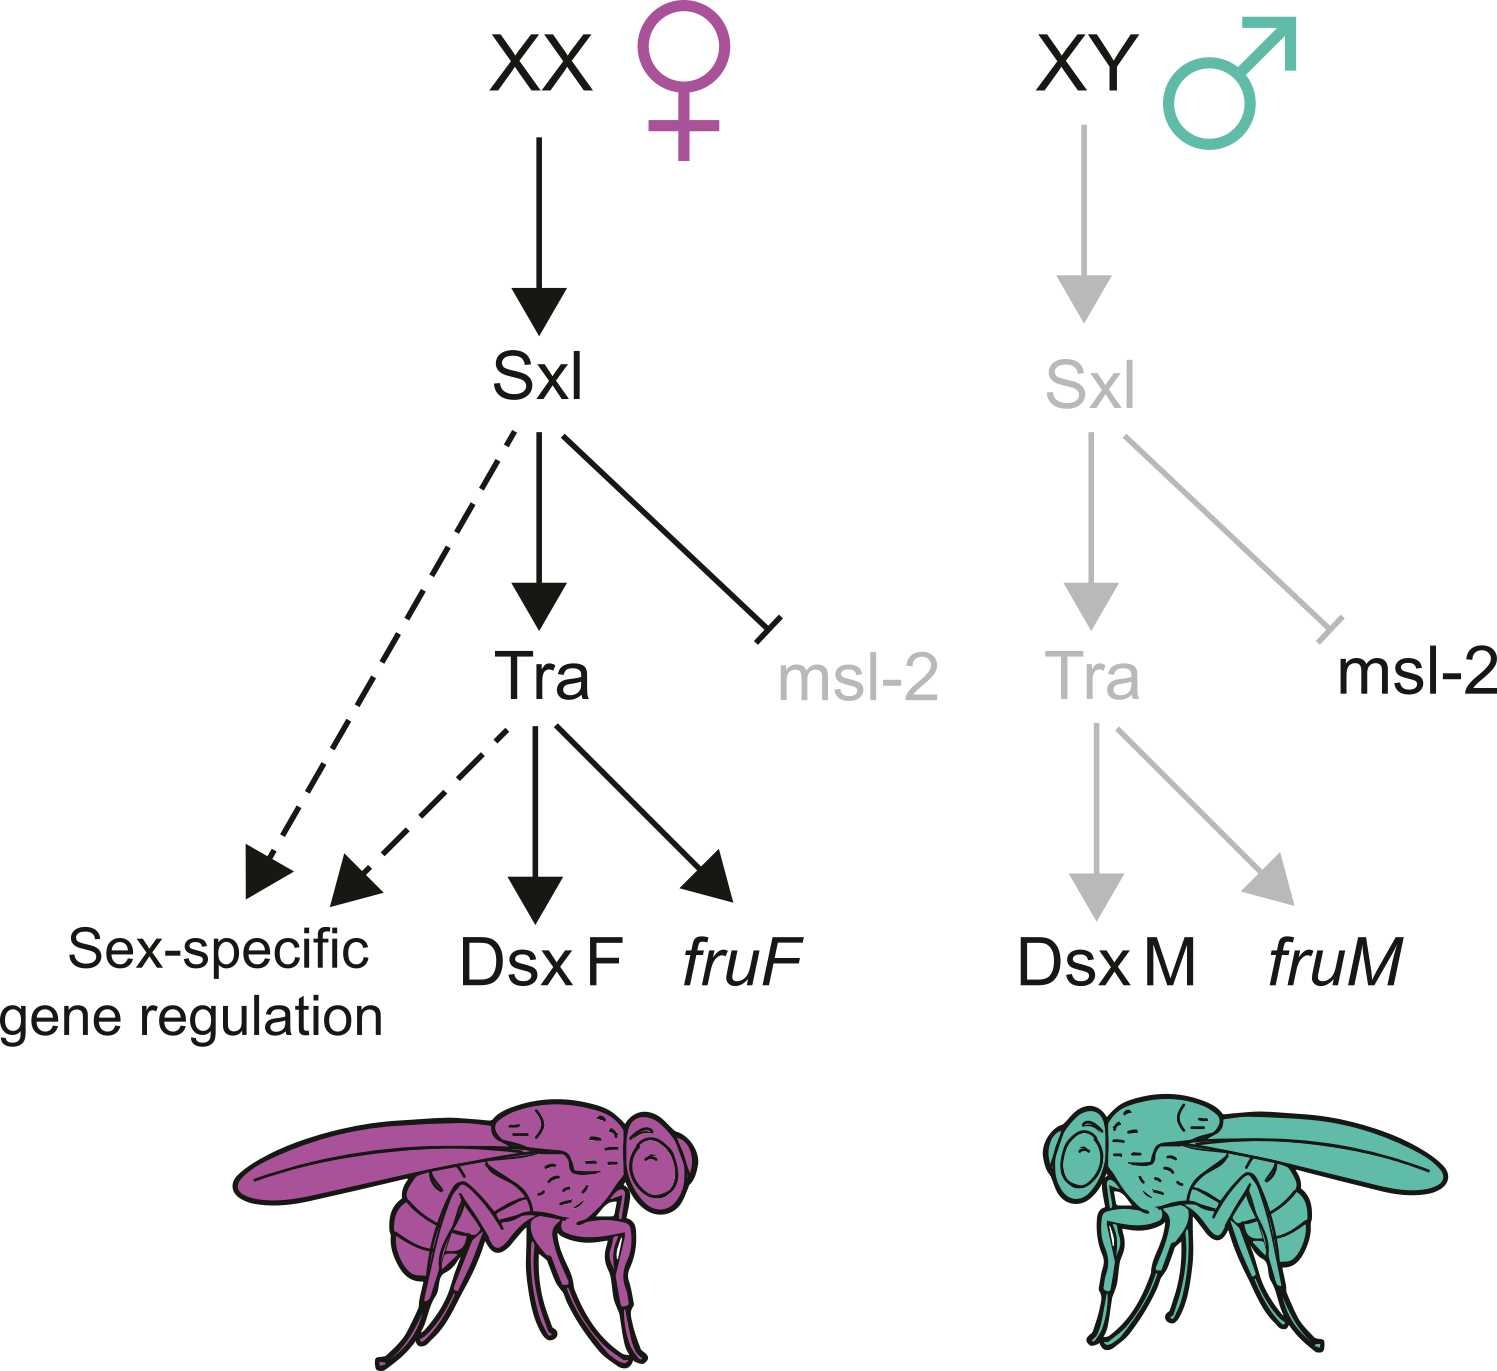
\includegraphics[alt = "A pair of diagrams showing how the Drosophila sex specific signaling pathways differ.", width=0.7\textwidth]{sexspecifichormones.jpg}
    \caption{from Shingleton and Vea (2023). Functional parts of the cascade are shown in black, non-functional parts are shown in gray. The possession of two X chromosomes leads to the synthesis of Sxl, which splices \textit{tra} pre-mRNA to generate a functional protein in females only. Functional Tra in turn splices \textit{dsx} pre-mRNA to generate the female isoform of Dsx (DsxF). In males, in the absence of Sxl and functional Tra, \textit{dsx} pre-mRNA is spliced to generate the male isoform of Dsx (DsxM). Functional Tra also directs the splicing of \textit{fru} pre-mRNA into a female isoform (\textit{fruF}) that is not translated, while the absence of functional Tra in males results in the default splicing of \textit{fru} pre-mRNA into a male isoform (\textit{fruM}) that is translated into functional protein. Active Sxl also suppresses the synthesis of the dosage compensation protein msl-2 in females, which otherwise heightens the activity of the single X chromosomes in males.}
    \label{fig:shingletongvea2023}
\end{figure}

Sex in \textit{Drosophila} is genetically determined via an XY system, and relies on the X-to-autosome ratio (\textbf{Figure 1}) (Pennell \& Morrow, 2013; Shingleton \& Vea, 2023). The possession of two X chromosomes leads to the synthesis of the \textit{Sex-lethal} protein (\textit{Sxl}) in females  (Salz, 2011; Shingleton \& Vea, 2023). \textit{Sxl} in turn initiates an expression cascade that affects all aspects of sexual dimorphism in \textit{Drosophila} (Salz, 2011). \textit{Sxl} does this by directing the synthesis of functional \textit{Transformer} (\textit{Tra}) in females, through alternative splicing, which in turn directs the alternative splicing of \textit{doublesex} (\textit{dsx}) and \textit{fruitless} (\textit{Fru}) into their female isoforms (Salz, 2011). The female isoform of \textit{doublesex} is translated into a protein that controls the female expression of phenotype (Deshmukh et al., 2020), while the female isoform of \textit{Fru} is not translated into functional protein (Rideout et al., 2007). In males, the absence of functional \textit{Tra} results in the default splicing of \textit{dsx} and \textit{Fru} into male-specific isoforms (Rideout et al., 2007). Both are translated into protein and direct the development of male morphology and male behavior, respectively (Rideout et al., 2007; Shingleton \& Vea, 2023).

Male and female \textit{Drosophila} are therefore more-or-less genetically identical -- what differs between the sexes is not so much the genes they carry, but the genes they express. This is generally true for all sexually dimorphic species, regardless of the genetic basis of sex determination (Fairbairn \& Roff, 2006; Wyman et al., 2013). This has profound implications for the evolution of SSD: Because males and females share a largely identical genome, and the same alleles are found in both male and female bodies, selection for different optimal traits, including body size, in each sex creates intralocus sexual conflict (IASC) (Lande, 1980; Bonduriansky \& Chenoweth, 2009) (as I will discuss further in Chapter 2).

\section{Sex-Specific Selection}

Sexual dimorphism, the morphological differences between females and males at the same developmental stage within a species, has been studied for over two centuries. Darwin was among the first to suggest that dimorphism evolves in response to male-male conflict and female mating choice (1871). Since then, it has become clear that sex-specific phenotypic optima also evolve in response to pressures around courtship, mating, fecundity, parental roles, and the environment (Anderson \& Iwasa, 1994; Lande, 1980).

Anisogamy, or the difference in morphology or size of female and male gametes, is both a cause and a consequence of sex-specific selection (Fairbairn, 1997). Males produce sperm, which are small and energetically inexpensive to generate in large quantities (Andersson \& Iwasa, 1994; Bateman, 1948; Bjork \& Pitnick, 2006). Consequently, a male's reproductive success is generally limited by his access to eggs and females (Andersson \& Iwasa, 1994; Bateman, 1948). Ova, however, are typically larger and more energetically expensive, thus females invest more to ensure offspring survival (Andersson \& Iwasa, 1994; Bateman, 1948). Thus, female reproductive success is limited by fecundity, or the number of eggs females can produce. Consequently, there is selection on males to increase their access to females, either through male-male competition or by increasing their 'attractiveness' to females (called intrasexual and intersexual selection respectively) (Andersson \& Iwasa, 1994; Bateman, 1948). In contrast, there will be selection on females to increase the number of eggs that an individual can produce (called fecundity selection), and to increase the quality of the sperm used to fertilize those eggs, and by extension the quality of offspring these sperm help generate, by being selective about which male(s) sire their offspring (intrasexual selection) (Andersson \& Iwasa, 1994; Bateman, 1948). The difference in gamete cost is therefore what ultimately drives the evolution of sex-specific behaviors and phenotypes (Bjork \& Pitnick, 2006).

Male-male intrasexual competition is common among sexually reproducing species, with males trying to secure as many matings as possible. This is perhaps most obvious in species that participate in lek mating, in which males provide females only with gametes (Gibson \& Bradbury, 1985; Rathore et al., 2023). Among lekking species, members of both sexes will gather, males will compete directly with one another through combat or elaborate displays for access to females (Gibson \& Bradbury, 1985; Rathore et al., 2023).

Copulation does not guarantee reproductive success, however. Among species that have females that mate with multiple males, females may evolve mechanisms to select which sperm they use to fertilize their eggs (Bjork \& Pitnick, 2006; Droge-Young et al., 2016; McDonough-Goldstein et al., 2022; Wagner et al., 2004). If a female's success is predicated on the quality of her offspring, her ability to choose the sire(s) is invaluable. Hence, in many species, female choice can take place after copulating with multiple males. For example, shortly after mating females can eject the sperm of undesirable males, as seen among birds like the black-legged kittiwake \textit{Rissa tridactyla} (Wagner et al., 2004) and the dunnock \textit{Prunella modularis} (Davies, 1983) and among insects such as the flour beetle \textit{Tribolium castaneum} (Droge-Young et al., 2016) and \textit{D. melanogaster} (McDonough-Goldstein et al., 2022). Sperm can also be subject to cryptic female choice. Cryptic female choice typically refers to sperm selection that occurs within the female body, though it cannot be easily observed (Birkhead, 1998; Bjork \& Pitnick, 2006). For example, in \textit{Drosophila} females select for the longest sperm (Lüpold et al., 2016; Pitnick et al., 1995). 

In response to these female strategies, males have evolved their own post-copulatory tools and strategies to interfere with female choice and reduce sperm competition. To minimize sperm competition, the males of some species will guard females during the mating period, preventing other males from copulating (Andersson \& Iwasa, 1994). Mate guarding is seen in both vertebrates, particularly birds (Sherman, 1989), and invertebrates (Simmons, 1990; Jormalainen, 1998). Another way males can minimize sperm competition is by using mating plugs, which block the female reproductive tract and reduce the chances of subsequent matings resulting in fertilization. Mating plugs are common in invertebrates including \textit{Drosophila melanogaster} (Lung \& Wolfner, 2001), but are also made by some vertebrates such as \textit{Lacerta monticola}, a species of lizard (Moreira \& Birkhead, 2003). Males may also leave the females covered in anti-aphrodisiacs, or pheromones that make females seem unattractive, thus deterring other males from copulating with them. Anti-aphrodisiacs are common among butterflies (Estrada et al., 2011), but are also used by \textit{Drosophila melanogaster} (Laturney \& Billeter, 2016). Some male reproductive anatomy has evolved to serve not only as a means of insemination but also as a tool to reduce sperm competition. For example, the males of \textit{Calopteryx maculata}, a species of damselfly, have structures used during copulation to remove sperm from a female's previous matings (Waage, 1979). Intense sperm competition and cryptic female choice can also result in evolutionary pressures on sperm morphology and size. For example, \textit{Drosophila bifurca} have sperm 5.8 cm long, or about 20 times their body length (Lüpold et al., 2016; Pitnick et al., 1995). 

Collectively, these persistent sex-specific selective pressures drive the evolution of increasingly complex behavioral and morphological differences between sexes. However, because males and females share a largely identical genome (Fairbairn \& Roff, 2006; Wyman et al., 2013), these sex specific optima introduce potential genetic conflict for traits shared by both sexes, a phenomenon known as sexual conflict (Lande, 1980; Bonduriansky \& Chenoweth, 2009). When the same genes influence a trait with different fitness optima in males and females, selection applied to one sex can generate a corresponding response in the other sex, which may be selected against (Fisher, 1958; Bird \& Schaffer, 1972; Lande, 1980; Bonduriansky \& Chenoweth, 2009; Sayadi et al., 2019). The resulting tug of war, with alleles being selected \textit{for} in one sex, and \textit{against} in the other, can constrain each sex from reaching its phenotypic optimum (Fisher, 1958; Bird \& Schaffer, 1972; Lande, 1980). Therefore, sexual conflict may play a key role in shaping how sexual dimorphism responds to artificial selection (as I will discuss further in Chapter 2).

Thus, while we understand the selective pressures that generate sexual dimorphism and the sex determination cascades that result in sex-specific gene expression, we do not understand the specific developmental-genetic mechanisms that generate sexual dimorphism.

\section{Sexual Size Dimorphism}

Perhaps the most obvious form of sexual dimorphism is sexual size dimorphism (SSD). Female-biased SSD (i.e., females larger than males) is common among fish, birds, reptiles, and arthropods, including \textit{D. melanogaster} (Fairbairn, 1997; Testa et al., 2013; Webb \& Freckleton, 2007), while male-biased SSD is common among mammals (Fairbairn, 1997; Isaac, 2005). 

Despite decades of research, there is no consensus explaining the evolutionary mechanisms that generate SSD though several patterns have emerged. Rensch's rule states that among species with female-biased SSD, the degree of SSD typically decreases with increasing species body size, while among species with male-biased SSD, it typically increases with increasing species body size. A link has also been suggested between the evolution of sex-determination mechanisms and SSD, with the heterogametic sex usually being the larger sex in both XY and ZW systems (Adkins-Regan \& Reeve, 2014; Schwanz et al., 2016). 

However, there is no consensus explaining the evolutionary mechanisms that generate SSD. One approach to better understand the ultimate mechanisms underlying SSD might be to focus on the proximate, developmental-genetic mechanisms regulating SSD. Though sex determination and the selective pressures that result in observed patterns of SSD have been well studied, how SSD occurs at the developmental-genetic level remains largely unknown. Understanding the developmental-genetic mechanisms underlying SSD will provide insight into the evolution and development of SSD.

\begin{figure}[htbp]
    \centering
    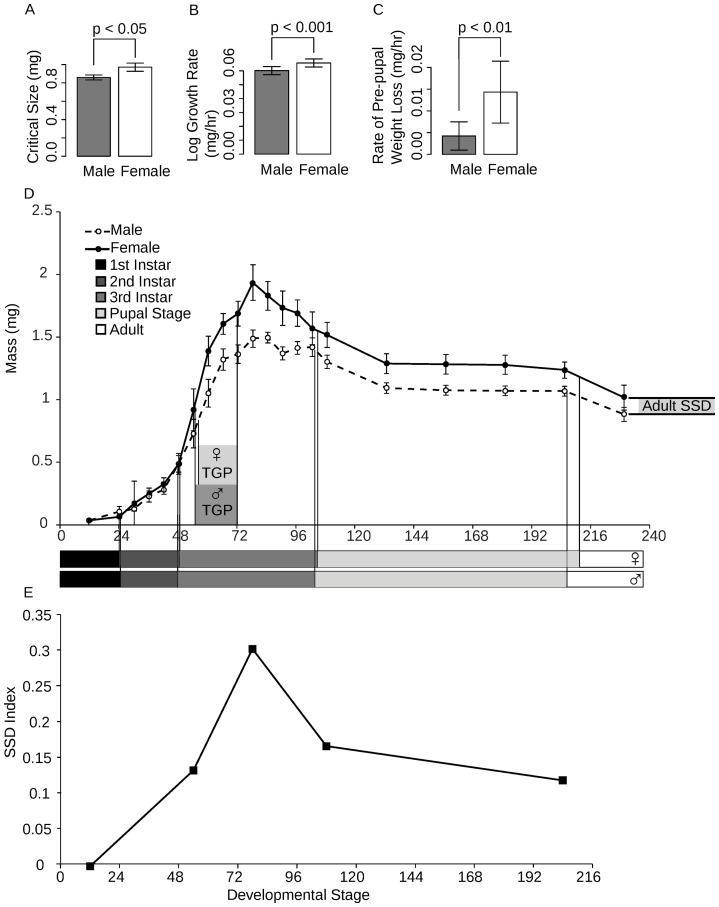
\includegraphics[alt = "Sex specific growth curves of D. melanogaster showing how adult sexual size dimorphism is the accumulation of sex specific differences in growth during development.", width=0.8\textwidth]{testafig1.jpg}
    \caption{from Testa et al., 2013. Complete growth profile by sex for Drosophila melanogaster. Factors shown to contribute to SSD include (a) critical size, (b) growth rate, (c) and pre-pupal weight loss and are reflected in the sex-specific growth curve (d). The SSD at specific developmental events (hatching, critical size, peak larval mass, pupariation and eclosion) illustrates the changes in SSD throughout development (e). Error bars show 95\% confidence intervals.}
    \label{fig:testa2013a}
\end{figure}

\section{Developmental Mechanisms Regulating body size}

Generally, adult body size in animals is regulated by four developmental factors: (1) size at birth/hatching, (2) growth rate, (3) growth duration, and (4) mass loss during development (Testa et al., 2013). Changes in any of these factors alter adult body size, consequently sex-specific differences in these factors generate SSD (Testa et al., 2013). Nevertheless, the molecular, genetic, and physiological regulators of these developmental factors are poorly understood, with the exception of a few model organisms. 

Of all animals, these regulators are best understood in \textit{D. melanogaster}, which has long been used in developmental genetics research (Shingleton \& Vea, 2023). \textit{Drosophila} is a holometabolous insect that molts through three larval instars before pupating and metamorphosing into the final adult form. Before pupariation, third-instar larvae must reach critical size, the size at which they initiate the hormonal cascade that causes the synthesis of ecdysone, which drives metamorphosis and the cessation of growth (Nijhout et al., 2014). The release of ecdysone initially triggers larval wandering, which is when feeding stops and the larvae search for a pupariation site (Nijhout et al., 2014; Testa et al., 2013). Growth of overall body size is restricted to the larval period, so adult body size is essentially fixed by larval body size at pupariation (Testa et al., 2013). Thus, the factors regulating adult body size are (1) critical size, (2) the time between attaining critical size and larval wandering, called the terminal growth period (TGP), (3) the rate of growth during TGP, and (4) mass loss during wandering (Ghosh et al., 2013; Shingleton \& Vea, 2023). Of these, sex-specific differences in critical size, growth rate during TGP, and mass loss appear to regulate SSD (Testa et al., 2013; Shingleton \& Vea, 2023). 

We have an increasingly good understanding of the developmental genetic mechanisms that regulate critical size, growth rate, and mass loss. In particular, work in \textit{Drosophila} over the past three decades has illuminated the critical role the insulin/insulin-like growth factor signaling (IIS) and Target of Rapamycin (TOR) pathways play in the regulation of growth and body size (Rideout et al., 2015; Testa et al., 2013; Texada et al., 2020;  Mirth \& Shingleton, 2012). The IIS and TOR pathways are highly conserved regulators of growth in metazoans, adjusting in response to the environment, specifically the nutritional environment with the IIS pathway adjusting at a systemic level and the TOR pathway adjusting at a cellular level (Grewal, 2008; Texada et al, 2020). When nutrients are abundant, the level of circulating insulin is high and the IIS and TOR pathways promote growth. In contrast, when nutrition is low, insulin levels drop, suppressing IIS/TOR activity and growth. IIS/TOR therefore functions to regulate body size specifically in response to the nutritional environment. 

\begin{figure}[b!]
    \centering
    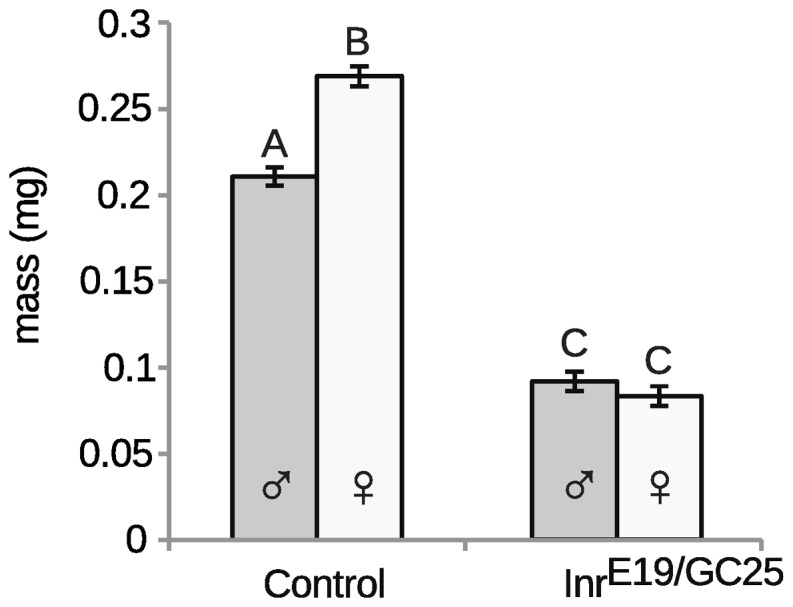
\includegraphics[alt = "A plot showing how if insulin signalling is knocked down there is no sexual size dimorphism.", width=0.6\textwidth]{testafig2.jpg}
    \caption{from Testa et al., 2013. SSD is lost in insulin-signaling mutants. The dry mass of male and female adult $Inr^{E19}$/$Inr^{GC25}$ and wild-type ($Inr^{E19}$/$TM3$) control flies reared at low density at 24\si{\celsius}C. Columns with different letters are significantly different (Tukey HSD at $p$<0.05). Error bars are standard errors.}
    \label{fig:testa2013b}
\end{figure}
        
\section{Insulin is Necessary for SSD}

While we know the developmental-genetic mechanisms underlying body size, how these mechanisms operate to generate SSD remains unclear. A recent discovery, however, is that knockdown of IIS eliminates SSD in \textit{Drosophila} (\textbf{Figure 3}) (Testa et al., 2013). That is, a functional IIS pathway is necessary to generate SSD. Subsequent research suggests that females have higher levels of IIS activity than males (Rideout et al., 2015). It follows that, if IIS is necessary for SSD and females have higher IIS activity, then female body size should be more sensitive to changes in IIS, and nutrition in  than male body size. IIS is regulated by nutrition, so it also follows that body size in females should be more sensitive to changes in developmental nutrition than males. That is, female body size should be more nutritionally plastic than male body size, where plasticity refers to the effect of the environment on phenotype independent of genotype (Lande, 2014). This is called sex-specific plasticity (SSP). Since SSP inherently generates SSD, at least in some environmental conditions, observed SSD may therefore be a consequence of selection for SSP (Shingleton \& Vea, 2023; Vea et al., 2023). Thus, the sex-specific regulation of IIS in response to nutrition is likely a key developmental genetic mechanism underlying SSD.

\section{Sex-Specific Plasticity (SSP) and SSD}

The observation that SSD is regulated by IIS in \textit{D. melanogaster} and that females are more insulin-sensitive than males, suggests that body size in females should also be more nutritionally plastic than males, a phenomenon called sex-specific plasticity (SSP). This is indeed the case. Previous work from Vea et al. (2023) used 186 lineages from the \textit{Drosophila} Genetic Reference Panel (DGRP) (Mackay et al., 2012) demonstrated that genetic variation in SSD is correlated with sex-specific plasticity (SSP), suggesting SSP and SSD are regulated by the same developmental-genetic mechanisms. Though the work of Vea et al. (2023) suggests overlap in the mechanisms responsible for SSP and SSD, the loci underlying the variation they observed have yet to be identified. Identifying the loci responsible for SSD and SSP in \textit{Drosophila} will provide insight into how SSD and SSP (co)evolve on the developmental-genetic level. If selection is actually acting on SSP to generate SSD, the developmental mechanisms that underlie variation in SSD overlap with those that underlie SSP. 

\section{Vea et al.'s (2026) GWAS on SSP and SSD}

To identify the genes underlying variation in SSD and SSP, Vea et al (2026) conducted Genome Wide Association Study (GWAS) on DGRP lineages. While GWASs can identify standing variation in existing populations, GWASs do not indicate which subset of candidate loci is actually targeted by selection--a particular challenge for quantitative traits that are likely polygenic and therefore have a large target for selection, such as SSD (Turner et al., 2013). An Evolve and Resequence (E\&R) study, however, does provide insight into the evolution of such traits by applying artificial selection and observing which loci were targeted (Kofler \& Schlötterer, 2013; Turner et al., 2013).

\section{GWAS and E\&R as Complementary Approaches}

GWAS and E\&R have previously been used in tandem to identify the genes associated with \textit{Drosophila} courtship song (Turner et al., 2013). Although Turner et al. (2013) found no highly significant single-nucleotide polymorphisms (SNPs) in either GWAS or E\&R individually, they identified 101 SNPs with high differentiation in the E\&R study and low \(p\)-values in the GWAS, which were associated with 42 genes. Thus, by leveraging both approaches, Turner et al. (2013) identified candidate genes likely responsible for variation in courtship song.

Using GWAS and E\&R in tandem is therefore a powerful approach to elucidate the genes that regulate SSD and the evolution and development of SSD. Vea et al. (2026) conducted a GWAS for SSD and SSP and identified 110 candidate genes. As a complementary approach, I used E\&R by first artificially selecting for SSD (and thus possibly indirectly for SSP) and then identifying the loci that have been targeted (discussed further in Chapters 2 and 3). Genes identified by the DGRP GWAS and my E\&R study are likely the alleles involved in the regulation of SSD. %SOMETHING ABOUT MAYBE HITTING THE SAME LOCI IDENTIFIED BY GWAS FOR SSP MAYBE

\section{SSD can be Changed by Artificial Selection}

The intensity and direction of SSD can differ between species in the same family or even genus (Cox et al., 2003; Fairbairn, 1997; Slavenco et al., 2025). This suggests that SSD has considerable intraspecific variation and can therefore be changed by artificial selection. Tigreros and Lewis (2011) briefly selected on SSD of the red flour beetle \(Tribolium\) \(castaneum\) using pupal mass as the metric for body size. There were three selection regimes, (1) concordant for increasing size, (2) concordant for decreasing size, and (3) discordant selection. However, for the discordant lineage, they were not successful at evolving SSD after applying selection for only seven generations; both sexes experienced a similar increase or decrease in mass with each generation in all lines.

In contrast, Stewart and Rice (2018) applied discordant selection on body size in \textit{D. melanogaster} for 250 generations and successfully reversed the direction of SSD from female-biased to male-biased after approximately 175 generations of sex-discordant selection. A subsequent genomic analysis of these discordant lineages identified 295 candidate genes, 11 of which have both a sex-limited phenotype and a known size phenotype (Audet et al., 2024). However, none of these candidate genes have been functionally tested to confirm their involvement in the regulation of SSD.

In another experiment, Bird and Schaffer (1972) artificially selected on the magnitude of sexual dimorphism of the wings of \textit{D. melanogaster} over fifty years ago. Because sexual dimorphism is a group trait and, therefore, cannot be selected at the individual level, they compared average sex specific wing sizes between full siblings. Sibling sets with the largest sex difference were crossed to produce a high dimorphism lineage, while those with the smallest sex difference were crossed to produce a low dimorphism lineage. After only 15 generations, they generated divergent lineages that maintained their dimorphism after ten generations of relaxed selection, demonstrating that they had successfully targeted the developmental-genetic mechanisms underlying sex-specific wing size. 

Bird and Schaffer's (1972) selection experiment was conducted at a time when our understanding of developmental mechanisms and genetics was limited, making it impossible to identify the mechanisms responsible for the difference they observed. My E\&R study uses family selection on SSD and does what Bird \& Schaffer could not do by making use of modern genetic resources. Some of these resources--such as PoolSeq (Anand et al., 2016) and E\&R adapted chi-square tests (Spitzer et al., 2019)--have been specifically designed for E\&R studies.

\section{Rationale for an E\&R Study on SSD}

Sexual size dimorphism (SSD) in \textit{Drosophila} is a result of sex-specific differences in critical size, growth rate during the terminal growth period (TGP), and mass loss (Testa et al., 2013). \textit{Drosophila}'s Insulin/IGF Signaling (IIS) pathway regulates growth in response to nutrition and is necessary to generate SSD (Testa et al., 2013). Furthermore, female body size is more nutritionally plastic than male body size, and this sex-specific plasticity (SSP) is tightly genetically correlated with SSD, suggesting the two phenomena share developmental-genetic mechanisms (Rideout et al., 2015; Vea et al., 2023). Despite this progress, the developmental-genetic mechanisms regulating SSD remain largely unknown. 

Resolving this gap is important for several reasons. First, identifying these mechanisms can shed light on how sex-specific selection acts on a shared genome and resolves intralocus sexual conflict (IASC) (Bonduriansky \& Chenoweth, 2009; Kasimatis et al., 2017). Second, because SSD is tightly correlated to SSP (Vea et al., 2023), identifying these mechanisms may reveal how factors like nutrition differentially affect male and female growth. Third, most research on growth regulation has focused on males, yet females and males exhibit fundamentally different cellular and molecular mechanisms even when producing similar phenotypic outcomes (Mank \& Rideout, 2018). These differences mean that findings from male-biased studies cannot be simply generalized to females (Clayton, 2015; Mank \& Rideout, 2018). Research focused on only one sex in light of sexual dimorphism not only limits our understanding of basic biological processes, but has important implication for human health (Clayton, 2015; Mank \& Rideout). For this reason, NIH recently imposed a requirement that physiological studies include members of both sexes (NIH, 2015). Thus, a comprehensive understanding of growth regulation requires studying both sexes together. By identifying the genetic mechanisms underlying SSD--a trait defined by the differences in growth between sexes--my research directly addresses this gap.

To complement Vea et al.'s (2026) GWAS on SSD, I have conducted an Evolve and Resequence (E\&R) experiment. E\&R uses artificial selection to drive phenotypic change to increase the frequency of causative alleles (Kofler \& Schlötterer, 2013; Turner et al., 2013). By comparing initial and final populations, we can identify loci associated with the desired phenotype (Kofler \& Schlötterer, 2013). This method has already been used in tandem with a GWAS to identify the loci responsible for \textit{Drosophila} courtship song (Turner et al., 2013).

In the following chapters I will detail my work towards understanding the mechanisms underlying SSD: 

\begin{itemize}
\item \textbf{Chapter 2:} I describe the \textit{Evolve} portion of my E\&R study, presenting how 15 generations of family selection generated divergent SSD lineages and revealing asymmetric responses between the sexes that point to sexual conflict.
\item \textbf{Chapter 3:} I describe the \textit{Resequence} portion of my E\&R study, comparing allele frequencies between ancestral and selected populations and intersecting these results with Vea et al.'s (2026) GWAS to identify high-confidence candidate genes.
\item \textbf{Chapter 4:} Using isogenized lineages derived from the final selected populations, I ask whether a single developmental trait—such as minimum viable weight, developmental timing, or growth rate—can explain the divergence in SSD, or whether SSD instead emerges from a suite of interconnected changes. I also characterize consequential traits (fecundity, viability, lifespan) to explore the fitness consequences of altering SSD beyond that found in nature.
\item \textbf{Chapter 5:} I synthesize the findings from the preceding chapters, discuss the implications for understanding the evolution and development of SSD, and propose future directions.
\end{itemize}

Please note that each chapter is written as a stand-alone paper, there will be some repetitive content.

\newpage
\chapter{Artificial Selection on Sexual Size Dimorphism} 

The difference between male and female body size (sexual size dimorphism, SSD), is one of the most obvious ways in which the sexes differ. Research over the last three decades established the developmental, genetic, and physiological mechanisms that regulate body size in \textit{Drosophila melanogaster}, a species that exhibits SSD with females as the larger sex (Mirth \& Shingleton, 2015; Reeve \& Fairbairn, 1999; Testa et al., 2013; Webb \& Freckleton, 2007). It is well understood that females and males are essentially genetically identical (Fairbairn \& Roff, 2006; Kasimatis et al., 2017; Reeve \& Fairbairn, 1999; Wyman et al., 2013) and that sex determination is the result of differences in gene expression, which ultimately generate SSD (Mank, 2017; Price et al., 2023; Shingleton \& Vea, 2023). However, while sex determination and the selective pressures that produce observed patterns of SSD have been well studied (Fairbairn, 1997; Lande, 1980; Mank, 2017; Price et al., 2023; Shingleton \& Vea, 2023), how SSD occurs at the developmental-genetic level remains largely unknown. Identifying the genes and pathways that regulate SSD is therefore a critical step toward understanding how SSD evolves.

Generally, adult body size in animals is regulated by four developmental factors: (1) size at birth/hatching, (2) growth rate, (3) growth duration, and (4) mass loss (Testa et al., 2013). Sex-specific differences in any of these factors can generate SSD. The molecular, genetic, and physiological regulators  of these factors are best understood in \textit{D. melanogaster} (Shingleton \& Vea, 2023). \textit{D. melanogaster} is a holometabolous insect that molts through three larval instars before pupating and metamorphosing into the final adult form. Third-instar larvae must reach critical size to initiate the hormonal cascade that triggers metamorphosis and stops growth (Nijhout et al., 2014; Testa et al., 2013). After reaching critical size, larvae enter the terminal growth period (TGP) before wandering, which is when feeding stops and the larvae search for a pupariation site (Nijhout et al., 2014; Testa et al., 2013). Thus, we can think of the four factors regulating adult body size in \textit{Drosophila} as (1) critical size, (2) TGP duration, (3) growth rate during TGP, and (4) mass loss during wandering (Ghosh et al., 2013; Shingleton \& Vea, 2023). Of these, sex-specific differences in critical size, growth rate during TGP, and mass loss accumulate to generate adult SSD (Testa et al., 2013; Shingleton \& Vea, 2023). Yet, how these traits respond to selection on SSD has never been directly tested.

\section{Identifying Mechanisms That Underlie SSD}

A widely used approach to identify the genetic basis of a quantitative phenotype is a genome wide association study (GWAS) (Visscher et al., 2012), which compares variation in phenotype and genotype across existing populations to identify candidate genes associated with the trait of interest (Tam et al., 2019; Visscher et al., 2012). A complementary approach to identify the genetic basis of a quantitative phenotype is the Evolve and Resequence (E\&R) study, which uses artificial selection to drive phenotypic change, thereby increasing the frequency of causative alleles (Kofler \& Schlötterer, 2013; Turner et al., 2013). Loci that respond to selection are identified by comparing genomes of selected and unselected populations (Kofler \& Schlötterer, 2013; Vlachos \& Kofler, 2019). E\&R not only identifies the genes associated with trait of interest but also provides insight into how the trait of interest evolves in response to selection. In combination, therefore, GWAS identifies the loci that underlie standing genetic variation for a trait, while E\&R identifies which of these loci are targeted by selection to generate the phenotypic change of interest. GWAS and E\&R are complementary approaches and have been used in combination to successfully identify the genes underlying \textit{D. melanogaster} courtship song (Turner et al., 2013).

Here I use E\&R as a complementary approach to a previous GWAS to (1) identify the developmental-genetic mechanisms that regulate SSD in \textit{D. melanogaster} and (2) explore which aspects of these mechanisms can be targeted by selection to generate evolved changes in SSD. The previous GWAS not only established that there is ample standing genetic variation in SSD in \textit{D. melanogaster}, but identified 110 loci associated with this variation (Vea et al., 2026). Intriguingly, almost none of those loci lay within genes currently characterized as regulators of SSD, specifically genes involved in the nutritional regulation of body size (Testa, 2013; Vea et al. 2026). Body size is, however, a very large genetic target and is impacted by myriad genes. The results of the GWAS are perhaps, therefore, not unexpected. What is unclear is whether selection on SSD targets the subset of these loci specifically involved in the nutritional regulation of body size, as implied by other developmental studies on SSD (Rideout et al., 2015; Testa et al., 2013). 

Two artificial selection methods have been used to alter dimorphism. A recent study used discordant selection on male and female body size at a population level over 250 generations which reversed the direction of SSD around generation 175 (Stewart \& Rice, 2018). An older study leveraged family based selection on wing sexual dimorphism to change sexual dimorphism in 15 generations (Bird \& Schaffer, 1972). I used the family based selection approach as the basis for my E\&R study. I describe the phenotypic outcome of this selection in this chapter, assessing standing variation of the source population, assessing the response to selection (both direct and indirect), and discuss what the observed responses mean about the evolution of SSD. The genetic outcome of selection are described in Chapter 3.

\section{SSD is Evolvable}

The intensity and direction of SSD can differ between species of the same family or even genus (Cox et al., 2003; Fairbairn, 1997; Slavenco et al., 2025). This suggests that SSD has considerable intraspecific variation and can therefore be changed by selection. Previous work has found there is extensive variation in SSD among the DGRP, with a coefficient of variation of 0.33 (Vea et al., 2023), suggesting \textit{D. melanogaster} population harbor ample variation on which selection can act upon. More pertinently, Bird and Schaffer (1972) successfully selected on sexual dimorphism of wing size using family selection, generating divergent lineages in only 15 generations. However, their work was conducted at a time when it was not feasible to identify the loci underlying their selected phenotypes. Moreover, they selected on wing size rather than body size. 

Given that SSD is evolutionarily labile and Bird \& Schaffer's (1972) observed rapid evolution of sexual dimorphism, to identify the genetic basis of SSD expression and evolution I am using an E\&R study. I designed a 15-generation family selection experiment, adapted from Bird and Schaffer (1972), to generate lineages of divergent SSD using body size as the metric for selection. I used the Fenn Valley Winery (FVW) stock as my initial population. To assess the standing genetic variation in SSD within this stock, I analyzed the SSD of 66 isogenized lineages derived from the FVW stock over 10 generations of full-sibling inbreeding without selective pressure. Because these lineages originated from the same base population as my selection experiment and were maintained without selection, their variation in SSD reflects the genetic variation present in the FVW stock prior to selection. I used this to estimate the potential range of SSD phenotypes achievable through selection.

\section{Methods}

\subsection{Initial Population and Rearing Conditions} 

The initial population came from the out-bred super-colony FVW stock maintained in the Frankino lab. The FVW stock is a colony established in 2008 from more than sixty females collected from the Fenn Valley Winery in Michigan. The stock has been maintained at varying temperatures and diets to prevent adaptation to specific lab conditions and maintain genetic diversity. Throughout this experiment flies were fed a high protein diet (as described in Mirth et al. [2019]), maintained under 24-hour lighting at 22\si{\celsius}C, unless otherwise stated.

\subsection{Characterizing SSD of Isogenized FVW Lineages}
Pupal area was measured as the metric for body size using uManager and a semi-automated FIJI journal (code available on GitHub at \url{https://github.com/LizAgolli/Evolve-SSD}). These flies were reared across a nutritional gradient. Because previous studies showed SSD is reduced with decreased nutrition (Shingleton \& Vea, 2023), I used only the largest individuals from each lineage-sex combination (90th percentile and above) to calculate SSD. This approach assumes that under optimal conditions, genetic differences in growth potential are most clearly expressed. Lineages were included in the analysis only if at least five females and five males were present after filtering. A Markov chain Monte Carlo generalized linear mixed model with the R package \textit{MCMCglmm} was used to calculate the coefficient of variation of SSD, the correlation of sex specific size to SSD, and intersexual genetic correlation (adapted from Vea et al., 2023).

\subsection{Establishing the Lineages - Generation 0} 
Adult FVW flies were allowed to oviposit in bottles for 48 hours. Pupae were sexed at stage P13/P14 and 150 single female-male pairs were transferred as pupae to individual food vials to establish single-pair families. Following eclosion, the adult pairs were allowed 2-5 days to mate and oviposit, after which the parents were collected and stored dry at -80\si{\celsius}. The offspring were then sexed as pupae (P13/14), and at least eight male and eight female pupae from each family were put into single-sex vials and allowed to eclose at 17\si{\celsius}C. This generated two vials for each family: one for females and one for males. I measured pupal area using uManager and the same semi-automated FIJI journal used for the isogenized FVW lineages. SSD for each family was calculated as

\[|\hat{B}_{female} - \hat{B}_{male}| \; (\mu m^2)\]

\noindent where $\hat{B}$ is mean log body size. I selected 20 families at random to establish the control lineage (CL). The remaining 100 families were ranked based on SSD. The 20 families with the highest SSD were used to establish the high SSD lineage (HL) and the 20 families with the lowest SSD were used to establish the low SSD lineage (LL). 

The result was 120 vials, comprising male and female vials from 60 families (20 HL families, 20 LL families, 20 CL families) each with eight individuals (eight males, eight females). These vials were used for the initial crosses. 

\begin{figure}[ht]
    \centering
    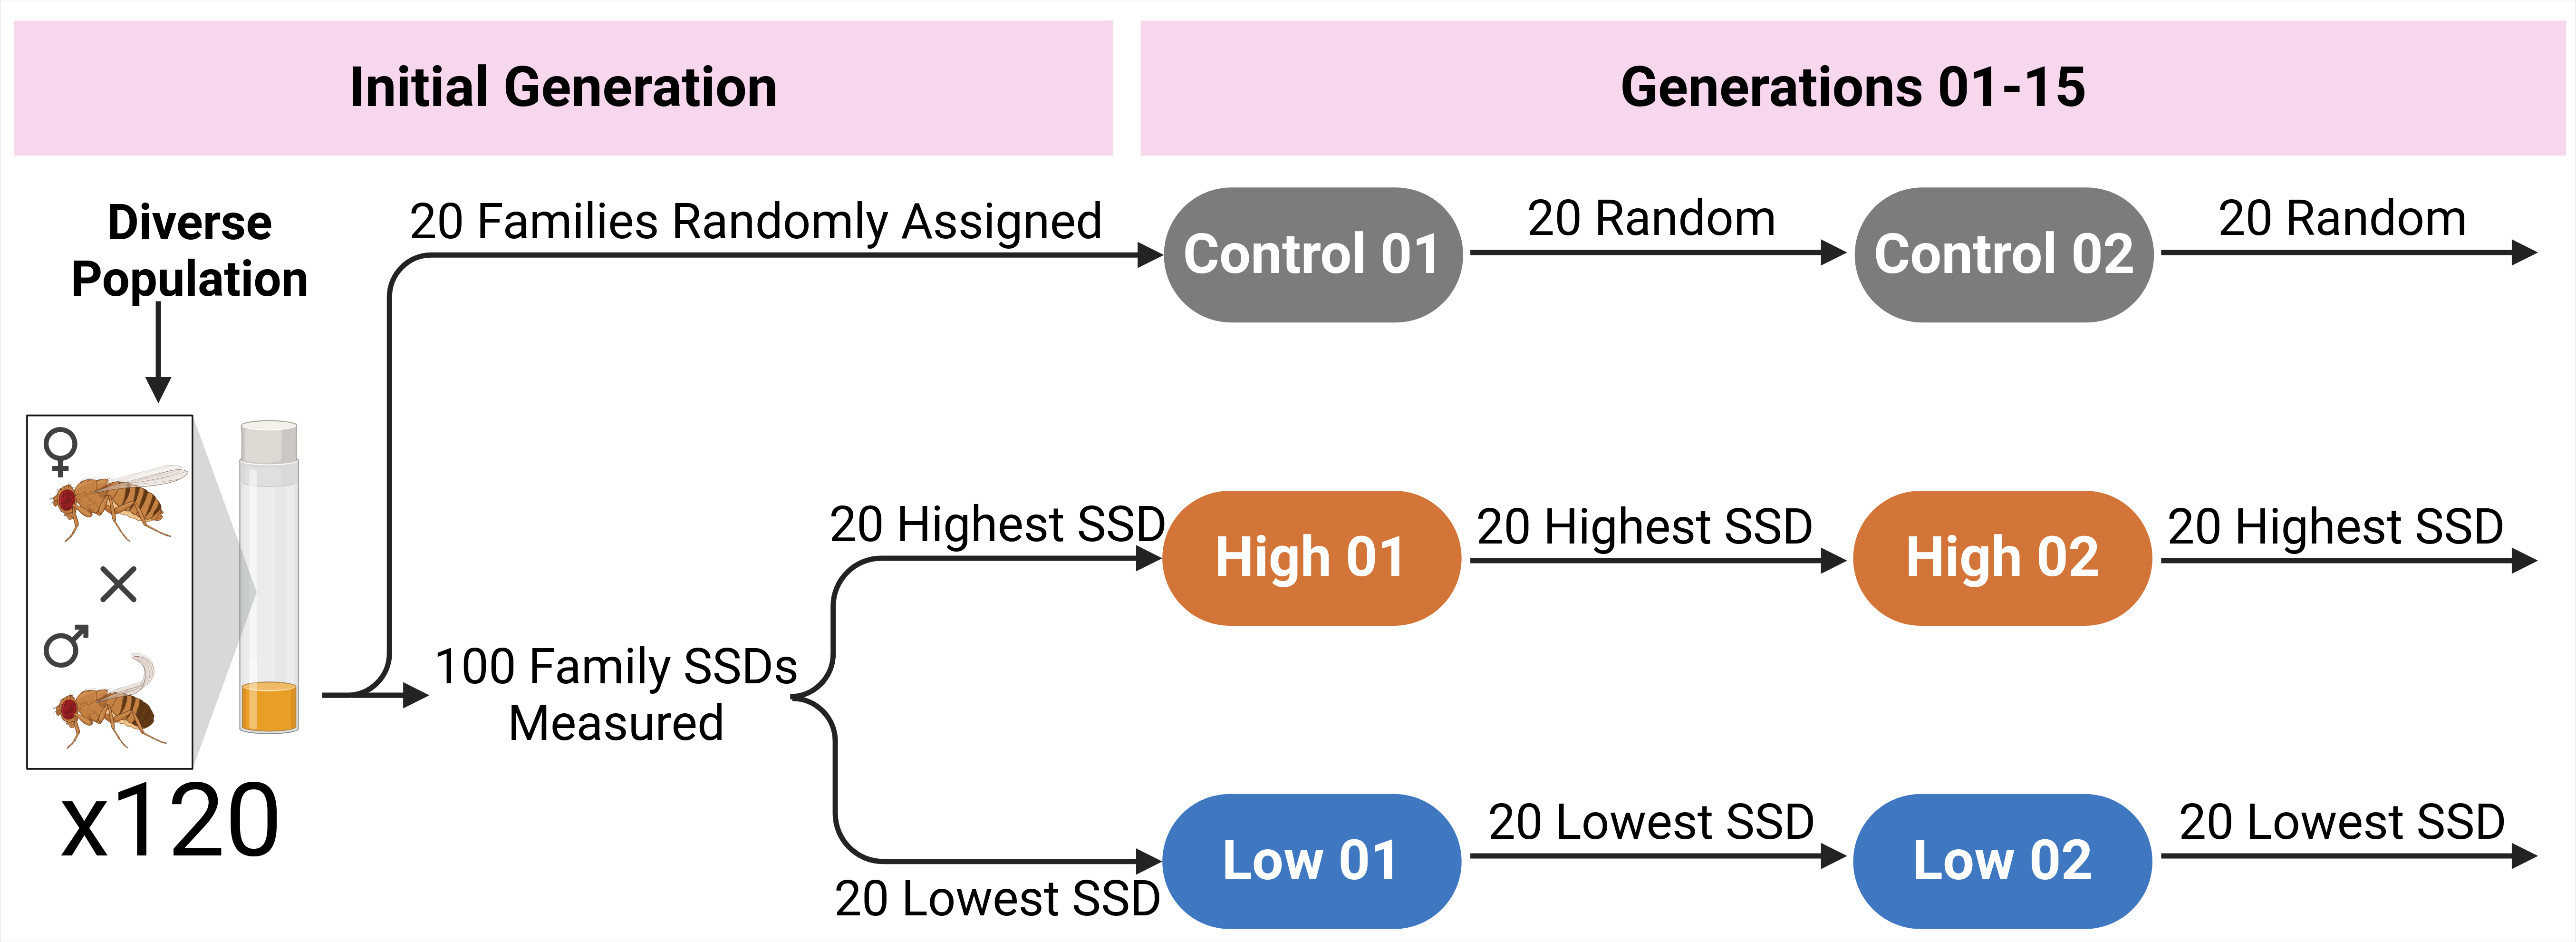
\includegraphics[alt = "Chart showing how lineages diverged from starting population.", width=1\textwidth]{Generation Selection Layout.jpeg}
    \caption{Overview of lineage divergence from the Fenn Valley Winery (FVW) colony. 120 single-pair crosses from the Fenn Valley Winery colony, with 20 randomly selected to found the Control Lineage (CL). Full sibling sets from the remaining 100 pairs had pupal area measured to determine SSD. The 20 with the highest SSD established the High SSD Lineage (HL) and the 20 with the lowest SSD established the Low SSD Lineage (LL). The selection criteria remained consistent for subsequent generations; 20 CL families selected at random, 20 HL families selected for having the highest SSD, and 20 LL families selected for having the lowest SSD.}
    \label{fig:genselection}
\end{figure}

\subsection{Selection Regime - Generations 1-15}
\textit{This selection regime was adapted from Bird and Schaffer (1972).}

\begin{figure}[b!]
    \centering
    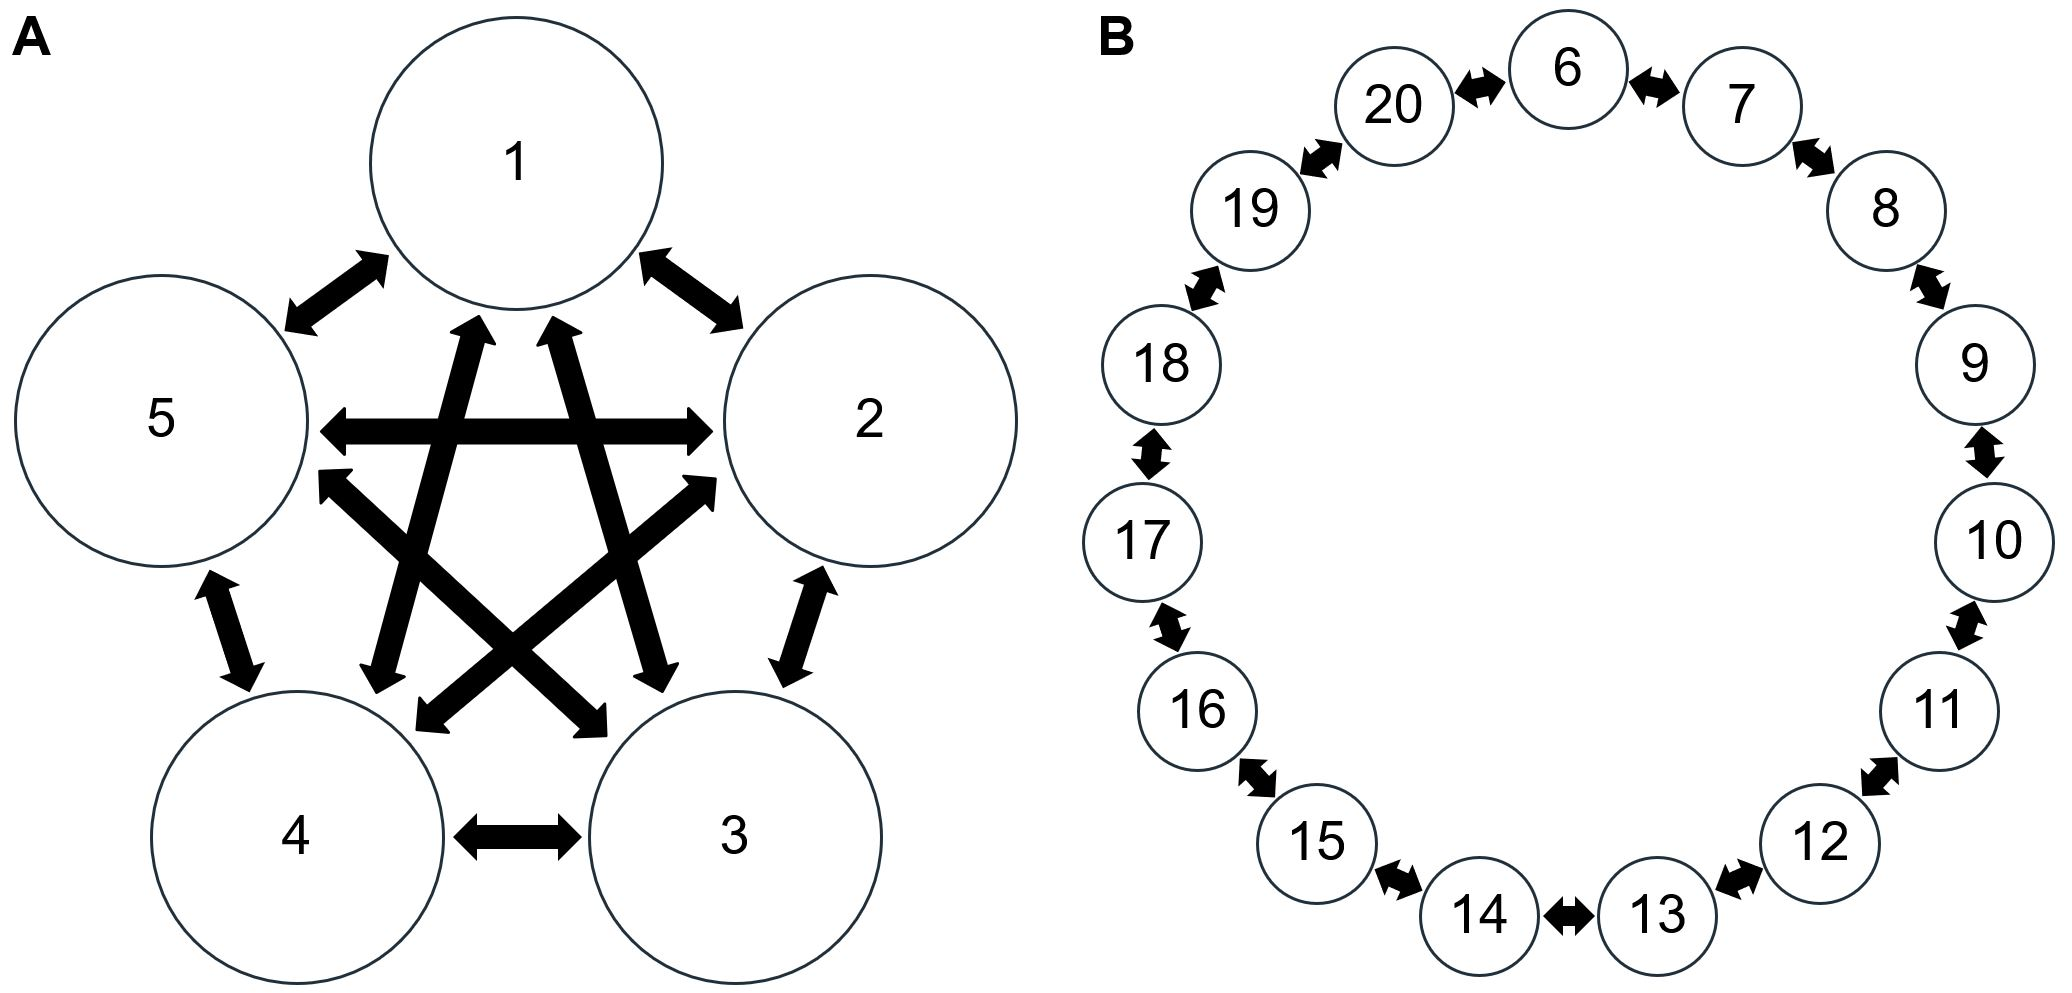
\includegraphics[alt = "Mating scheme adapted from Bird and Schaffer (1972).", width=0.8\textwidth]{mating scheme.JPG}
    \caption{Schematic of the family crossing regime, adapted from Bird and Schaffer (1972). (A) Reciprocal crosses among the five highest ranked families. (B) Reciprocal crosses among families ranked 6-20, performed with nearest neighbors (round-robin design). This design maintained genetic diversity while applying consistent selective pressure. For each cross, two replicate matings (A and B) were established to guard against mating failure.}
    \label{fig:mating scheme}
\end{figure}

Using the high SSD lineage as an example: I ranked the 20 high line (HL) families by SSD such that each family was assigned a number from 1-20, 1 being the highest SSD family. Families ranked 1-5 were reciprocally crossed with one another in single-male-female matings to produce 20 unique families (\textbf{Figure 2A}). Families ranked 6-20 were reciprocally crossed with nearest neighbors (round-robin design) in single-male-female matings, resulting in 30 additional unique families (\textbf{Figure 2B}). Because single-male-female matings may not generate offspring, we set up two replicate matings per cross, arbitrarily assigned mating A and mating B. Thus, I generated a total of 50 unique crosses per lineage each generation, with each cross represented by two single-pair matings (A and B). 

Parents were collected 3-5 days after crossing and stored in 70\% ethanol at room temperature. Larvae were left to develop at 22\si{\celsius} and sexed at pupal stage 13. Male and female pupae were then separated into same-sex vials from each single-pair mating, and allowed to eclose at 17\si{\celsius}. To slow aging these adults were maintained at 17\si{\celsius} (Miquel et al., 1976). (If, after eclosion, mating pair A did not generate eight adult males and eight adult females, mating pair B was used in subsequent steps. This was reduced to six females and six males at generation 10 due to reduced fecundity in the selected lineages, which may have been a consequence of inbreeding [Biémont \& Bouletreau-Merle, 1987; Pedersen et al., 2005]).

The pupal cases were then measured and the SSD for each family was calculated, as described above. The 50 families (representing 50 unique single-pair crosses) were then ranked by SSD in descending order and 20 families with the highest SSD were selected to produce the next generation, using the same scheme as described above and shown in \textbf{Figure 2}. This process was repeated for 15 generations. To combat potential inbreeding depression, selection was relaxed at generations 5, 10, and 15 by taking the families ranked 1-20 in the HL, randomly re-assigning their position in the crossing regime. 

This protocol was replicated for the LL, although families were ranked in \textit{ascending} order of SSD with rank 1 being the lowest SSD family. An identical protocol was used for the CL, although families were assigned rank randomly. (See \textbf{Figure 1})

\subsection{Response to Selection}

To assess to what degree selected families differed from the population, selection differentials were calculated as 

\[S = \hat{X}_S - \hat{X}_P\]

\noindent where \(\hat{X}_S)\) is the mean trait value of the selected population and \(\hat{X}_P\) is the mean trait value for the entire population that generation. The cumulative selection differential (CSD) of SSD is therefore the sum selection differentials (Falconer, 1960; Flisar et al., 2014). As SSD is a consequence of the difference between female and male size, the indirect selection differential was calculated for each treatment and sex, the sums of which are referred to as the indirect cumulative selection differentials (ICSDs).

Realized heritably (\(h^2\)) was calculated using a modified breeders equation 

\[h^2 = \frac{R}{CSD}\]

\noindent where \textit{R} is the cumulative response to selection and the denominator is not the selection differential but instead the (I)CSD (Flisar et al., 2014). 

\subsection{Statistical Methods}

All statistical analyses were conducted in R. Code and data are available on Github at \url{https://github.com/LizAgolli/Evolve-SSD}.

\subsubsection{Response to Selection}

Because SSD is a summary statistic calculated as the difference between sex-specific mean body sizes, estimates of SSD do not capture underlying variation in size within each sex or family. Thus, traditional parametric confidence intervals would be anti-conservative as they assume independence and normality that the nested structure of my data violates (with individuals nested within families, and those families nested within lineages). Thus, I used parametric bootstrapping with a stratified resampling scheme to generate credibility intervals while accounting for this structure. 

To determine whether SSD differed across treatments (Control, High, Low), I performed a one-way ANOVA followed by Tukey's HSD post-hoc test. Based on these results, I selected three representative lineages—C38 (Control), H34 (High), and L30 (Low)—for all subsequent characterization. For these three lineages, I compared female body size across lineages using one-way ANOVA with Tukey's HSD post-hoc test, and repeated the same analysis for male body size. All body size comparisons used log-transformed pupal area. 

For each of the iterations, I first resampled individuals with replacement within each combination of generation, lineage, family, and sex to account for individual sampling error. The resampled individuals were used to calculate family-level female body size, male body size, and SSD. I then resampled families with replacement within each lineage-generation combination to account for family-level sampling error. From these resampled family data, I calculated lineage generational means for female body size, male body size, and SSD. 

Cumulative selection differentials (CSD) measure the cumulative pressure exerted by selection, calculated as the running sum of the difference between the mean of the selected families and the mean of all families each generation (Thompson \& Juga, 1989). While this selection regime was imposed directly on SSD, the degree and direction of the indirect selective pressure on each sex was also of interest. Therefore, I calculated indirect cumulative selection differentials (ICSD) as the CSD for each sex separately. Because CSD and ICSD are deterministic values derived directly from the selection regime rather than from sampling, I did not resample them. Instead, I plotted the resampled trait means against their corresponding CSD and ICSD values.

For each bootstrap iteration, I fit linear regressions forced through zero of each trait on generation number and its respective (I)CSD. The 95\% credibility interval for each slope reflects the 2.5th and 97.5th percentiles of the bootstrap distribution. A slope was considered significant if its credibility interval did not contain zero. Differences between lineages were considered significant if their credibility intervals did not overlap. All trends and statistical comparisons are based on these bootstrapped distributions rather than on the raw means alone, unless otherwise specified.

\subsubsection{Inbreeding Coefficient} 

To enable pedigree tracking, family history was embedded directly into the family labeling system. Each family ID encodes: (1) lineage (C, H, or L); (2) generation number; (3) the dam's family rank from the prior generation; and (4) the sire's family rank  from the prior generation. For example, L02-0102 indicates a family from LL's second generation, with a dam from the family ranked first in the previous generation and a sire from the family ranked second. This system enabled full pedigree reconstruction in Excel and subsequent calculation of inbreeding coefficients using the \textit{ribd} R package. Each family ID was treated as an individual in pedigree formation and the \textit{ribd} calculation, but in actuality family ID represents full sibling sets making the initial inbreeding coefficient calculations double the actual inbreeding coefficient, so the output was halved.

\section{Results} 

\subsection{Starting Population Had Ample Variation in SSD}

I found ample variation in SSD (CV = 1.81). Males were more variable than females (genetic variance: 0.121 vs. 0.059). Consistent with this higher male variance, male size showed a strong phenotypic correlation with SSD (adjusted R² = 0.94), while female size showed no correlation (adjusted R² = -0.037). High intersexual genetic correlation was observed (\(r_{MF}\) = 0.76), suggesting female and male body size are positively correlated (Wyman et al., 2013). Because the isogenized FVW lineages having such ample variation it seemed SSD could evolve quickly using the FVW stock as the starting population.
%IDEA FOR PUBLICATION: get bootstrapped rmf generation 0, and rmf of HL, LL, and CL to see how correlation changes over time

\begin{figure}
    \centering
    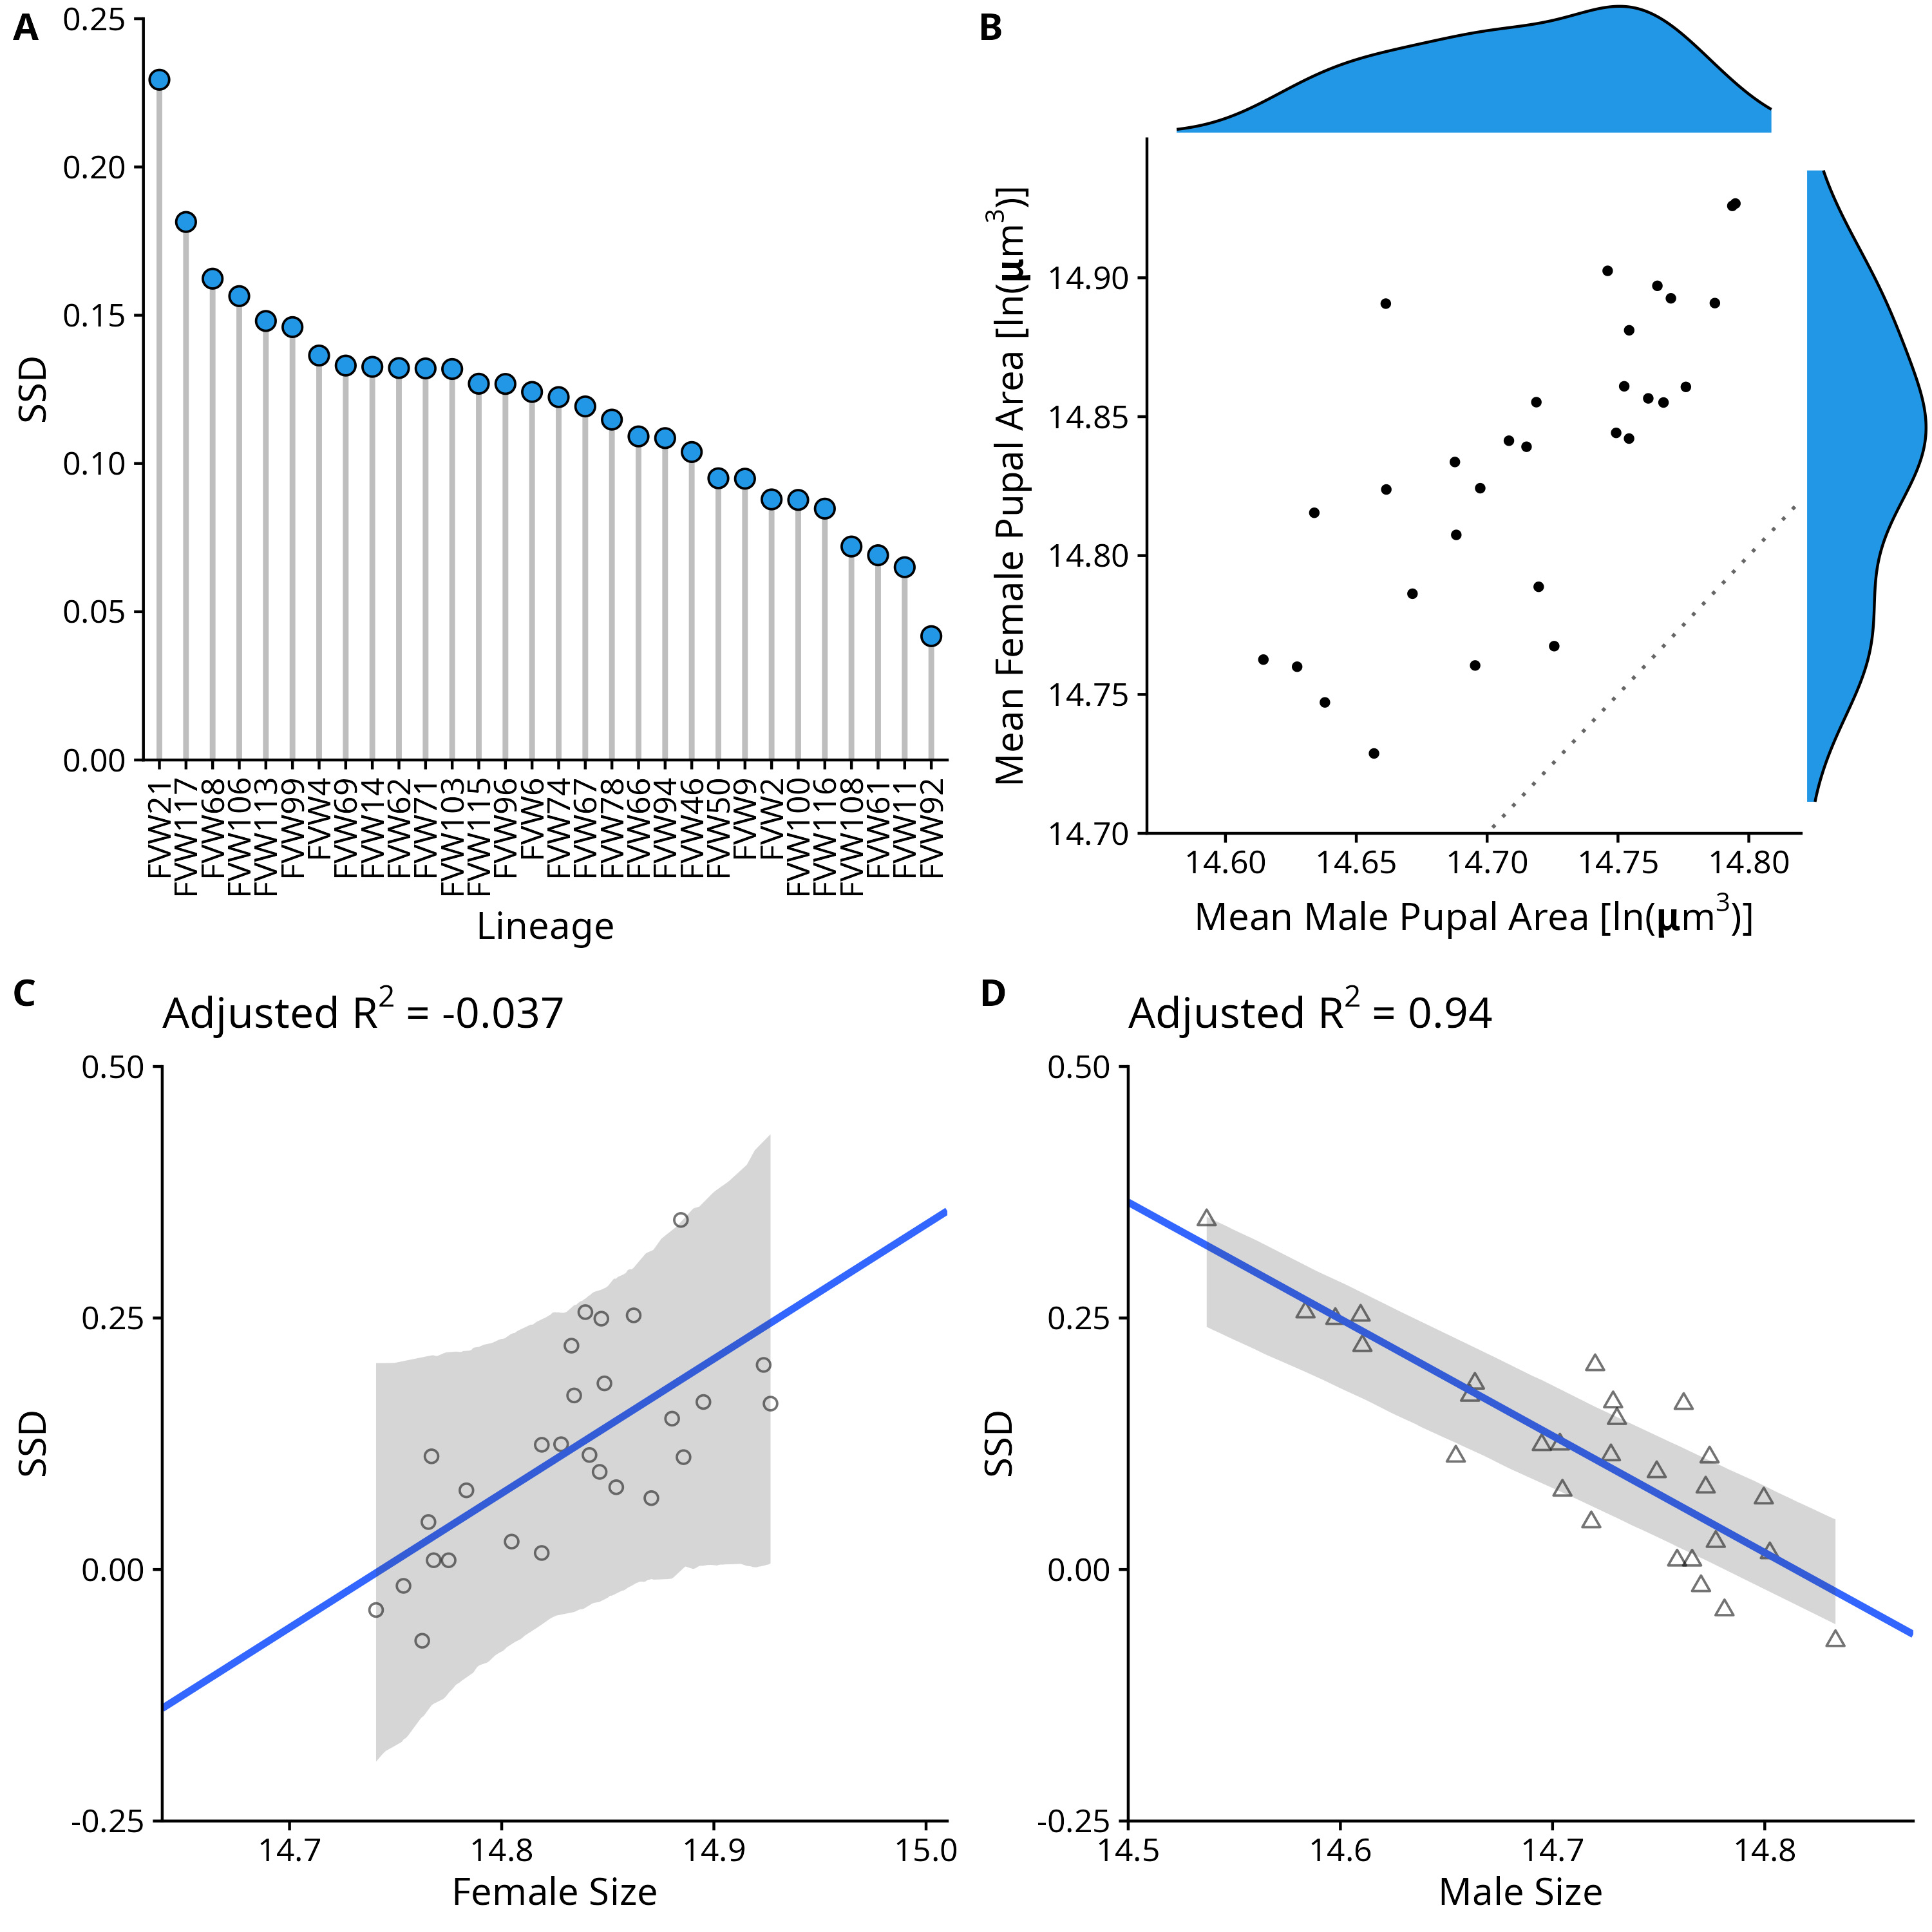
\includegraphics[alt = "Four graphs showing isogenized Fenn Valley Winery stocks have variation in sexual size dimorphism.", width=1\linewidth]{FVW_R2.png}
    \caption{SSD of FVW lineages is correlated with male body size. (A) SSD is highly variable between isogenized FVW lineages. (B) Both female and male body size vary substantially across lineages; the dotted line represents x = y, so SSD is the distance from this line. (C) SSD is not correlated with female size (adjusted \(R^2\) = -0.037), but (D) SSD is strongly correlated with male size (adjusted \(R^2\) = 0.94). These patterns indicate that variation in SSD among FVW lineages is primarily driven by variation in male body size.}
    \label{fig:FVW_R2}
\end{figure}

\subsection{Artificial Selection Changed SSD}

By generation 15, the bootstrapped credibility intervals for SSD in both the HL and LL no longer overlapped with the control lineage, indicating that selection was effective (\textbf{Figure 4A}). Changes in SSD were a result of changes in female and male body size. Female size increased in both the HL and LL relative to controls (\textbf{Figure 4B}). Conversely, LL males increased in size under selection and HL males remained similar in size to CL males despite the pressure to reduce in size (\textbf{Figure 4C}). Thus, the divergence in SSD was driven primarily by changes in male size, not female size.

\begin{figure}[t!]
    \centering
    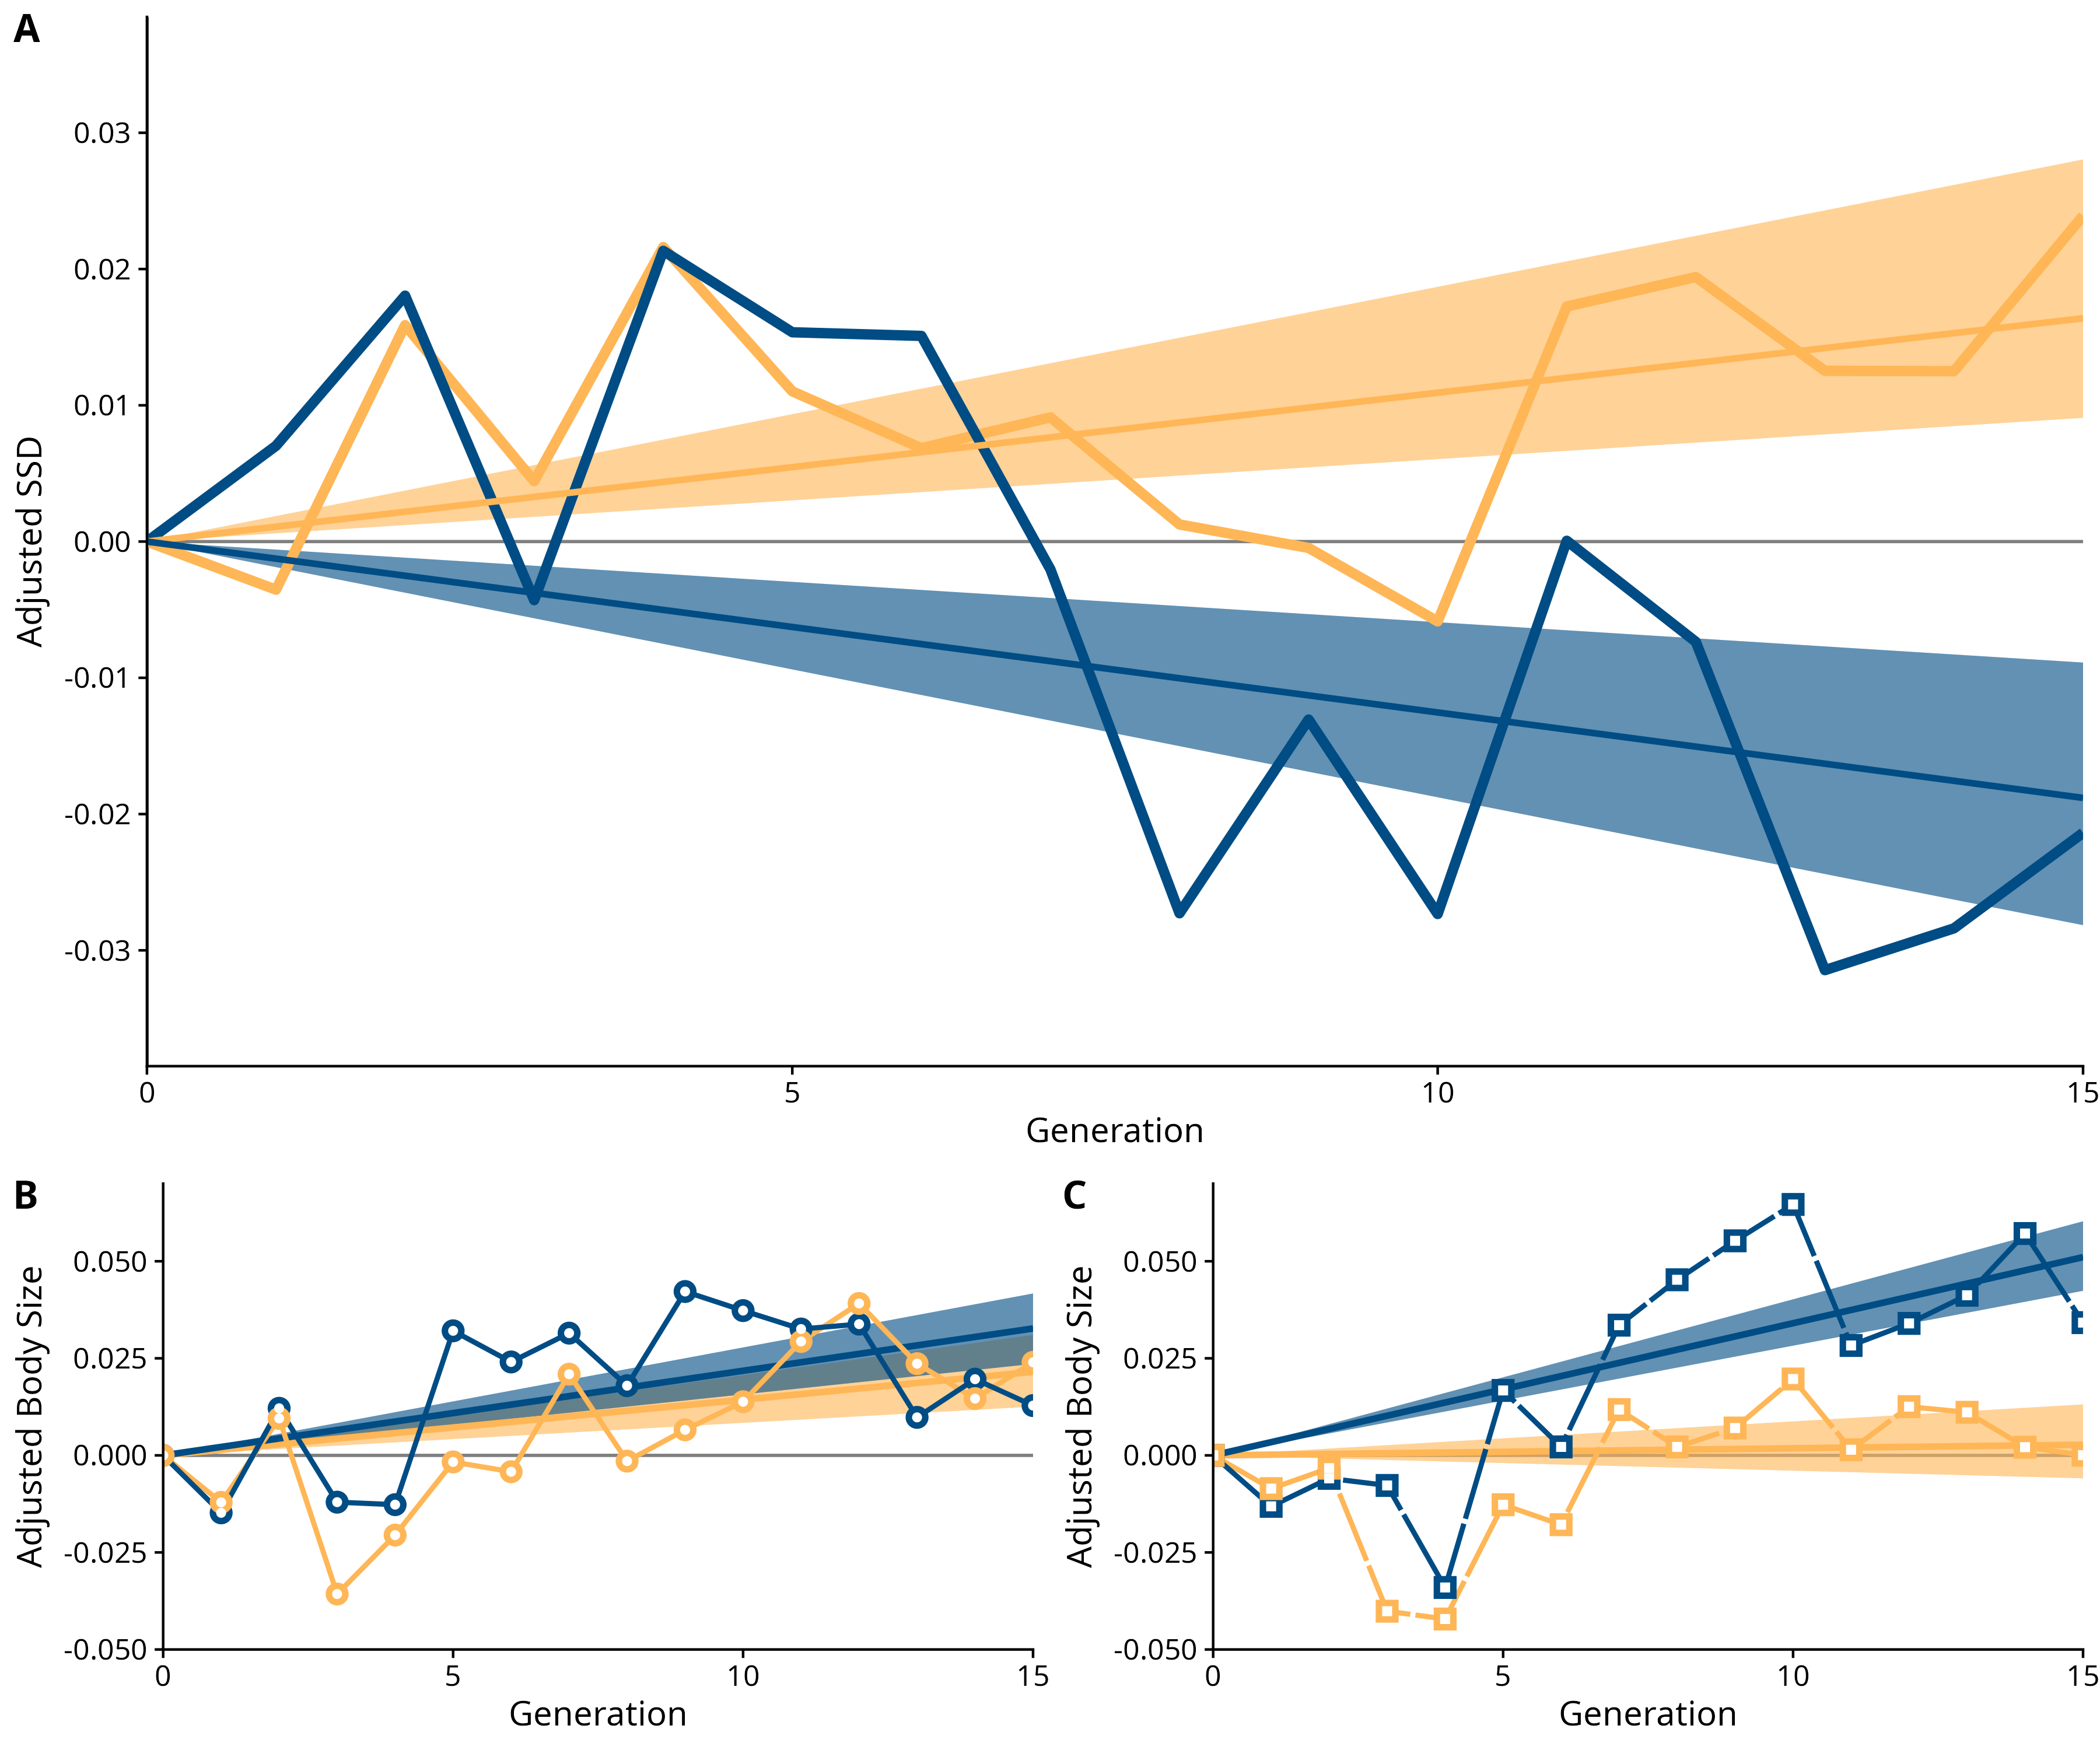
\includegraphics[alt = "Graphs showing selected lineages' diverged in regard to sexual size dimorphism.", width=1\textwidth]{fig2.1.png}
    \caption{SSD diverged from controls after only 15 generations of artificial selection. Responses are adjusted around the control lineage means. Shaded ribbons represent 95\% confidence intervals generated by bootstrapping (1000 resamples). (A) SSD divergence among lineages: both high SSD lineage (HL) and low SSD lineage (LL) no longer overlap with the control lineage (CL) by generation 15, indicating effective selection. (B) Female size increased in both selected lineages. (C) Male size differed significantly between selected lineages in response to selection, HL males body size remained similar to controls while LL male body size increased, thus SSD divergence was driven primarily by changes in male size.}
    \label{fig:generationalSSD}
\end{figure}

\begin{figure}[p]
    \centering
    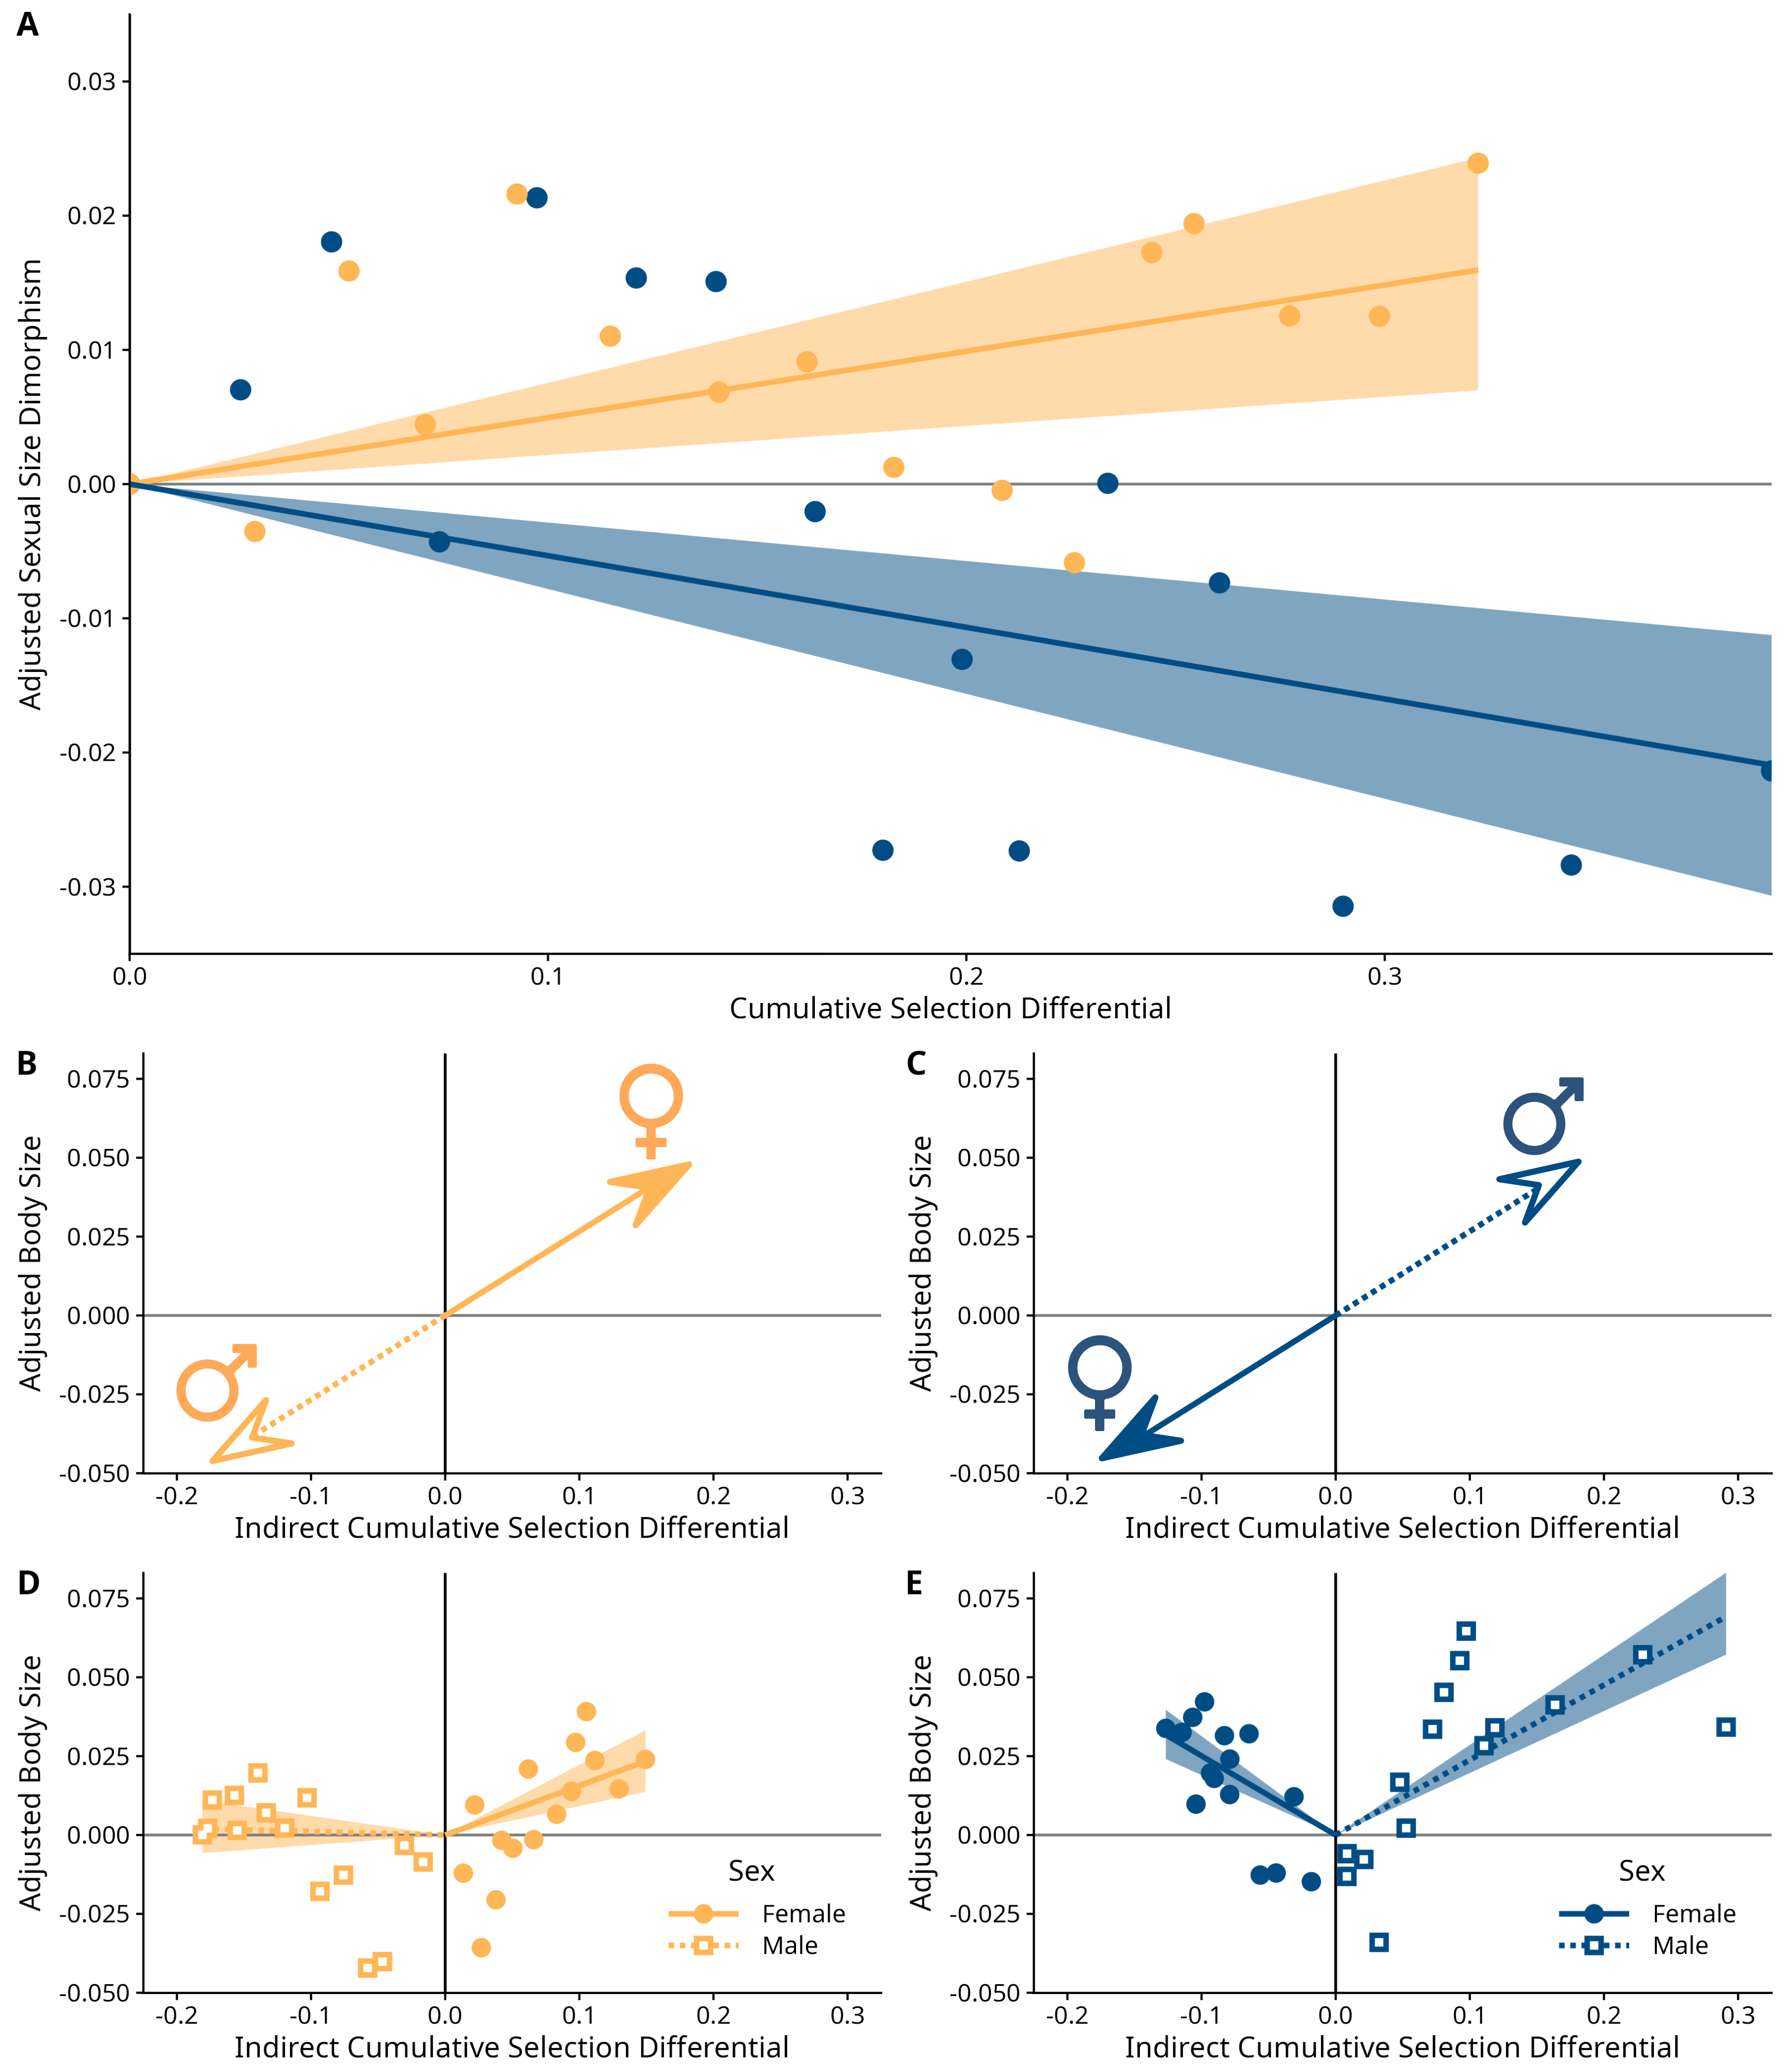
\includegraphics[alt = "Cumulative selection differentials showing that selection for sex specific reduced body size was constrained.", width=0.85\textwidth]{CSDfig.png}
    \caption{Adjusted cumulative selection differentials (CSD) over 15 generations. (A) CSD per lineage; positive represents selection for increased SSD (HL), negative represents selection decreased SSD (LL). (B–E) Left of origin reflects selection for smaller size; right reflects selection for larger size. (B–C) Expected indirect selection by sex: HL (B) selected for larger females and smaller males; LL (C) for smaller females and larger males. (D–E) Actual responses as deviation from control means. Shaded ribbons = 95\% CI (1,000 bootstrap resamples). In HL (D), female size increased with ICSD while males remained near controls despite selection for decrease. In LL (E), both sexes increased despite selection for reduced female size; LL males drove the SSD decrease with the largest ICSD and response of any group.}
    \label{fig:generationalSDs}
\end{figure}

To understand the selective pressures that produced the divergence in SSD, I calculated cumulative selection differentials (CSD) for each lineage. Selection differentials were calculated as the difference between the mean of the total population and the mean of the selected population, with the CSD being the sum total of these. Both HL and LL responded consistent with selection, with the HL experiencing an increase in SSD and LL experiencing a decrease in SSD (\textbf{Figure 5A}). Realized heritability was estimated from the cumulative response to selection across 15 generations. Increased SSD was more heritable than decreased (HL adjusted, where 'adjusted' refers to control-standardized values, \(h^2\) = 0.074; LL adjusted \(h^2\) = 0.055). These responses can be explored further by looking at the effects of selection on female and male body size.

\subsection{Selection Acted Asymmetrically on the Sexes} 

My selection regime targeted SSD, which necessarily imposed indirect selection on female and male body size. To quantify this, I calculated indirect cumulative selection differentials (ICSDs), which reflect the selective pressures applied to each sex indirectly. As SSD is female-biased (Testa et al., 2013; Vea et al., 2023), increasing SSD in the HL indirectly selected for larger females and smaller males, while decreasing SSD in the LL required selecting for smaller females and larger males. Thus if the sexes responded independently, the responses to selection would be in opposing directions (\textbf{Figures 5B and 2.5C}). This is not what I observed.

In the HL, females responded to selection for increased size (\(h^2\) = 0.16), while males experienced selection for reduced size but showed no detectable response (\(h^2\) = -0.0003) (\textbf{Figure 5D}). In the LL, females experienced selection for reduced size, yet size increased similarly to the HL females (\(h^2\) = -0.16) (\textbf{Figure 5E}), and the male response was consistent with selection on increasing male size (\(h^2\) = 0.11). Notably, while LL male size did not have the highest realized heritability, LL male size had the highest ICSD and response.

\subsection{Low Levels of Inbreeding Occurred}

Artificial selection inherently imposes a degree of inbreeding on the population as it restricts the number of breeding individuals each generation. Because inbreeding negatively affects the heritability of growth-related traits (Breden \& Wade, 1981; Sanchez et al., 1998; Wade et al., 1996) and viability (Amanullah et al., 2023), I calculated the inbreeding coefficient for each generation to provide insight into heritability, and to assess whether our relaxed selection protocols for generations 5, 10, and 15 saw any decline in the degree of inbreeding. 

\begin{figure}[!ht]
    \centering
    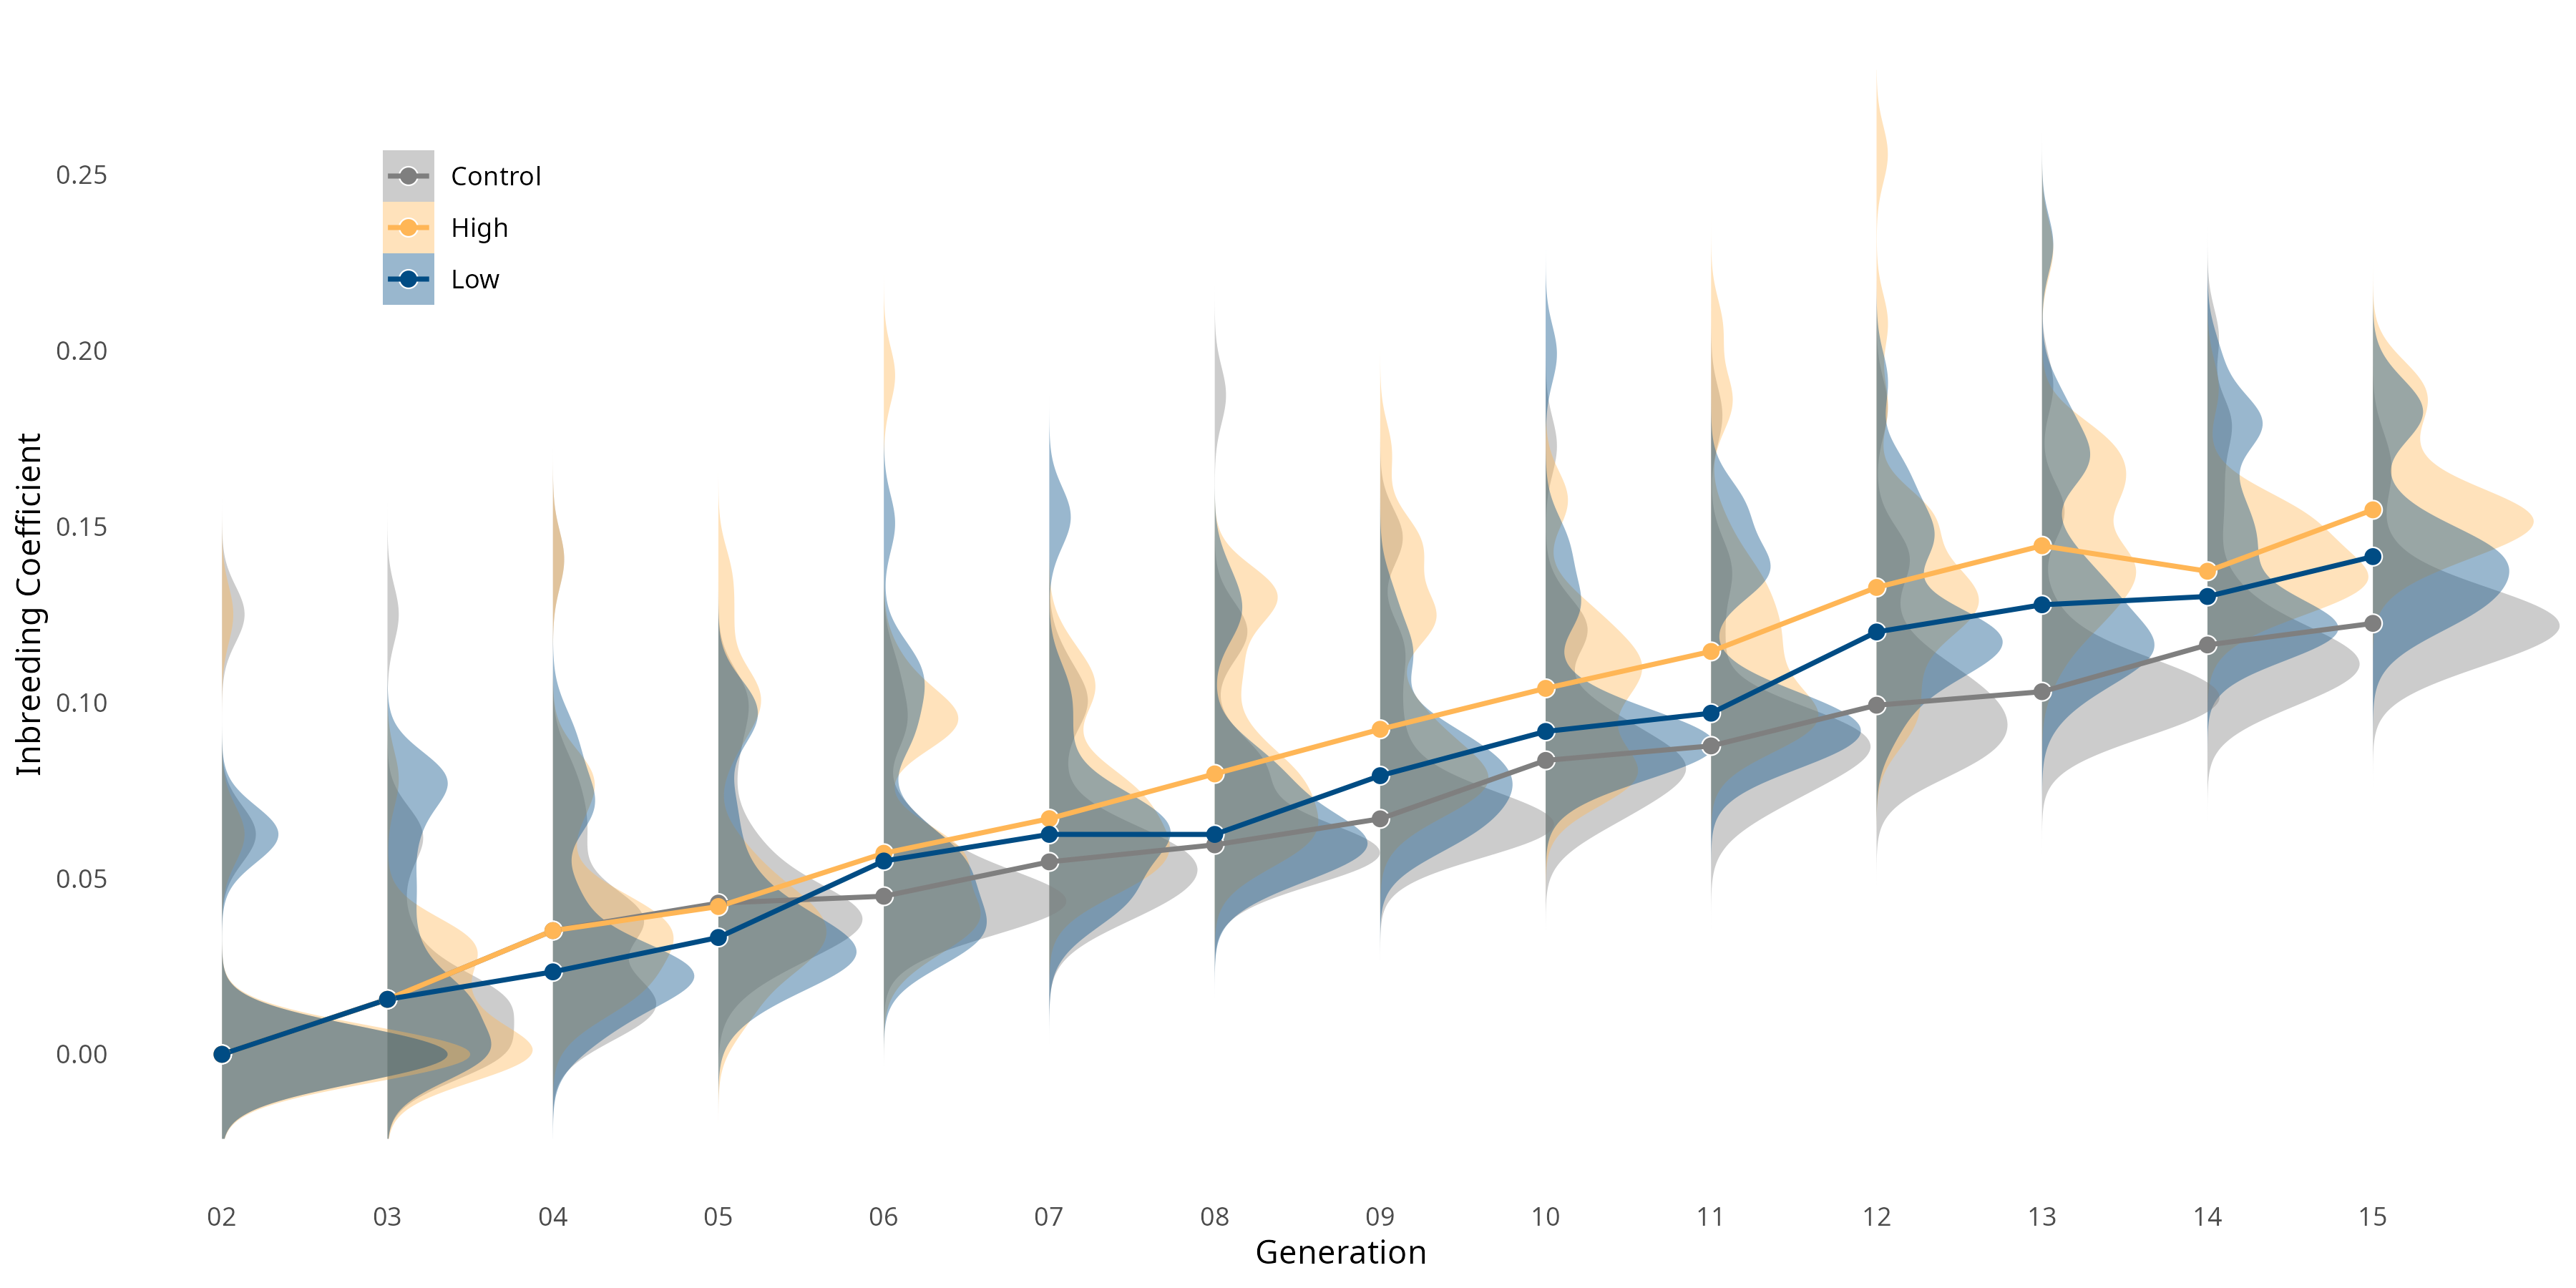
\includegraphics[alt = "Inbreeding coefficients remained low.", width=1\textwidth]{inbreed_coef.png}
    \caption{Inbreeding coefficients across 15 generations remained low. Inbreeding coefficients rose steadily in all lineages, including controls, with all lineages near 12.5\% by generation 15 which is equivalent to a single generation of first-cousin inbreeding. Selected lineages differ significantly from controls (GLM, $P$ < 0.001). Relaxed selection at generations 5, 10, and 15 did not slow the accumulation of inbreeding.}
    \label{fig:inbreed}
\end{figure}

Inbreeding coefficients rose steadily each generation among all lines (\textbf{Figure 6}). I expected relaxed selection at generations 5, 10, and 15 to slow the increase of the inbreeding coefficients, but it did not seem to have any impact. Towards the end of selection, all lineages, including the CL, had a median inbreeding coefficient over 12.5\%. An inbreeding coefficient of 12.5\% is equivalent to a single generation of first cousin inbreeding (Wright, 1922). Inbreeding coefficients were compared between lineages using a generalized linear model forced through zero at generation 1, as generation 2 was the earliest point at which inbreeding could occur given the experimental design. Both the HL and LL differed significantly from the CL ($P$ < 0.001). 

\section{Discussion}

The goal of this experiment was to use artificial selection to alter SSD, as part of an E\&R study focused on identifying the developmental-genetic mechanisms that underlie SSD expression and evolution.  After only 15 generations of family selection, I successfully diverged sexual size dimorphism (SSD) between the high SSD lineage (HL) and the low SSD lineage (LL), relative to control. This E\&R study contrasts with previous artificial experiments to change SSD because I selected directly on SSD using family selection rather than imposed discordant selection male and female body size at a population level (Stewart \& Rice, 2018; Tigreros \& Lewis, 2011). These earlier works either failed to change SSD (Tigreros \& Lewis 2011) or required more than 100 generations to see a response (Stewart \& Rice, 2018).

\subsection{Effect of Selection on SSD on Male and Female Body Size}

My artificial selection regime for changes in SSD was directed on the difference between male and female body size, but not directly on body size itself. The HL and LL saw changes in SSD because the response to selection differed between females and males. In both HL and LL lines, female body size increased similarly, and more than the control lineage (\textbf{Figure 4B}). In the HL, male body size did not increase more than control, thus resulting in an increase in SSD (\textbf{Figure 4C}). In the LL, however, male body size increased more than control and more than LL females, resulting in a decrease in SSD (\textbf{Figure 4C}). Thus the difference in response between the HL and LL lineages is due to the effects of artificial selection on male body size. 

The observation that changes in SSD between the HL and LL lineages were due to the male response to selection is consistent with the characterization of the FVW isogenized lineages, from the progenitive population. Among these lineages, male body size showed greater genetic variance than female body size, and SSD is correlated more strongly with male body size than female body size (\textbf{Figure 3)}. Thus we may \textit{a priori} expect selection on SSD to target male body size more than female body size. 

\subsection{Intralocus Sexual Conflict (IASC) and the Evolution of SSD}

The realized heritability of SSD was low, HL (\(h^2\) = 0.074) and LL (\(h^2\) = 0.055). This contrasts starkly with previous artificial selection experiments on different aspects of body size, which range from 0.2-0.4 in \textit{D. melanogaster} and in animals more broadly (Baptist \& Robertson, 1976; Flisar et al., 2014).  There are a number of mechanisms that can reduce realized heritability in artificial selection experiments, (eg high levels of inbreeding and reduced additive genetic variance), which we do not appear to see. Reduced fitness can also have an effect, (which I address later). However, a really critical factor in this case is intralocus sexual conflict (IASC).

My selection regime revealed signs of sexual conflict, the evolutionary tug-of-war that arises when traits have different fitness optima in females and males (Bonduriansky \& Chenoweth, 2009; Lande, 1980; Sayadi et al., 2019). Though a high realized intersexual genetic correlation (realized \(r_{MF}\)=0.76) was observed, suggesting that male and female body size are genetically coupled, my selection regime nonetheless diverged SSD. Because males and females share the vast majority of the genome (Mank, 2017; Price et al., 2023), genetic variants underlying body size are likely to have correlated effects in both sexes (Bonduriansky \& Chenoweth, 2009; Fisher, 1958; Lande, 1980). Under my selection regime, indirect selection was sexually antagonistic (imposed in opposite directions on the sexes): larger females with smaller males for the HL, and smaller females with larger males for the LL. Sexually antagonistic selection facilitates the most intense form of IASC, where selection on one sex displaces the other from its phenotypic optimum (Kasimatis et al., 2017).

If the sexes responded to selection independently, female and male body sizes would move in opposite directions relative to their respective selection pressures, placing them in opposing quadrants (\textbf{Figures 2.5B and 2.5C}). Instead, I observed patterns consistent with IASC. Sexual conflict was most clearly seen in the LL: despite indirect selection for reduced female size, female body size increased relative to controls. A similar phenomenon occurred in the HL: despite indirect selection for reduced male size, male body size did not deviate from controls at the end of selection. That HL males are in the quadrant adjacent to HL females, and LL females adjacent to LL males, indicates that selection on one sex generated a correlated response in the other--a signature of IASC constraining sex-specific responses (Mank, 2017; Price et al., 2023). Tigreros and Lewis (2011) observed similar phenotypic constraints, as the sexes experienced parallel changes in size despite discordant selection. Thus, the rapid evolution observed here suggests that family selection on sexually antagonistic phenotypes can mitigate, but not eliminate, the constraints of sexual conflict.

Previous studies have used the maintenance of multiple alleles to infer sexual conflict and their results suggest that a substantial portion of the genome is under sexual conflict and that this maintenance may constrain the evolution of sexual dimorphism (Ostrowski et al., 2015; Mank, 2018). However, a limitation of my E\&R study is that standard methods of genomic sexual conflict, such as comparing Tajima's D to \(F_{ST}\), are not appropriate for my lineages. The single-pair mating and family selection employed repeatedly bottleneck the populations, which violates the assumptions of such analyses (Kasimatis et al., 2017; Wright et al., 2018). I therefore considered alternative explanations for the observed responses to selection.

There are other non-exclusive explanations as to why males or females  did not respond to indirect selection on body size. In HL line, males did not decrease body size in response to (indirect) selection \(h^2 = -0.003\). It is possible that this is because there is a lower limit to male body size, below which they become nonviable. This cannot be the case as HL males were smaller in previous generations (\textbf{Supplementary Figure 3}).

Conversely, in the LL lines, female body size did not decrease in response to (indirect) selection to do so \(h^2 = -0.16\). In contrast, they showed an increase in body size. While this may a consequence of IASC, it is also possible that my selection regime imposed additional positive directional selection on female body size via fecundity selection (Amanullah et al., 2023; Lefranc \& Bundgaard, 2000). This would have occurred after females had been selected for body size. If this were true, then you would expect larger females to produce more offspring. However, my data do not support this hypothesis. I compared the average familial female size of females that successfully produced the minimum number of offspring required to be considered for selection to those that did not via a binomial generalized linear model and found that there was no difference in size ($P$ = 0.29). This suggests maternal family size did not effect the likelihood of producing enough offspring to meet regime minimums. Consequently, the most parsimonious explanation for the opposing effects of selection and response on male and female body size is IASC.

\subsection{Future Directions}

The primary limitation of this E\&R experiment is the absence of replicate selected lineages, which complicates the definitive attribution of allele frequency changes to selection rather than drift. To address this, I will compare the loci that responded to selection in my divergent lineages with the 110 candidate genes identified by Vea et al.'s (2026) GWAS. Intersecting loci are unlikely to arise by chance and therefore represent high-confidence candidates for regulating SSD. The phenotypic divergence documented here provides the foundation for two complementary lines of inquiry: first, genomic analysis (which I will present in Chapter 3), and second, characterization of causative traits underlying SSD using isogenized derivatives of these lineages (which I will present in Chapter 4).

\section{Conclusion}

To conclude, I found that SSD is an evolvable trait that responds rapidly to artificial selection. The divergence in SSD was driven primarily by changes in male body size, reflecting the greater standing genetic variation in male size within the FVW population. Asymmetric responses between the sexes are best explained by intralocus sexual conflict constraining the evolution of SSD. In the following chapters, I use these lineages for genomic analysis (Chapter 3) and to explore traits correlated with SSD, such as minimal viable weight and fecundity (Chapter 4).

\newpage
\chapter{Genetic Comparisons of Resulting Populations}

The difference between male and female body size (sexual size dimorphism, SSD), is one of the most obvious ways in which the sexes differ. In \textit{Drosophila melanogaster}, as in most arthropods, females are the larger sex (Testa et al., 2013; Vea et al., 2026; Webb \& Freckleton, 2007). Research over the last thirty years has established the developmental, genetic, and physiological mechanisms that regulate body size, much of which has been done in \textit{D. melanogaster}. It is well understood that females and males share the vast majority of the genome and that sex determination leads to differences in gene expression, which ultimately generate SSD (Lande, 1980; Bonduriansky \& Chenoweth, 2009; Sayadi et al., 2019). However, while sex determination and the selective pressures that produce observed patterns of SSD have been well studied, how SSD occurs at the developmental-genetic level remains largely unknown.

A widely used approach to identify the genetic basis of a quantitative phenotype is the genome wide association study (GWAS) (Visscher et al., 2012), which compares variation in phenotype and genotype across existing populations to identify candidate genes associated with the trait of interest (Visscher et al., 2012; Tam et al., 2019). A complementary approach to identify the genetic basis of a quantitative phenotype is the Evolve and Resequence (E\&R) study, which increases the frequency of causative alleles by using artificial selection to drive phenotypic change. Loci that respond to selection are identified by comparing genomes of selected and unselected populations (Vlachos \& Kofler, 2019). E\&R not only identifies the genes associated with trait of interest, however, but also provides insight into how the trait of interest responds to selection. In combination, therefore, GWAS identifies the loci that underlie standing genetic variation for a trait, while E\&R identifies which of these loci are targeted by selection to generate phenotypic change in the trait of interest. GWAS and E\&R are complementary approaches and have been used in combination to successfully identify the genes underlying \textit{D. melanogaster} courtship song (Turner et al., 2013).

Here I use E\&R as a complementary approach to a previous GWAS to (1) identify the developmental-genetic mechanisms that regulate SSD in \textit{D. melanogaster} and (2) explore which aspects of these mechanisms can be targeted by selection to generate evolved changes in SSD. The previous GWAS not only established that there is ample standing genetic variation in SSD in \textit{D. melanogaster}, but also identified 110 loci associated with this variation. Intriguingly, almost none of these loci lay within genes previously characterized as regulators of SSD, specifically genes involved in the nutritional regulation of body size (Testa, 2013; Vea et al. 2026). Body size is, however, a very large genetic genetic target and is impacted by myriad genes. The results of the GWAS are perhaps, therefore, not unexpected. What is unclear is whether selection on SSD  targets the subset of these loci specifically involved in the nutritional regulation of body size, as implied developmental studies on SSD (Rideout et al., 2015; Testa et al., 2013). 

Chapter 2 described the successful divergence of SSD in \textit{D. melanogaster} through 15 generations of family selection. The resulting lineages consist of a high SSD lineage (HL), a low SSD lineage (LL), and a control lineage (CL). In this chapter, I describe the "resequence" portion of my E\&R study. I compare allele frequencies between my initial population from the Fenn Valley Winery (FVW) stock with generation 15 of the resulting lineages. By identifying loci with significant changes in allele frequency in selected lineages, I identified regions that responded to selection. The identified regions were then compared with the 110 GWAS hits associated with SSD identified by Vea et al. (2025). Overlapping loci represent high-confidence candidates for regulating SSD. Furthermore, I examined whether these candidate genes have functions in known growth-regulating pathways, particularly the insulin/IGF signaling pathway (IIS) that has been shown to be necessary for SSD (Carreira et al., 2009; Testa et al., 2013; Rideout et al., 2015). This exploration will tell me which genes likely regulate SSD and whether those genes are involved in the canonical IIS pathway.

\section{Methods}
All statistical analyses were conducted in R. Code and data are available on GitHub at \url{https://github.com/LizAgolli/Resequence-SSD}

\subsection{Sample Preparation}

The parents of generations 0 and 15 were stored at -80°C. Generation 0 parents were separated by sex, with each sex having five pools of 24 individuals. For the evolved lineages, the populations were separated by sex into four pools of no more than 25 individuals (see supplementary \textbf{Table 1} for pool count data). Library preparation and sequencing were performed by The Genome Access Technology Center at the McDonnell Genome Institute at Washington University. Library preparation was performed using the WGS KAPA Hyper PCR-free kit and sequencing was done with Nova-SeqX.

\subsection{Bioinformatics Pipeline}

We followed the Audet et al. (2024) pipeline, with only minor deviations to make use of more recent program versions and adjust for the details of our study design. The raw reads were trimmed using bbduk v39.13 (Bushnell, 2021) and aligned with BWA-mem v0.7.18 (Li, 2013) to the \textit{D. melanogaster} reference genome v6.62 (FlyBase release FB2026\_01). SAMtools v1.16.1 (Li et al., 2009) was then used to convert the resulting Sequence Alignment Map (SAM) files to Binary Alignment Map (BAM) files to merge read groups. BAM files were merged by line for between line comparisons and by both line and sex for sex-specific comparisons. A blacklist was generated by combining known transposable elements from the reference genome dmel-6.62 and the problematic regions identified by Amemiya et al. (2019). Repeats and the blacklisted sites were filtered using Repeatmasker v4 (Smit et al., 2013-2015) and Popoolation v1.2.2 (Kofler et al., 2011). We then used Grenedalf v0.6.3 (Czech et al., 2024) to calculate \(F_{ST}\). Bioinformatics was done on the University of Illinois Chicago Lakeshore HPC Cluster servers.

\section{Statistical Methods}

To detect which variants changed in frequency as a result of selection, I utilized an adapted chi-squared test designed to account for the unique challenges of E\&R experiments, including genetic drift due to finite population size and sampling variance from pool sequencing (Spitzer et al., 2019).

To account for genetic drift, the analysis utilizes the effective population size \(N_e\). This was calculated as 

\[N_e = \frac{N}{1 + Q^2C^2}\]

\noindent where \(Q^2\) the effect of selection (and can be estimated as \textit{Q} = 2 if loci are assumed to be unlinked) and \(C^2\) is the variance of the trait under selection as suggested by Wang et al. (2016) for selection experiments.

\subsection{Adapted Chi-squared Test} 

To identify where changes in allele frequency occurred as a result of selection, the adapted chi-squared test was conducted using the ACER R package (Spitzer et al., 2019). This test was specifically adapted to account for the overdispersion of loci, and in doing so is more effective at identifying true positives compared to a standard chi-squared analysis. This approach is computationally efficient and does not require replicates, but does not provide explicit estimates of the selection coefficients. I applied the adapted chi-squared tests to three pairwise comparisons of allele frequencies at single base positions between: (1) the initial against CL (control), (2) the initial against HL, and (3) the initial against LL. The significance threshold was set to \(10^{-6}\), as is standard for genome wide studies (Fadista et al., 2016; Vea et al., 2026).

\subsection{Identifying Candidate Genes and Comparing to DGRP GWAS}

Genomic regions as defined by FlyBase (release FB2026\_01) corresponding to these candidate SNP locations were considered candidate genes. As CL were not selected upon, any genes flagged by the initial against CL chi-square test must be a result of genetic drift. As such, any genes flagged by the CL chi-square test were not considered candidate genes. The candidate genes identified by the chi-square analyses of the selected lineages were then compared to each other and to the candidate genes associated with SSD and SSP identified by the DGRP GWAS conducted by Vea et al. (2026). 

\subsection{Enrichment Analysis of Intersecting Candidate Genes}

GO and KEGG enrichment analyses were conducted using PANGEA (Hu et al., 2023) on two gene sets of high confidence: (1) genes that returned signals in both chi-squared analyses, and (2) genes that returned a signal in at least one chi-squared analysis and at least one of Vea et al.'s (2026) DGRP GWAS outputs (see \textbf{Table 2}). The first represents the highest-confidence subset from my E\&R having signaled in both selected lineages, and second set are high confidence as they signaled with different methods and populations.

\section{Results}

\begin{figure}[b]
    \centering
        \centering
        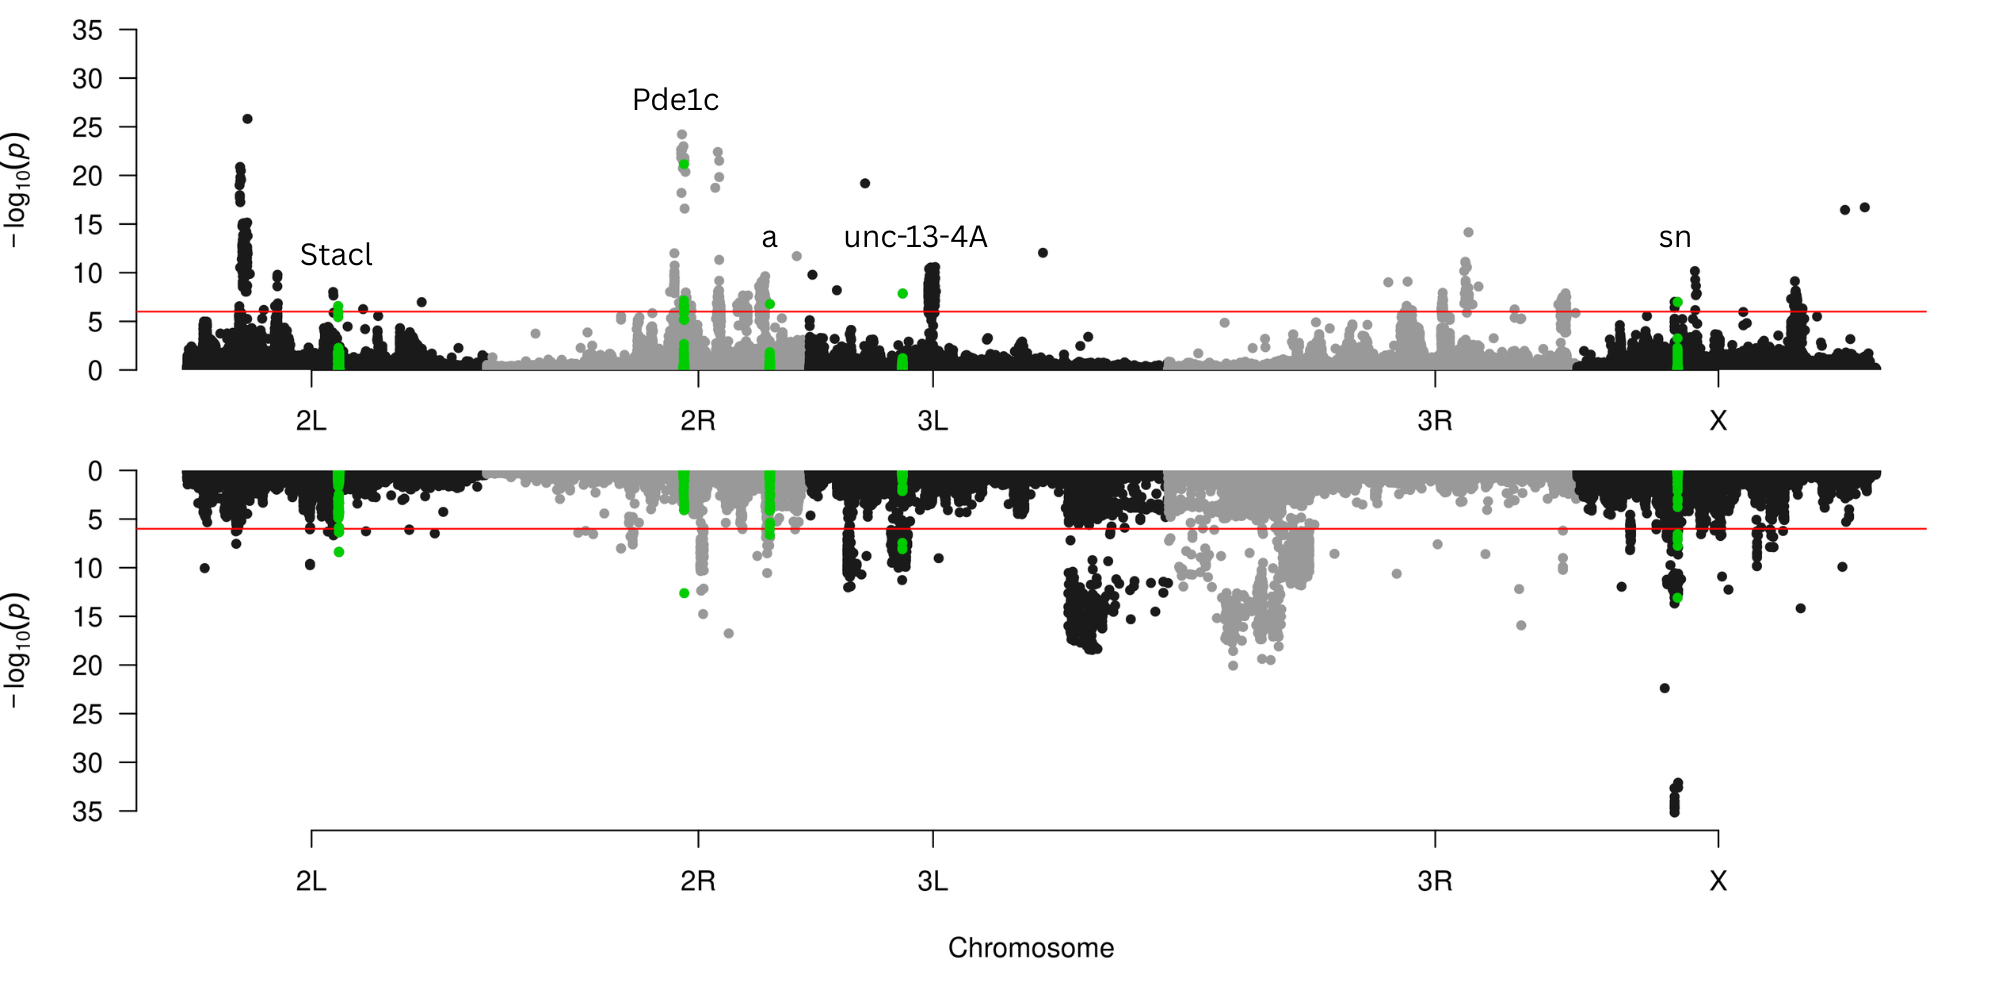
\includegraphics[alt = "Manhattan plots of adapted chi-square results showing five shared hits between HL and LL.", width=\linewidth]{bothChiHits.png}
        \caption{Manhattan plots of adapted chi-square results. Genes with significant allele frequency changes in both HL and LL, but not in CL, are highlighted. The upper panel shows HL results; the lower panel shows LL results. The horizontal lines indicate the significance threshold $P = 10^{-6}$. These intersecting candidate genes represent high-confidence candidates for SSD regulation.}
        \label{fig:chi_hits}
\end{figure}

\subsection{Adapted Chi-squared}

The adapted chi-squared test identified 192 HL genes and 319 LL genes as having SNPs with significant allele frequency changes. The asymmetry between these lineages could reflect genetic drift but might also reflect differences in genetic architecture underlying divergent SSD, though this warrants further investigation. Of these candidate genes, five genes are identified in both lists (\textbf{Table 1)}. In each case, the significant SNPs in HL and LL map to different positions within the gene, suggesting that distinct alleles at these loci can drive SSD in either direction.
%SHOULD I NOTE THE INVERSION FROM 3L AND 3R IN TEXT OR IN FIGURE CAPTION?

\subsection{Comparison with DGRP GWAS Points to \textit{unc-13-4A}}

Comparing my analyses to the Vea et al's (2026) DGRP GWAS results, of the 506 candidate genes identified by my adapted chi-square analysis, I identified 14/110 genes identified by Vea et al.'s (2026) DGRP GWAS for SSD and SSP. There are 13,986 known protein-coding genes on the \textit{D. melanogaster} genome (Mohr et al., 2023), therefore the likelihood of these separate methods identifying an overlap of this magnitude or greater is exceedingly small (\textit{$P$ < 0.001}). Among candidates from the HL chi-squared analysis, the LL chi-squared analysis, Vea et al.'s (2026) GWAS for SSD, and GWAS for SSP, \textit{unc-13-4A} emerges as the sole consistent candidate gene. 

\begin{figure}
    \centering
    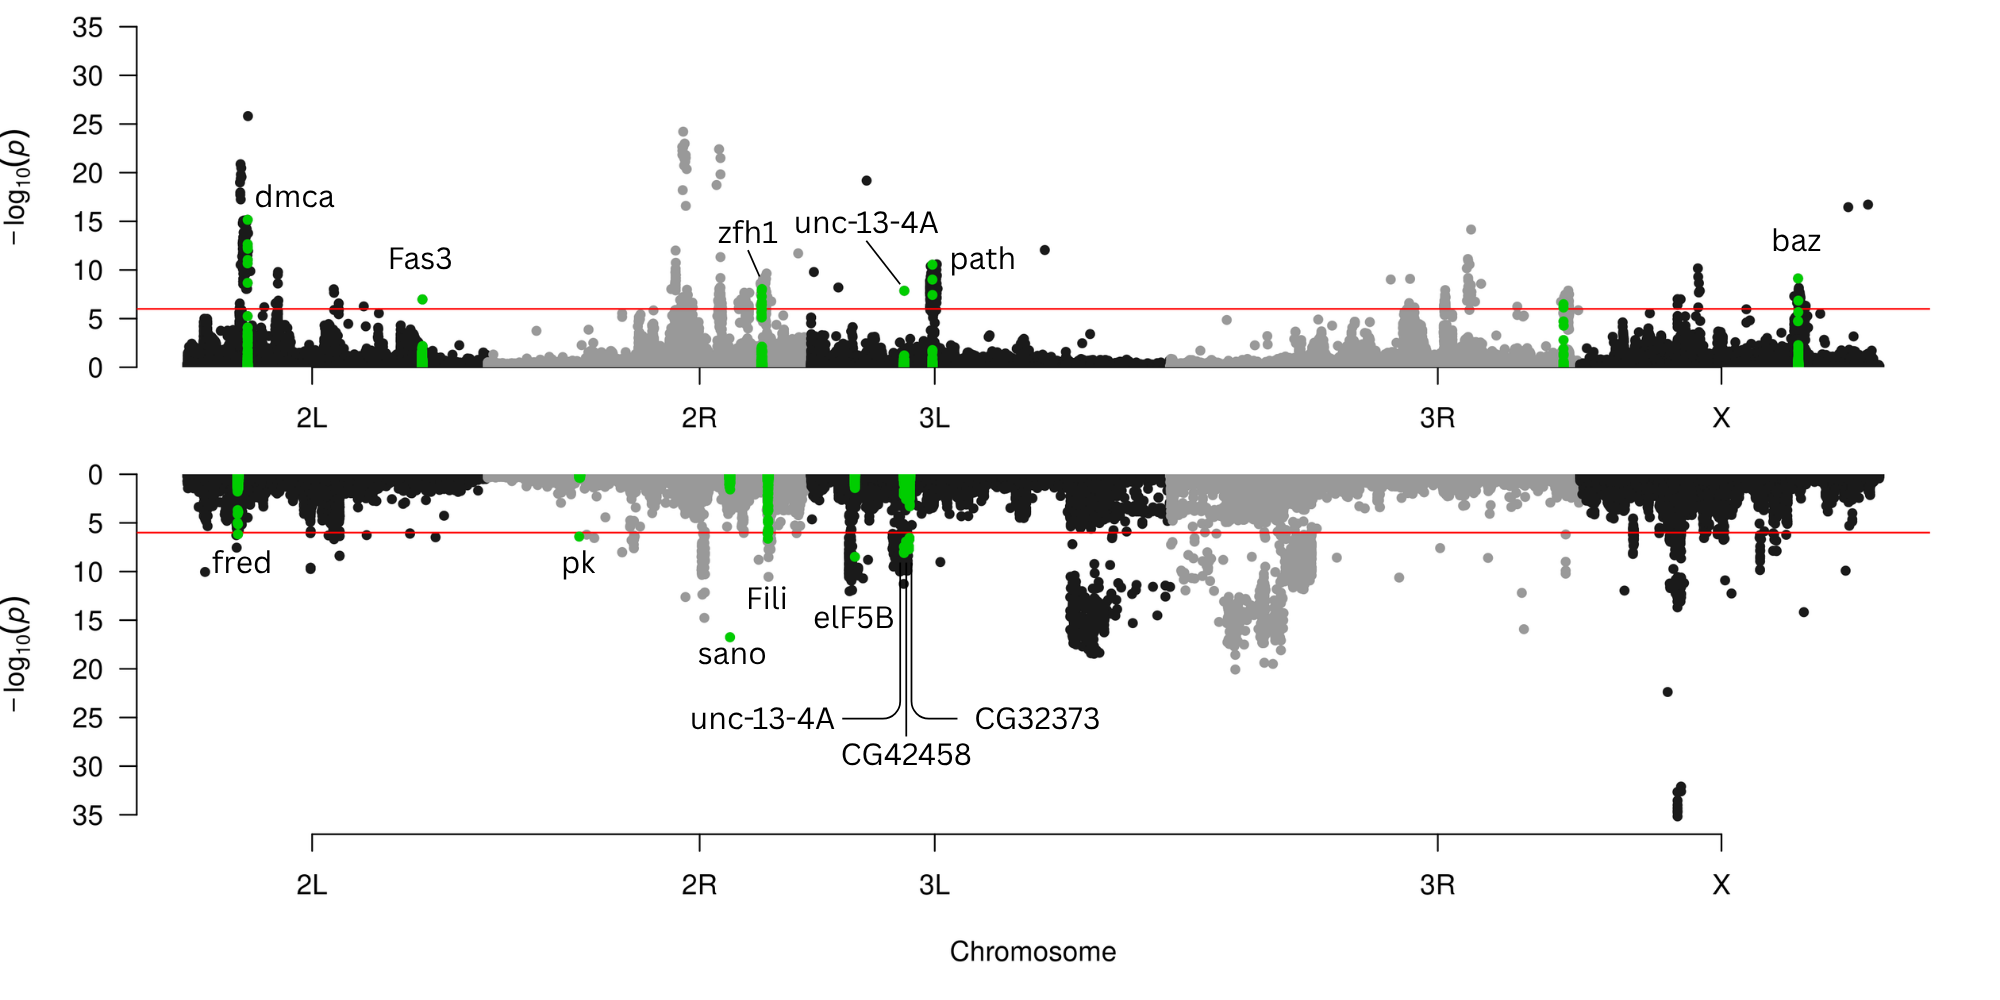
\includegraphics[alt = "Manhattan plots highlighting hits shared with Vea et al's 2026 DGRP GWAS.", width=1\linewidth]{manGWASandChi.png}
    \caption{Manhattan plots of adapted chi-square results highlighting genes with signals in both the respective selected lineage and Vea et al.'s (2026) GWAS, but not in CL. The upper panel shows HL results; the lower panel shows LL results. Highlighted genes (green) represent high-confidence candidates that responded to selection in my experiment and were also associated with SSD in an independent population (DGRP). The red lines indicate the significance threshold $P$ = 10e-6.}
    \label{fig:manGWASandChi}
\end{figure}

\begin{figure}
        \centering
        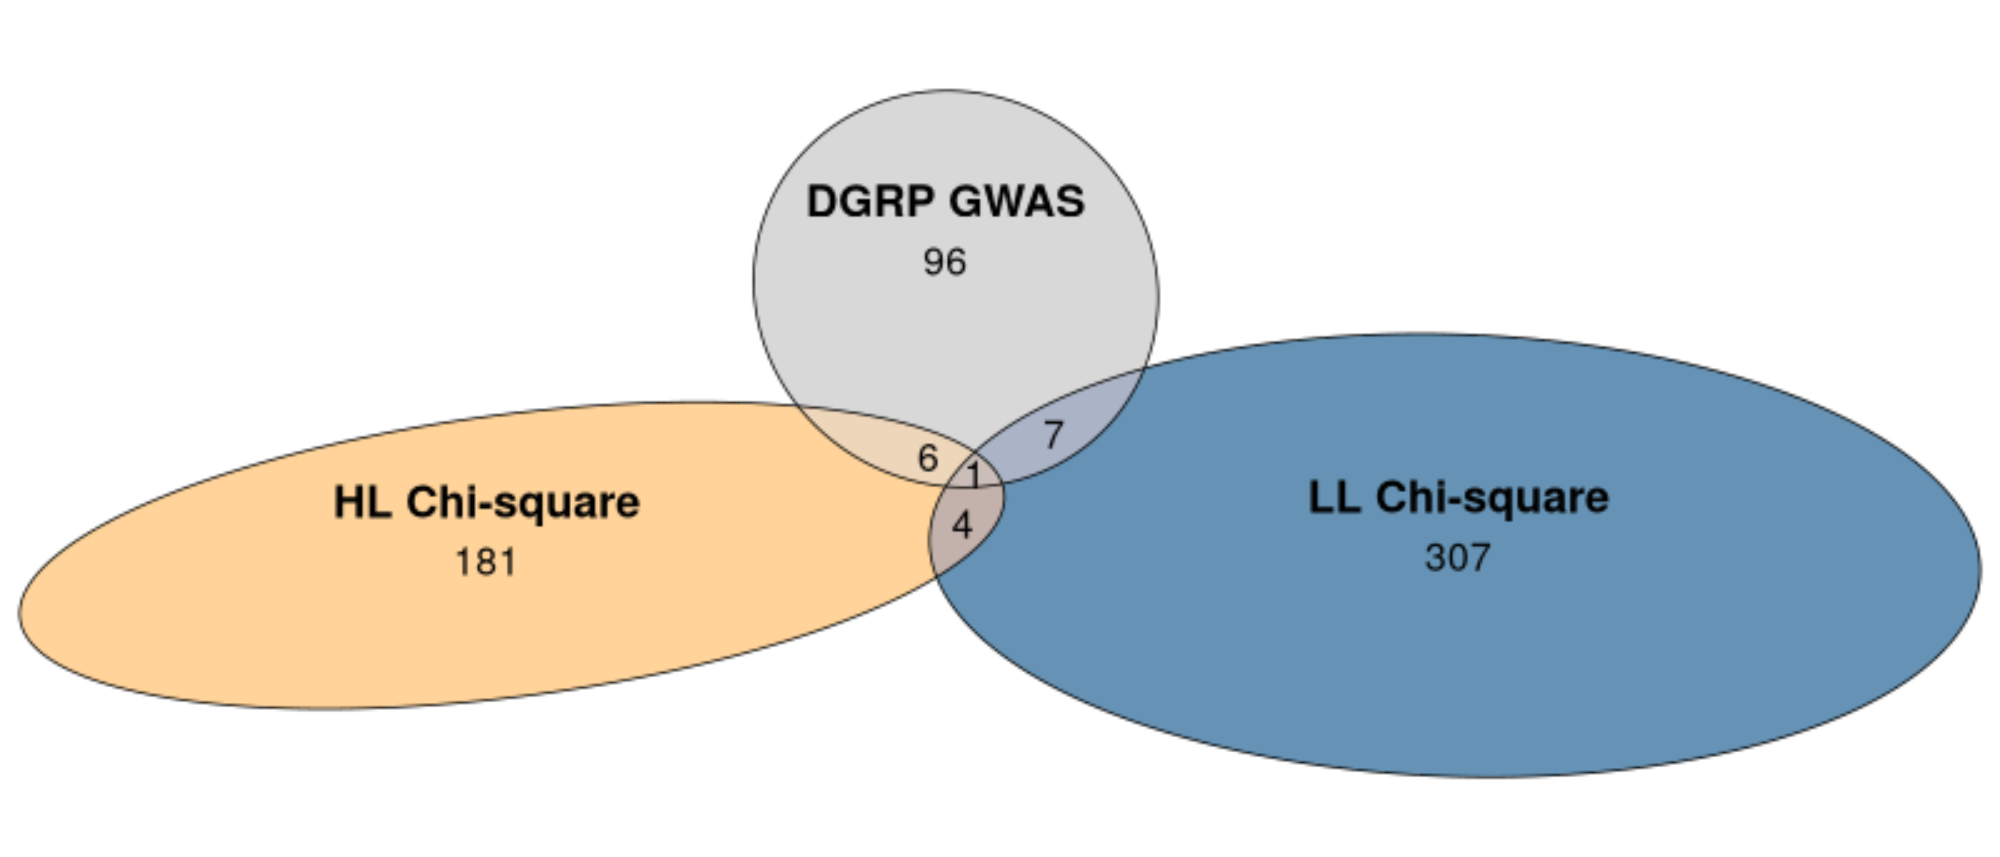
\includegraphics[alt = "Venn diagram of candidate genes.", width=1\linewidth]{vennElipseScale.png}
        \caption{Venn diagram of candidate genes identified by adapted chi-square tests and Vea et al.'s (2026) GWAS. Chi-square tests identified 192 candidate genes in HL and 319 in LL after filtering signals present in controls. Vea et al. (2026) identified 110 candidate genes associated with SSD and SSP in the DGRP. The overlap of 14 genes between my E\&R study and Vea et al.'s independent GWAS is highly significant (hypergeometric test, $P$ < 0.001), indicating that the selection regime successfully amplified biologically relevant alleles.}
        \label{fig:venn}
\end{figure}

\tagpdfsetup{table/header-rows={1}}
\begin{table}
    \caption{Genes that signaled more than once in chi-square tests and the GWAS of Vea et al. (2026).}
    \centering
    \begin{tabular}{rcccl}
        & \multicolumn{2}{c}{\(X^2\)} & & \\
        & \rotatebox{90}{High} & \rotatebox{90}{Low} & \rotatebox{90}{GWAS} & Function\\ \hline
        \textit{a}          & \(\bullet \)    & \(\bullet \) & & compound eye development \\ \hline
        \textit{baz}	    & \(\bullet \)	  & 	         & \(\bullet \) & axis elongation  \\  \hline
        \textit{CG32373}	&  	              & \(\bullet \) & \(\bullet \) & synaptic target recognition\\  \hline
        \textit{CG42458}	& 	              & \(\bullet \) & \(\bullet \) & RNA stabilization \\  \hline
        \textit{dcma}	    & \(\bullet \)	  &              & \(\bullet \) & G protein-coupled receptor signaling pathway \\  \hline
        \textit{eIF5B}	    &	              & \(\bullet \) & \(\bullet \) & translational initiation \\  \hline
        \textit{Fas3}	    & \(\bullet \)	  &              & \(\bullet \) & synaptic target recognition \\  \hline
        \textit{Fili}       &	              & \(\bullet \) & \(\bullet \) & regulation of apoptotic process \\  \hline
        \textit{fred}	    &  	              & \(\bullet \) & \(\bullet \) & compound eye morphogenesis \\  \hline
        \textit{path}	    & \(\bullet \)	  &              & \(\bullet \) & dendrite extension \\  \hline
        \textit{Pde1c}      & \(\bullet \)    & \(\bullet \) & & signal transduction, cGMP and cAMP metabolic process \\ \hline
        \textit{pk}	        & 	              & \(\bullet \) & \(\bullet \) & establishment of protein localization \\  \hline
        \textit{sano}	    & 	              & \(\bullet \) & \(\bullet \) & establishment of ommatidial planar polarity  \\  \hline
        \textit{Sdc}	    & \(\bullet \)	  & 	         & \(\bullet \) & axon guidance \\  \hline
        \textit{sn}         & \(\bullet \)    & \(\bullet \) & & microvillar actin bundle assembly and maintenance of cell polarity \\ \hline
        \textit{Stacl}      & \(\bullet \)    & \(\bullet \) & & calcium ion transmembrane transport \\ \hline
        \textit{unc-13-4A}  & \(\bullet \)    & \(\bullet \) & \(\bullet \) & synaptic vesicle priming and neurotransmitter secretion \\  \hline
        \textit{zfh1}	    & \(\bullet \)	  &              & \(\bullet \) & garland nephrocyte differentiation \\  \hline
            \end{tabular}
    \label{tab:hits}
\end{table}

\subsection{Intersecting Genes Enrich for Neurodevelopment and Polarity}

A GO analysis of the five highest-confidence candidate genes, those returning signals in both chi-square analyses (\textbf{Figure 1}), found high enrichment for developmental processes such as cell junction, sensory organ development, cellular localization, animal organ development, cellular component assembly, and system development. When candidate genes were expanded to include those with corroborating signals in Vea et al.'s (2026) DGRP GWAS (\textbf{Table 1}), the GO analysis of this set found high enrichment for neurodevelopmental terms, including neuron development, neuron differentiation, generation of neurons, and neurogenesis, as well as cell projection and axon-related processes such as neuron projection morphogenesis, axon guidance, axonogenesis, and axon development. Cell adhesion, junction, and polarity related terms were also enriched. Terms related to growth and size regulation were also detected, including developmental growth, regulation of anatomical structure size, and cell growth. A KEGG analysis showed the candidate genes are involved the Hippo signaling pathway, namely \textit{baz} and \textit{fred}.

\section{Discussion}

The goal of this experiment is find the loci where artificial selection targeted to alter SSD, as part of an E\&R study focused on identifying the developmental-genetic mechanisms that underlie SSD expression and evolution. After only 15 generations of family selection, I successfully diverged sexual size dimorphism (SSD) between the high SSD lineage (HL) and the low SSD lineage (LL), relative to control (see Chapter 2). This E\&R study contrasts with previous artificial experiments to change SSD because I selected directly on SSD using family selection rather than imposed discordant selection male and female body size at a population level (Stewart \& Rice, 2018; Tigeros \& Lewis, 2011). Candidate loci identified by my study should therefore be those directly involved in the regulation of SSD.

I identified genes that responded to divergent selection on SSD over 15 generations and compared these to a genome-wide association study (GWAS) using the \textit{Drosophila} Genetic Reference Panel (DGRP) conducted by Vea et al. (2026). The 14 genes identified by both my E\&R study and Vea et al.'s (2026) GWAS (\textbf{Table 2}) are unlikely to be due to random chance ($P$ < 0.001), suggesting the selection regime successfully amplified biologically relevant alleles and that these alleles are involved in the regulation of SSD.

\subsection{Absence of IIS Pathway Genes}

We have an increasingly good understanding of the developmental genetic mechanisms that regulate adult body size. In particular, work in \textit{Drosophila} over the past three decades has illuminated the critical role the insulin/insulin-like growth factor signaling (IIS) and Target of Rapamycin (TOR) pathways play in the regulation of growth and body size (Rideout et al., 2015; Testa et al., 2013; Texada et al., 2020;  Mirth \& Shingleton, 2012). The IIS and TOR pathways are highly conserved regulators of growth in metazoans, adjusting in response to the environment, specifically the nutritional environment with the IIS pathway adjusting at a systemic level and the TOR pathway adjusting at a cellular level (Grewal, 2008; Texada et al, 2020).

Though the insulin signaling pathway (IIS) has previously been implicated in variation of SSD (Carreira et al., 2009; Testa et al., 2013; Rideout et al., 2015), I did not find any evidence that genes involved in these pathways evolved in response to my selection experiment. Neither the five genes identified by both chi-square tests nor the 14 genes identified by at least one chi-square test and Vea et al.'s (2026) GWAS (\textbf{Table 1}) included genes canonical in the IIS pathway. Rather, the genes identified lie in pathways not directly involved in growth regulation but rather in development more broadly.

\subsection{Presence of Hippo Signaling Pathway Genes}

Two of the genes identified by both my E\&R and Vea et al.'s (2026) GWAS, \textit{baz} and \textit{fred}, are involved in the Hippo signaling pathway. The Hippo pathway is evolutionarily conserved and plays a crucial role in regulating cell proliferation and differentiation, organ growth, embryogenesis, and tissue regeneration (Fu et al., 2022). This suggests that Hippo is also involved in the regulation of SSD, potentially sex-specific tissue and organ level growth coordination.

\subsection{\textit{unc-13-4A} is a Very High Confidence Candidate}

Only one gene, \textit{unc-13-4A}, was identified by both the HL and LL chi-square tests and signaled in Vea et al.'s (2026) GWAS. While little is currently known about the function of \textit{unc-13-4A} (Yamanaka et al., 2016; Muñoz-Soriano et al., 2016), it seems to be a regulator of size as it has a paralog involved in ecdysone signaling which regulates metamorphosis (Takahara et al., 2015). \textit{unc-13-4A}'s signaling after selection in both directions and signaling in an independent study using a different population strongly implicates its involvement in the regulation of SSD. 

\subsection{Comparisons with Previous Studies}

A key distinction of this work is that selection was applied directly to SSD using family selection, rather than imposing directional selection on the sexes independently (Tigeros \& Lewis, 2011; Stewart \& Rice, 2018). My design targets the difference between sexes rather than each sex's size in isolation. The recovery of overlapping candidates with Vea et al. (2026) within just 15 generations suggests this approach was effective at enriching the alleles most directly responsible for SSD.

Audet et al. (2024) genotyped the resulting populations of Stewart and Rice's (2018) artificial selection experiment which altered \textit{D. melanogaster} body size through sex specific population level selection. While Stewart and Rice (2018) reversed the direction of SSD from female-biased to male-biased in their discordant populations after 150 generations, Audet et al.'s (2024) 295 candidate genes from those lineages do not overlap with any of the candidate genes identified by either of my chi-squared analyses. However, this could be a result of our differing selection regimes as my regime targeted SSD directly (as discussed earlier).

\subsection{Methodological Reflection}

I attribute much of the success of this experiment's divergence over only 15 generations to applying family selection. Stewart and Rice (2018) and Tigreros and Lewis (2011) attempted to alter SSD through sex-specific pressures applied at the population level; Stewart and Rice (2018) succeeded only after more than 100 generations, while Tigreros and Lewis (2011) were ultimately unsuccessful. By employing a family selection regime similar to that of Bird and Schaffer (1972), I was able to increase the frequency of causative loci rapidly, generating divergent lineages within a practical time-frame.

The most significant limitation of this study is the absence of replicate selected lineages, which reduces statistical power and complicates the definitive attribution of allele frequency changes to selection rather than drift. However, the three-population design--one lineage selected for increased SSD (HL), one selected for decreased SSD (LL), and one control lineage (CL) subjected to the same mating scheme without selection--was effective at identifying loci that responded consistently to opposing selective pressures. I refer to this as a trident E\&R design, as the three prongs (high, low, and control) originate from the same initial population, are kept under the same conditions, share the same mating scheme, and differ only in the direction of the selective pressure (or the lack thereof). Loci that change frequency in both selected lineages but not the control are unlikely to be driven by drift alone. Additionally, plotting measurements relative to the control lineage, as shown throughout this chapter, allows for real-time visualization of divergence while minimizing environmental effects. This design may offer a practical framework for future E\&R studies where generating replicate selected lineages is logistically prohibitive.

\subsection{Future Directions}

The candidate genes identified in this chapter warrant functional validation in future studies. In particular, characterizing the SSD \textit{unc-13-4A} mutants would directly test its role in their regulation. More broadly, the selected lineages themselves represent a resource: developmental characterization of how HL and LL differ may reveal not just which genes regulate SSD, but the mechanisms by which they do so.

As the results here point towards genes regulating growth at a cellular level, rather than something systematic like IIS, I think a reasonable next step is to knockdown IIS signaling in the HL. Testa et al. (2013) found that knockdown of IIS signaling eliminated SSD, but if HL SSD is being regulated by cellular mechanisms (as my results suggest) SSD should not be completely eliminated. Such a result would demonstrate that SSD can evolve independently of systemic growth regulation, with implications for understanding the evolvability of sexual dimorphism.

\section{Conclusion}

This study was conducted to elucidate the genes underlying SSD. Using an adapted chi-square test, I identified candidate loci, I identified a set of candidate genes that responded to divergent selection on SSD over 15 generations. The trident E\&R design introduced here--comprising two divergently selected lineages and a control lineage--offers a promising framework for experiments where replicate lineages are logistically challenging to generate. When combined with the adapted chi-square analysis that filters signals appearing in the control lineage, this approach proved effective and computationally efficient. 

Convergence across approaches strengthens confidence in these findings. Genes identified both in my E\&R study and in Vea et al.'s (2026) GWAS point to the involvement of the Hippo signaling pathway, specifically \textit{baz} and \textit{fred} in the regulation of SSD. \textit{unc-13-4A} is also likely involved as it is the only gene to signal in both divergent lineages and Vea et al.'s (2026) GWASs for SSD and SSP. The intersection of 14 genes, identified by independent methods and populations, strongly implicates these candidate genes in the regulation of SSD.

\clearpage

\chapter{Characterizing Correlated Traits}

The difference between male and female body size (sexual size dimorphism, SSD) is one of the most obvious ways in which the sexes differ. In \textit{Drosophila melanogaster}, as in most arthropods, females are the larger sex (Audet et al., 2024; Testa et al., 2013; Webb \& Freckleton, 2007). Research over the last thirty years has established the developmental, genetic, and physiological mechanisms that regulate body size, much of which has been done in \textit{D. melanogaster}. It is well understood that females and males are essentially genetically identical and that sex determination leads to differences in gene expression, which ultimately generate SSD (Audet et al., 2024; Bonduriansky \& Chenoweth, 2009; Lande, 1980; Sayadi et al., 2019). However, while sex determination and the selective pressures that produce observed patterns of SSD have been well studied, how SSD occurs at the developmental-genetic level remains largely unknown. Understanding what happens when SSD is experimentally altered, both in terms of the developmental mechanisms that change and the broader consequences for organismal fitness, can provide insight into how SSD is evolved and maintained.

In Chapter 2, I described a 15-generation family selection experiment that successfully diverged SSD in \textit{D. melanogaster}, generating High (HL), Low (LL), and Control (CL) lineages. In Chapter 3, I used these lineages to identify candidate genes that responded to selection on SSD. However, the resulting selected populations were genetically heterogeneous, making it difficult to isolate the specific developmental consequences underlying the observed differences in SSD To address this, I isogenized the final generation of each selected lineage, essentially establishing populations of genetically identical individuals (apart from the X and Y chromosomes). Isogenized lineages have been used extensively to explore growth-related traits (David et al., 2003; Shingleton et al., 2009; Carreira et al., 2011; Ghosh et al., 2013; Testa et al., 2013; Vea et al., 2026) because members of the same lineage can be treated as biological replicates, effectively enabling group-level traits (such as SSD) to be studied with the precision of individual-level measurements. This approach also facilitates connecting the genotype to the phenotype by reducing genetic noise, which is particularly useful for a group trait like SSD that can be challenging to attribute to a specific genotype in a diverse population.

Testa et al. (2013) established that adult SSD is the accumulation of differences in four developmental factors: critical size, growth rate, growth duration, and mass loss. SSD in \textit{Drosophila} was found to be primarily driven by growth rate and critical size, but not the duration of growth (Testa et al., 2013; Shingleton \& Vea, 2023). Testa et al. (2013) found the duration of growth did not differ between the sexes, and females had a larger critical mass. Which of these parameters change when SSD is experimentally altered remains unknown. A compelling question, therefore, is which of these developmental parameters differ between my divergent lineages and are therefore likely developmental regulators of SSD.

Beyond understanding the mechanisms that generate SSD, it is also important to understand the consequences of altering SSD on traits such as fecundity, viability, lifespan, and secondary sexual characteristics all of which are correlated with body size (Williams, 1957; Lande, 1980; Reeve \& Fairbairn, 1998). For the purposes of this chapter, I distinguish between:

\begin{itemize}
\item \textbf{Causative traits:} Traits that likely \textit{produce} the observed differences in SSD. These include (1) minimal viable weight (MVW, the size at which 50\% of individuals successfully eclose) as a proxy for critical size, (2) developmental timing, and (3) growth rate.

\item \textbf{Consequential traits:} Traits that may be \textit{affected} by changes in SSD, including (1) fecundity, (2) egg-to-adult viability, (3) longevity, and (4) wing-body scaling (a secondary sexual characteristic of \textit{D. melanogaster} used in courtship) (Carreira et al., 2011; Reeve \& Fairbairn, 1998; Tantawy \& Vetukhiv, 1960; Turner et al., 2013). %more citations for scaling
%more expectations for other traits?
\end{itemize}

Based on previous work, I had specific expectations for how these traits might respond: Reeve and Fairbairn (1998) conducted a selection experiment on egg size over 20 generations and found that selecting for increased fecundity increased SSD, but reduced fecundity had no effect on SSD. If SSD and fecundity are genetically correlated, I might expect the HL (selected for increased SSD) to have higher fecundity than the CL. Similarly, given the well-established positive relationship between female body size and fecundity (Lefranc \& Bundgaard, 2000), the larger females in both selected lineages might be expected to lay more eggs than Controls. However, selection on SSD and the isogenization process itself may have independent effects on fecundity through pleiotropy or linkage (Wade et al., 1996; Pérez-Pereira et al., 2021), making it difficult to predict outcomes.

Characterizing causative and correlative traits will, therefore, not only provide insight into how SSD evolves but may also shed light on how the genetic differences identified in Chapter 3 impact other aspects of sex-specific biology.

\section{Methods}

I used standard techniques to characterize growth dynamics (Ghosh et al., 2013; Testa et al., 2013; Shingleton \& Vea, 2023). Unless otherwise stated, all flies were reared in vials of fewer than 50 individuals under 24-hour light conditions at 22\si{\celsius} and fed the media described in Mirth et al. (2019). Adult flies and their pupal cases were stored in 70\% ethanol at room temperature. Pupal area was used as a proxy for body size (Ghosh et al., 2013) and measured using µManager and a semi-automated FIJI journal. All measurements were log-transformed prior to analysis. All statistical analyses were conducted in R (version 4.6.0). Code and data are available on GitHub at \url{https://github.com/LizAgolli/Evolve-SSD}.

\subsection{Isogenized SSD}

From a 15-generation selection experiment on SSD, I isogenized the final generation of each population; High (increased) SSD, Low (decreased) SSD, and a control population. These populations were isogenized through 10 generations of full-sibling inbreeding, resulting in nine lineages from the High SSD population, five lineages for Low SSD population, and ten lineages from the control population. To identify which lineages retained the SSD through the isogenization process, for each isogenized lineage, I measured the pupal area of at least 50 individuals per sex. SSD for each lineage was calculated as

\[|\hat{B}_{female} - \hat{B}_{male}| \; (\mu m^2)\]

\noindent where $\hat{B}$ is mean log body size. Bootstrap confidence intervals for SSD were generated by resampling individuals with replacement within each lineage-sex combination (1000 iterations), recalculating lineage means and SSD for each iteration, and extracting the 2.5th and 97.5th percentiles. 

To determine whether SSD differed across treatments (Control, High, Low), I performed a one-way ANOVA followed by Tukey's HSD post-hoc test. Based on these results, I selected three representative lineages, C38 (Control), H34 (High), and L30 (Low), for all subsequent characterization. For these three lineages, I compared female body size across lineages using one-way ANOVA with Tukey's HSD post-hoc test, and repeated the same analysis for male body size.

\subsection{Minimal Viable Weight (MVW)}

To assess whether selection on SSD altered the minimal viable weight, the larval mass at which 50\% of individuals successfully complete metamorphosis (Sharma et al., 2020), I measured survival across a range of larval masses. Adults from each lineage were allowed to mate and oviposit for 24 hours, with this process repeated three times consecutively to generate three sequential vials (D0, D1, and D2 at 0, 24, and 48 hours, respectively). This ensured that larvae of varying masses were available for collection simultaneously.

Once wandering behavior was observed in the D0 vial, larvae from all three vials were collected, weighed individually to the nearest microgram, and placed into separate 1.5 mL Eppendorf tubes with moist filter paper to maintain humidity. Larvae were not fed after weighing. Each tube was monitored daily, and I recorded whether the individual pupated and subsequently eclosed as an adult. Sex was determined for individuals that reached pupal stage P13, when sex combs become visible. Individuals that died before this stage were recorded as "Unknown."

Sex-specific MVW was calculated as the larval mass at which 50\% of individuals of a given sex and lineage successfully pupated. Because sex could not be determined for individuals that died before stage P13, I assigned sex to these individuals during bootstrapping using the inverse proportion of known sexes within their lineage. That is, if a lineage produced 60\% female and 40\% male survivors, unknown individuals were assigned as female with 40\% probability and male with 60\% probability.

For each of 1000 bootstrap iterations, I resampled individuals with replacement within each lineage-sex combination, refit logistic regression models for each group, and extracted the MVW (mass at 50\% survival probability using the \texttt{dose.p} function from the MASS package). I then computed the following pairwise differences for each iteration: within-lineage sex differences (CL, HL, LL), female lineage differences (HL-CL, LL-CL), and male lineage differences (HL-CL, LL-CL). For each of the seven comparisons, I calculated the mean difference and the confidence interval from the bootstrap distribution. To account for multiple comparisons, I applied a Bonferroni correction, adjusting the significance threshold to \(alpha\) = 0.05/7. Consequently, the confidence intervals were calculated using the 0.36th and 99.64th percentiles of the bootstrap distribution (i.e., 0.025/7 = 0.00357 per tail). A difference was considered statistically significant if its confidence interval did not contain zero (Davison \& Hinkley, 1997).

\subsection{Growth Duration and Egg-to-Adult Viability}

To measure the duration of growth (days from hatching to eclosion) and egg-to-adult viability, I established four replicate cages per lineage simultaneously. Adults were allowed to mate and oviposit for 24 hours on Mirth (2018) food that was dyed blue to improve egg visibility. From each mating cage, thirty eggs were individually transferred to fresh food in a new cage. These cages were then monitored daily; new pupae were noted by marking the cage exterior, and new adults were removed, sexed, and discarded to prevent additional egg-laying. This process continued until all individuals had either eclosed or died. 

Developmental time was recorded as number of days from egg to adult eclosion. Developmental time was compared between lines separately for each sex using one-way ANOVA, with Tukey's Honestly Significant Difference (HSD) post-hoc test used to identify pairwise differences between lines. Sex differences in emergence day within each line were assessed using Welch's two-sample t-test.

Viability was analyzed using chi-square tests. I totaled the number individuals for each lineage (120) and assumed a 1:1 sex ration among eggs. I tested whether survival differed between the sexes within lineages using 2x2 contingency tables (sex vs outcome). To test if the survival differed between lineages for the same sex, I used 2x3 contingency tables (lineage vs outcome).

\subsection{Growth Rate Estimation}

Growth rate was inferred using the fed pupal area and the time to eclosion recorded for developmental timing. There is a tight correlation between pupal size and adult body size (Stillwell et al., 2011). Growth rate can be calculated as 

\[\hat{r} = \frac{\overline{ln(M_f)} - \overline{ln(M_i)}}{t}\]

\noindent where \(M_f\) is final body volume, \(M_i\) is initial egg volume, and \(t\) is developmental time (Hoffman \& Poorter, 2002). To convert pupal area (\textit{A}) to final volume (\textit{V}), final volume was approximated as

\[M_f = A^{(3/2)}\]

\noindent and adjusted on a log scale to index adult final body size. Though \textit{D. melanogaster} egg volume is labile, initial volume was estimated as 0.01 mm\(^3\) which falls within the range of sizes observed by Miles et al. (2011) when selection is not being imposed on egg size. 

I used a bootstrap approach to approximate growth rate. For each of 1000 iterations, I independently resampled with replacement from the developmental time and volume datasets, recalculated lineage-sex means for each, and computed growth rates as the ratio of mean volume to mean developmental time. Much like I did with MVW, I then computed the following pairwise differences for each iteration: within-lineage sex differences (CL, HL, LL), female lineage differences (HL-CL, LL-CL), and male lineage differences (HL-CL, LL-CL). For each of the seven comparisons, I calculated the mean difference and the confidence interval from the bootstrap distribution. To account for multiple comparisons, I applied a Bonferroni correction, adjusting the significance threshold to \(\alpha\) = 0.05/7. Consequently, the confidence intervals were calculated using the 0.36th and 99.64th percentiles of the bootstrap distribution (i.e., 0.025/7 = 0.00357 per tail). A difference was considered statistically significant if its confidence interval did not contain zero (Davison \& Hinkley, 1997).

\subsection{Fecundity}

To assess whether selection on SSD affected reproductive output, I measured egg production over a 24 hours period (adapted from Gomez et al., 2024). Because age effects fecundity (Novoseltsev et al., 2003), the individuals used for the assay were collected as pupae, segregated by sex at pupal stage P13/P14 (when sex combs become visible), allowed to eclose, and then left for 48 hours to reach full maturity. Four females and two males were placed in each mating cage with blue-dyed food to improve egg visibility with a drop of yeast paste in the center to encourage laying. After 24 hours, adults were removed and eggs were counted.

Fecundity was analyzed using a linear mixed model with line (Control, High, Low) as a fixed effect and block as a random intercept. Normality of residuals was assessed using the Shapiro-Wilk test. Pairwise comparisons between lines were performed using Tukey's Honestly Significant Difference (HSD) post-hoc test with a significance threshold of \(\alpha\) = 0.05.

\subsection{Wing-Body Scaling}

To assess sex-specific scaling, the differential response of each sex to nutritional environment, I measured individuals from the SSD characterization (fed condition) and the MVW characterization (starved condition), which provided measurements across a range of nutritional states. For each individual, I mounted a wing on a slide using 2,5-dimethyl-4-hydroxy-3(2H)-furanone (DMHF) and a cover slip. Wing area was measured using MetaMorph. I then modeled the relationship between pupal area (as proxy for body size) and wing area using linear regression.

\subsection{Life Expectancy}

To assess whether selection on SSD affected adult lifespan, I measured survival under both mated and unmated conditions (adapted from Linford et al., 2013). Eggs were collected over 24 hours on fresh food. At pupation, individuals were sexed and transferred to vials of ten, segregated by sex. They were allowed 48 hours to eclose in these same-sex vials. Following eclosion, individuals were sorted into treatment vials for 48 hours: mated treatment vials contained approximately a 1:1 sex ratio, while unmated treatment vials contained individuals of a single sex. After this treatment period, individuals were transferred to fresh vials at a density of approximately 30 per vial, maintaining same-sex and same-treatment groupings. Three replicate vials were established for each combination of lineage, sex, and mating treatment.

Vials were flipped three times weekly (Monday, Wednesday, Friday). Dead individuals were recorded and removed. A distinction was made between individuals found dead in the food (recorded as "dead") and those whose bodies would move into new vials when flipping (recorded as "carried") to avoid counting the same individual multiple times. Survival analysis was performed using Cox proportional hazards models with lineage, sex, and mating treatment as fixed effects.

\section{Results}

\subsection{Most Extreme Lineages Reflect Their Source Populations}

\begin{figure}
    \centering
    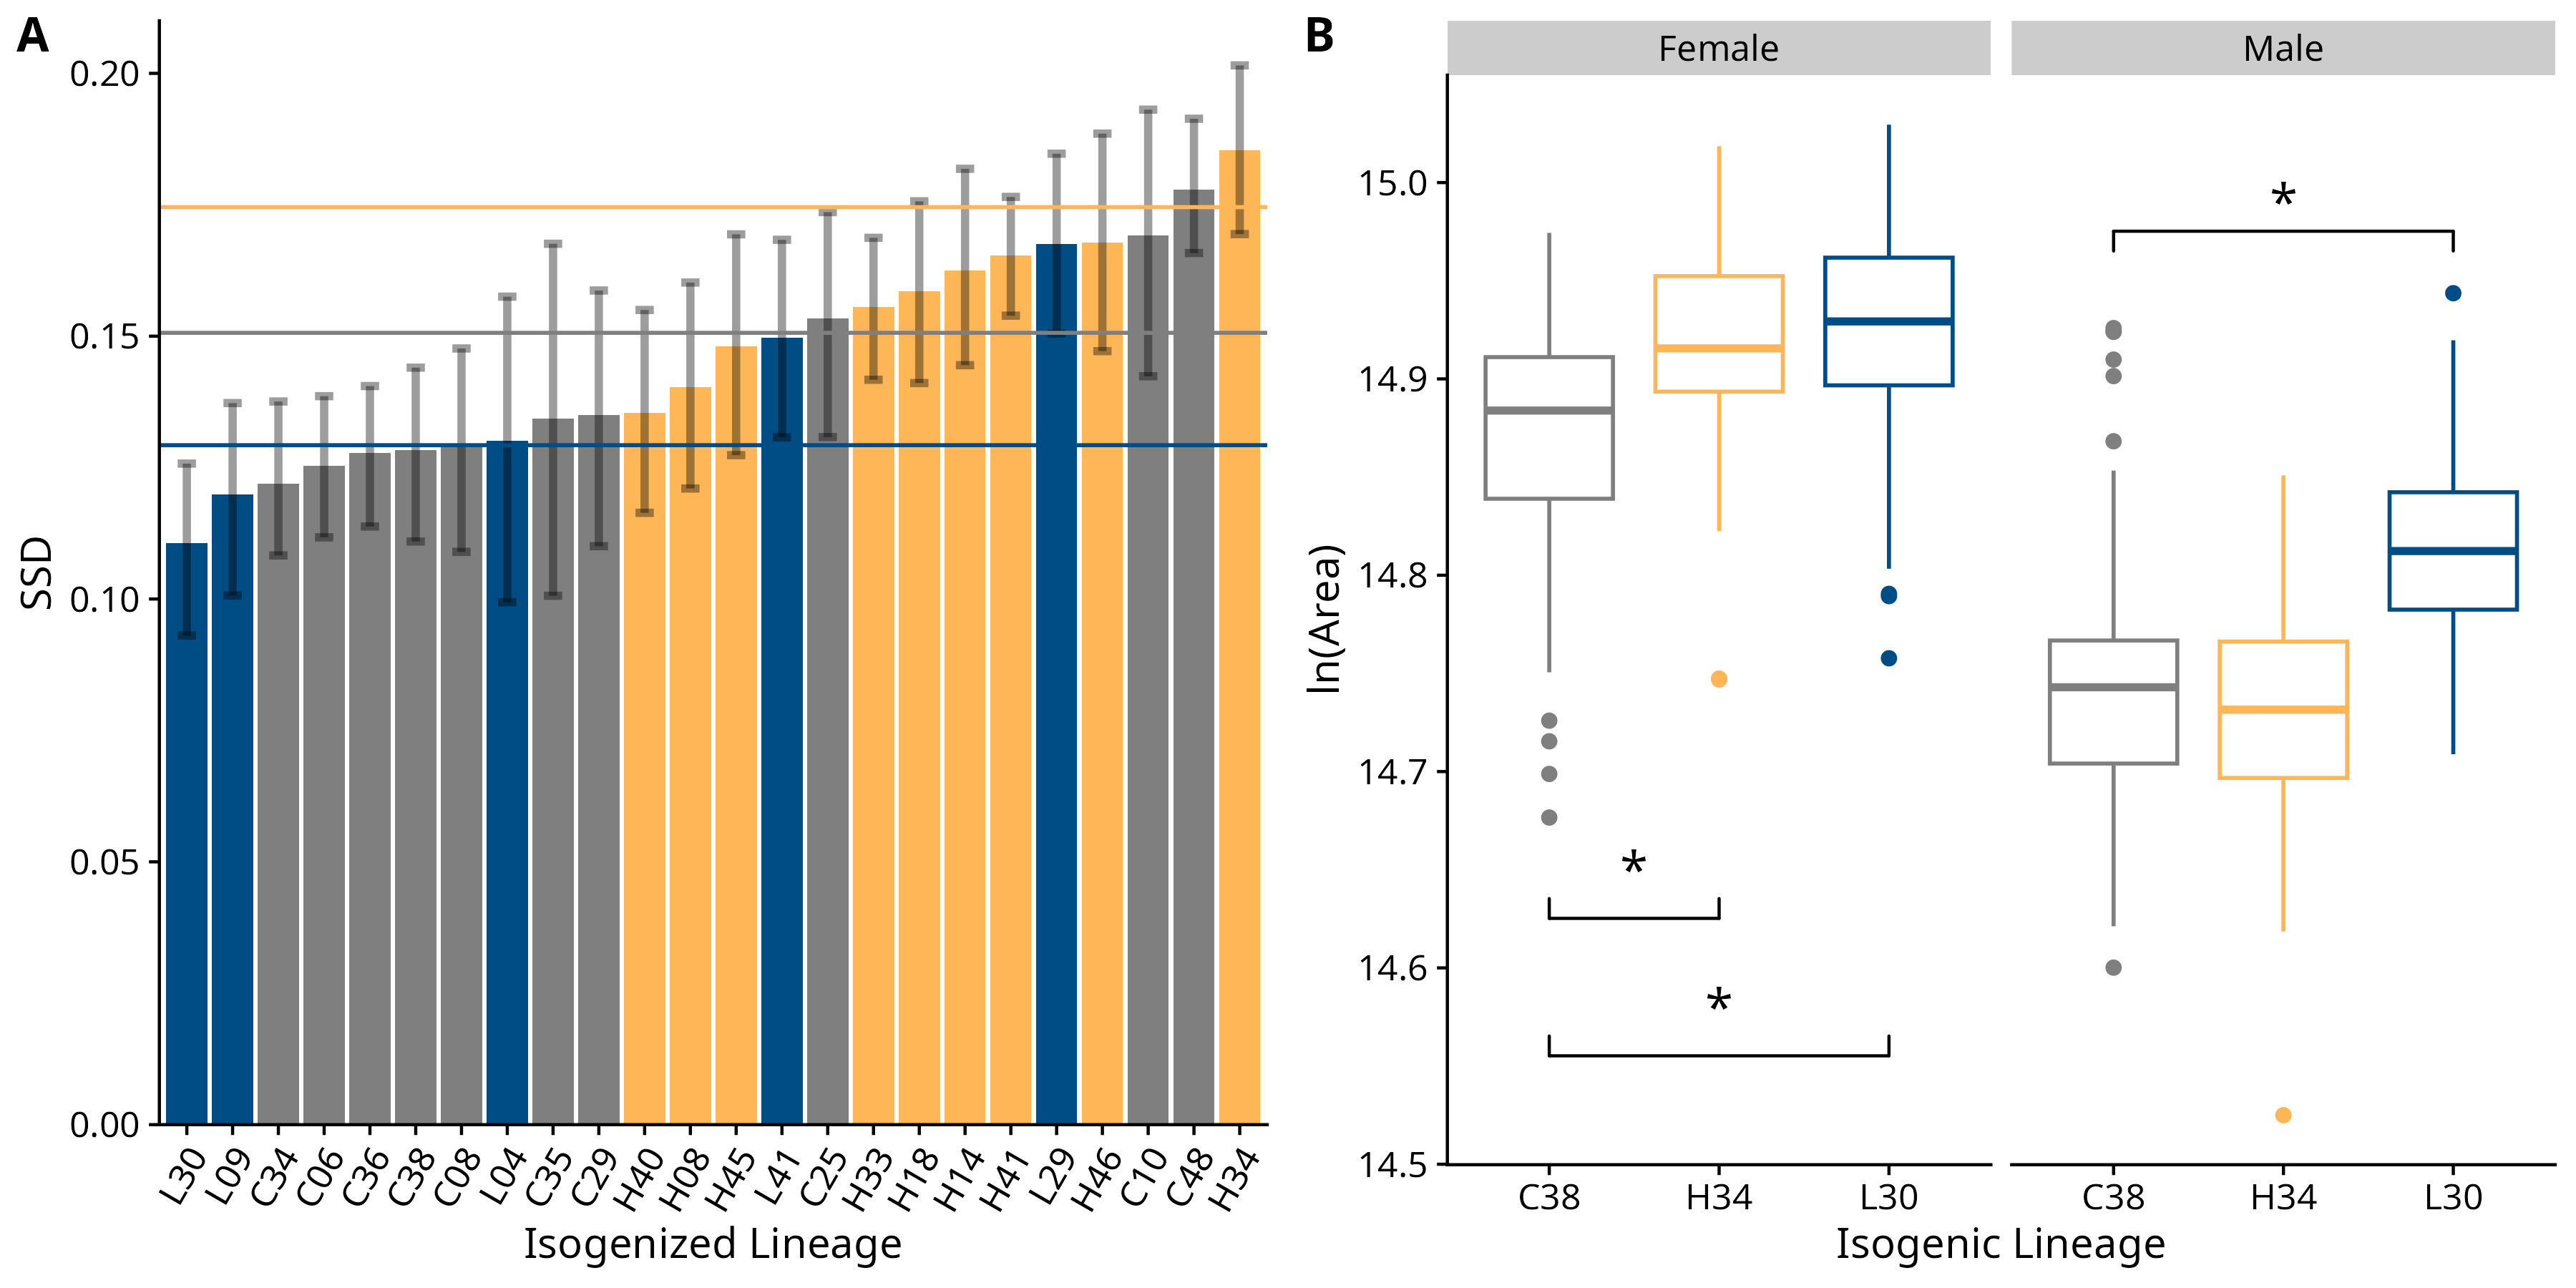
\includegraphics[alt = "SSD of isogenized lineages shows H34 and L30 have most extreme SSDs.", width=1\linewidth]{combinedSSD.png}
    \caption{Isogenized lineages H34 and L30 have more extreme SSD than their source populations (A) SSD of isogenized lineages. Horizontal lines represent (in descending order) the means of the total population of final generation of the selection study the high SSD lineage, the control lineage, and the low SSD lineage. (B) Sex specific body size of isogenized lineages selected for further study. Both H34 females, and both sexes of L30 being larger than their C38 counterparts reflects the differences in body size observed in the original selection experiment.}
    \label{fig:isogenizedSSD}
\end{figure}

SSD did not differ across treatments (ANOVA: F\(_{2,21}\) = 2.96, $P$ = 0.074). Lineages H34 and L30 had the most extreme SSD values. Among the controls, C38 was originally identified as having sex-specific sizes closest to its source population. Body size differences between these lineages mirrored the original selection response (see Chapter 2). Female body size  differed across lineages (ANOVA: F\(_{2,251}\) = 24.94, $P$ < 0.001). Both H34 (difference = +0.048, $P$ < 0.001) and L30 females (difference = +0.055, $P$ < 0.001) were larger than C38 females, but did not differ from each other ($P$ = 0.727). Male body size also differed across lineages (ANOVA: F\(_{2,269}\) = 49.75, $P$ < 0.001). Among males, L30 was larger than both C38 (difference = +0.072, $P$ < 0.001) and H34 (difference = +0.081, $P$ < 0.001), while H34 and C38 did not differ ($P$ = 0.509) (\textbf{Figure 1B}). Thus, the isogenized lineages retained the sex-specific body sizes of the source populations, confirming their utility for downstream characterization. From here on H34, C38, and L30 will be referred to as HL, CL, and LL.

\subsection{Causative Traits}

\subsubsection{Female MVW Increased for Selected Lineages}

\begin{figure}
    \centering
    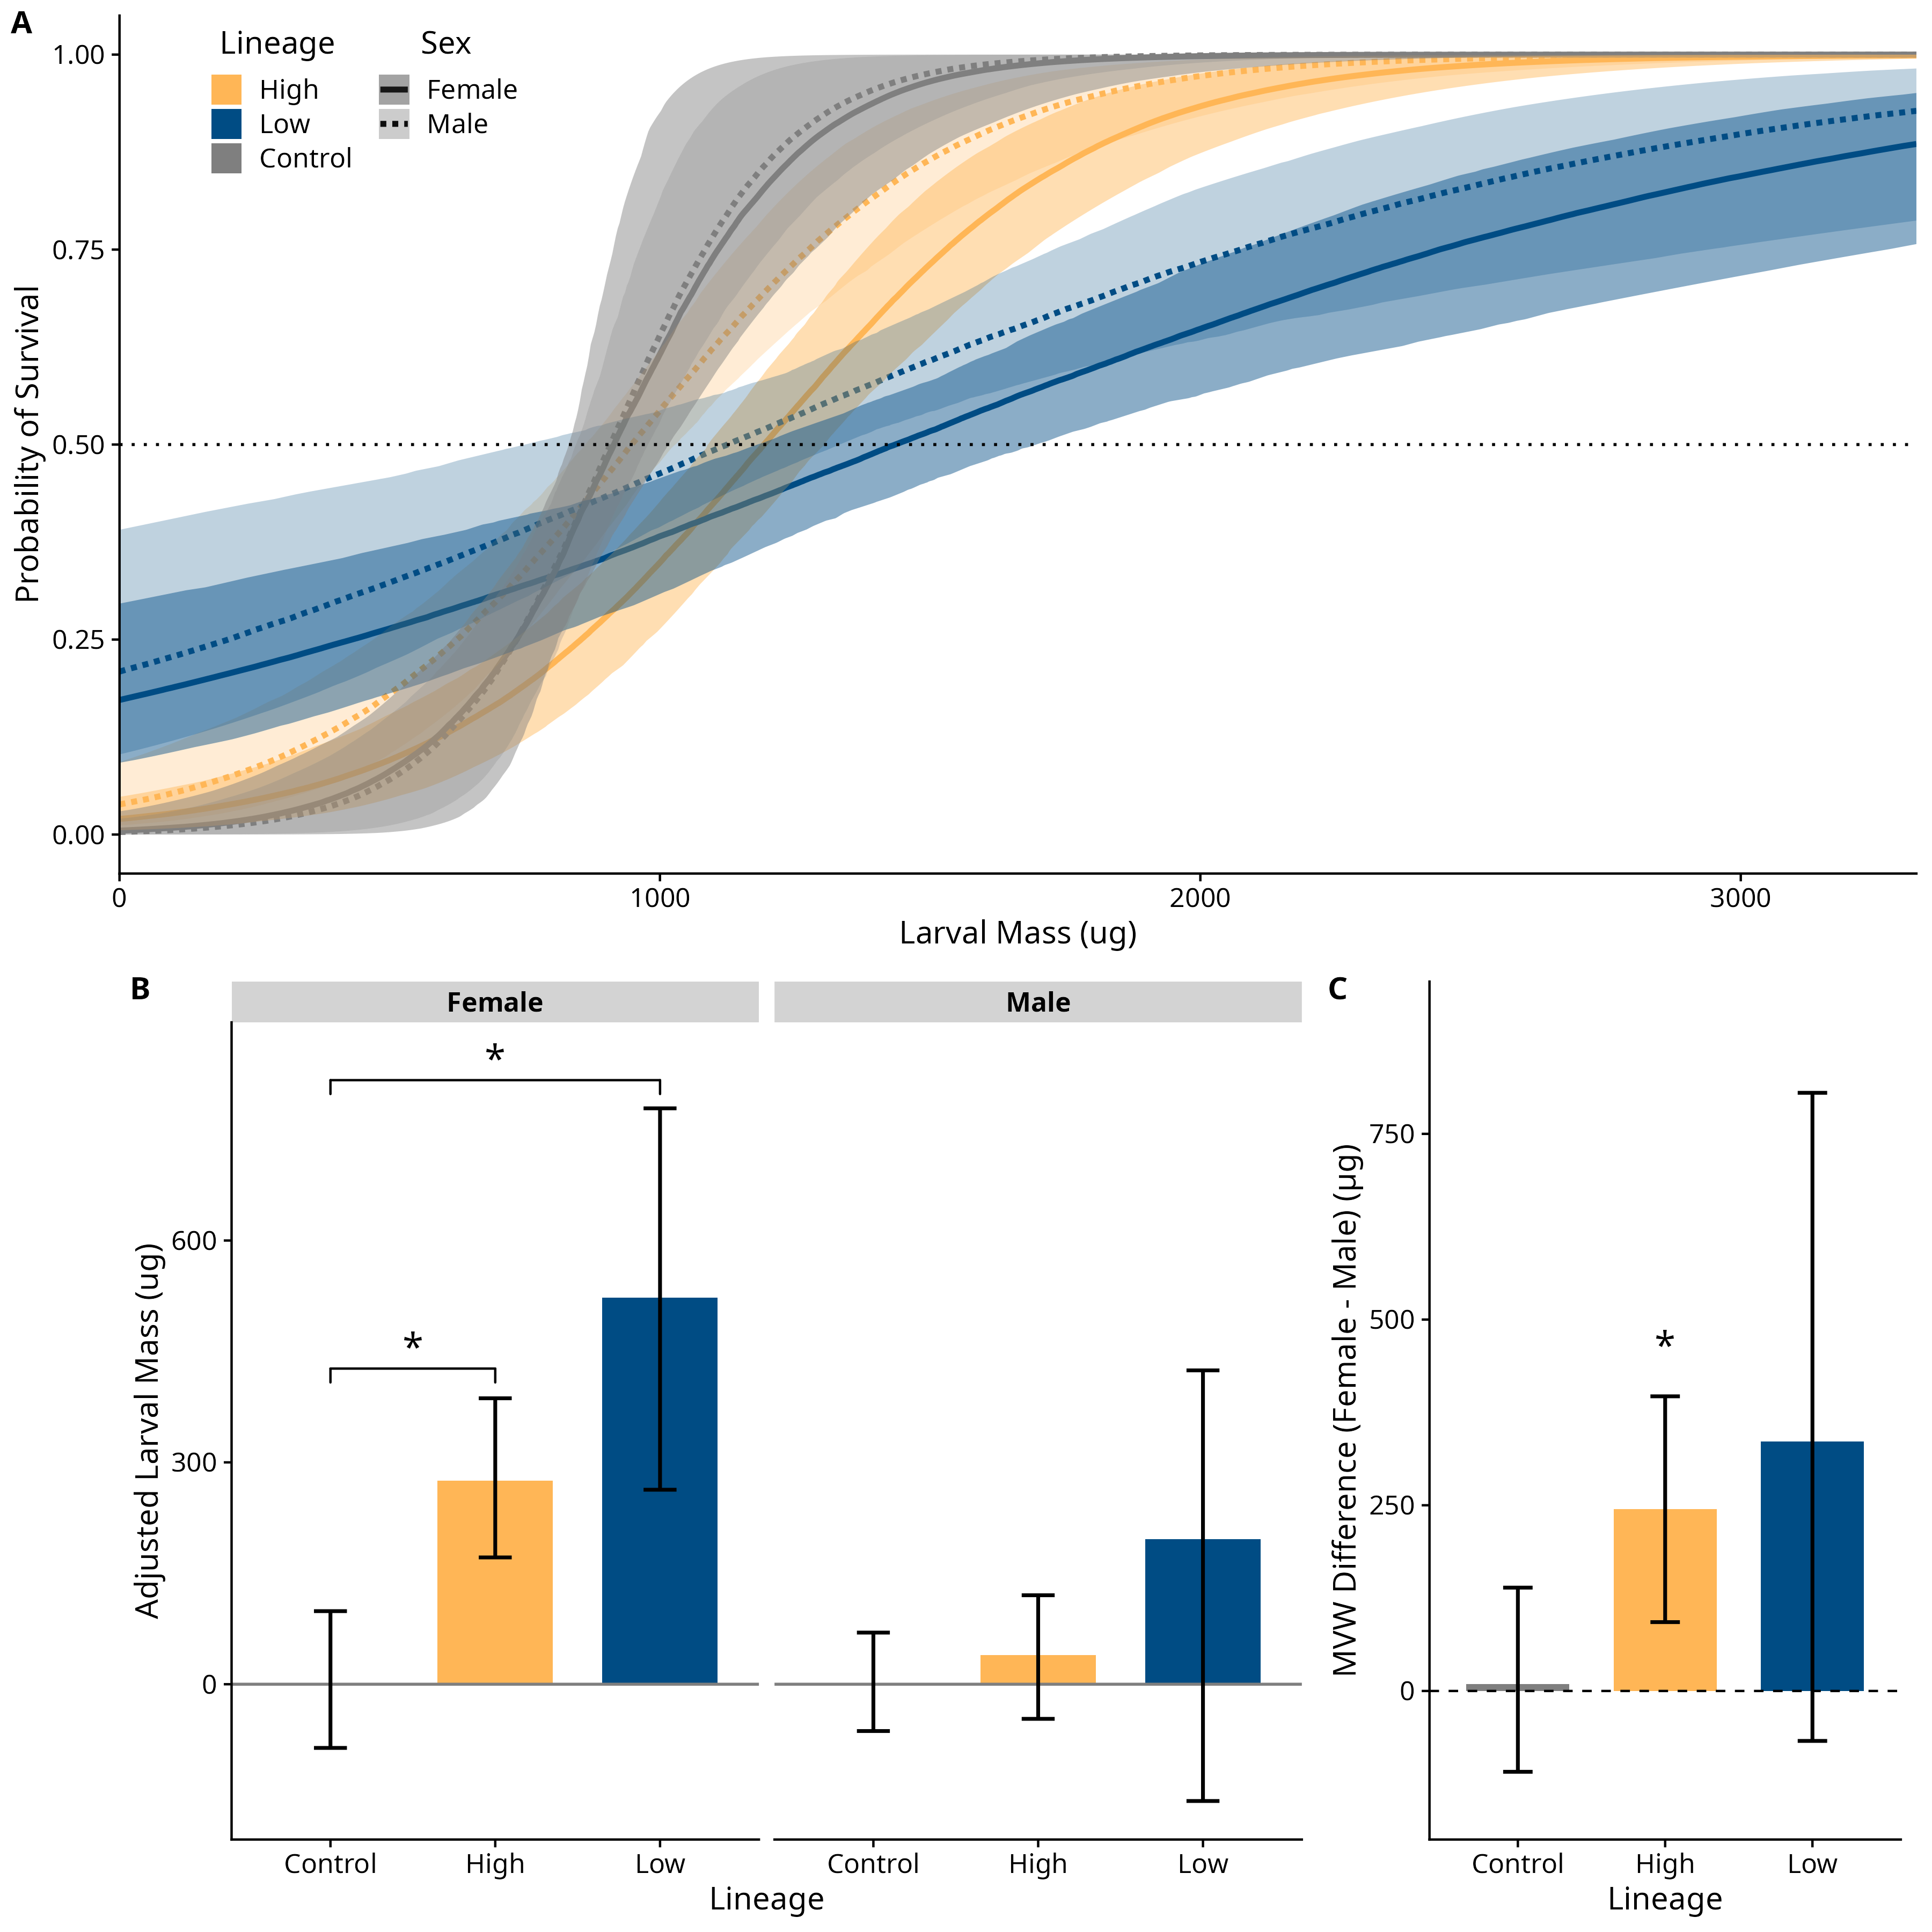
\includegraphics[alt = "Minimal viable weight across lineages and sexes.", width=1\linewidth]{MVW_combined_full.png}
    \caption{Minimal viable weight (MVW) across lineages and sexes. Asterisks denote significant sex differences within each lineage, determined if Bonferroni adjusted confidence interval of difference between groups did not contain zero. (A) Probability of successful eclosion as a function of larval mass, derived from logistic regression models fit to 1000 bootstrap resamples. Shaded ribbons represent 95\% credibility intervals. The dotted horizontal line marks 50\% survival probability; MVW is defined as the larval mass at which each curve crosses this threshold. (B) Adjusted sex sex-specific MVW estimates with whiskers reflecting the 95\% credibility intervals. (C) Differences in MVW between the sexes within lineages.}
    \label{fig:MVWadjusted}
\end{figure}

For MVW, the HL showed a significant sex difference with females requiring larger mass to reach eclosion than males (H: 245 µg, 95\% CI: 39-447) (\textbf{Figure 2C}). Both selected lines had significantly higher female MVW than Controls (HL-CL: 275 µg, 95\% CI: 74-460; LL-CL: 522 µg, 95\% CI: 118-902) (\textbf{Figure 2B}). No other pairwise comparisons of MVW were significant. Notably, the LL sex specific difference in MVW (336 µg) was not significant due to wide confidence intervals, particularly those of the LL male MVW estimates (\textbf{Figure 2B and 2C}).

\subsubsection{Females from Selected Lineages Matured Faster}

\begin{figure}[ht]
    \centering
    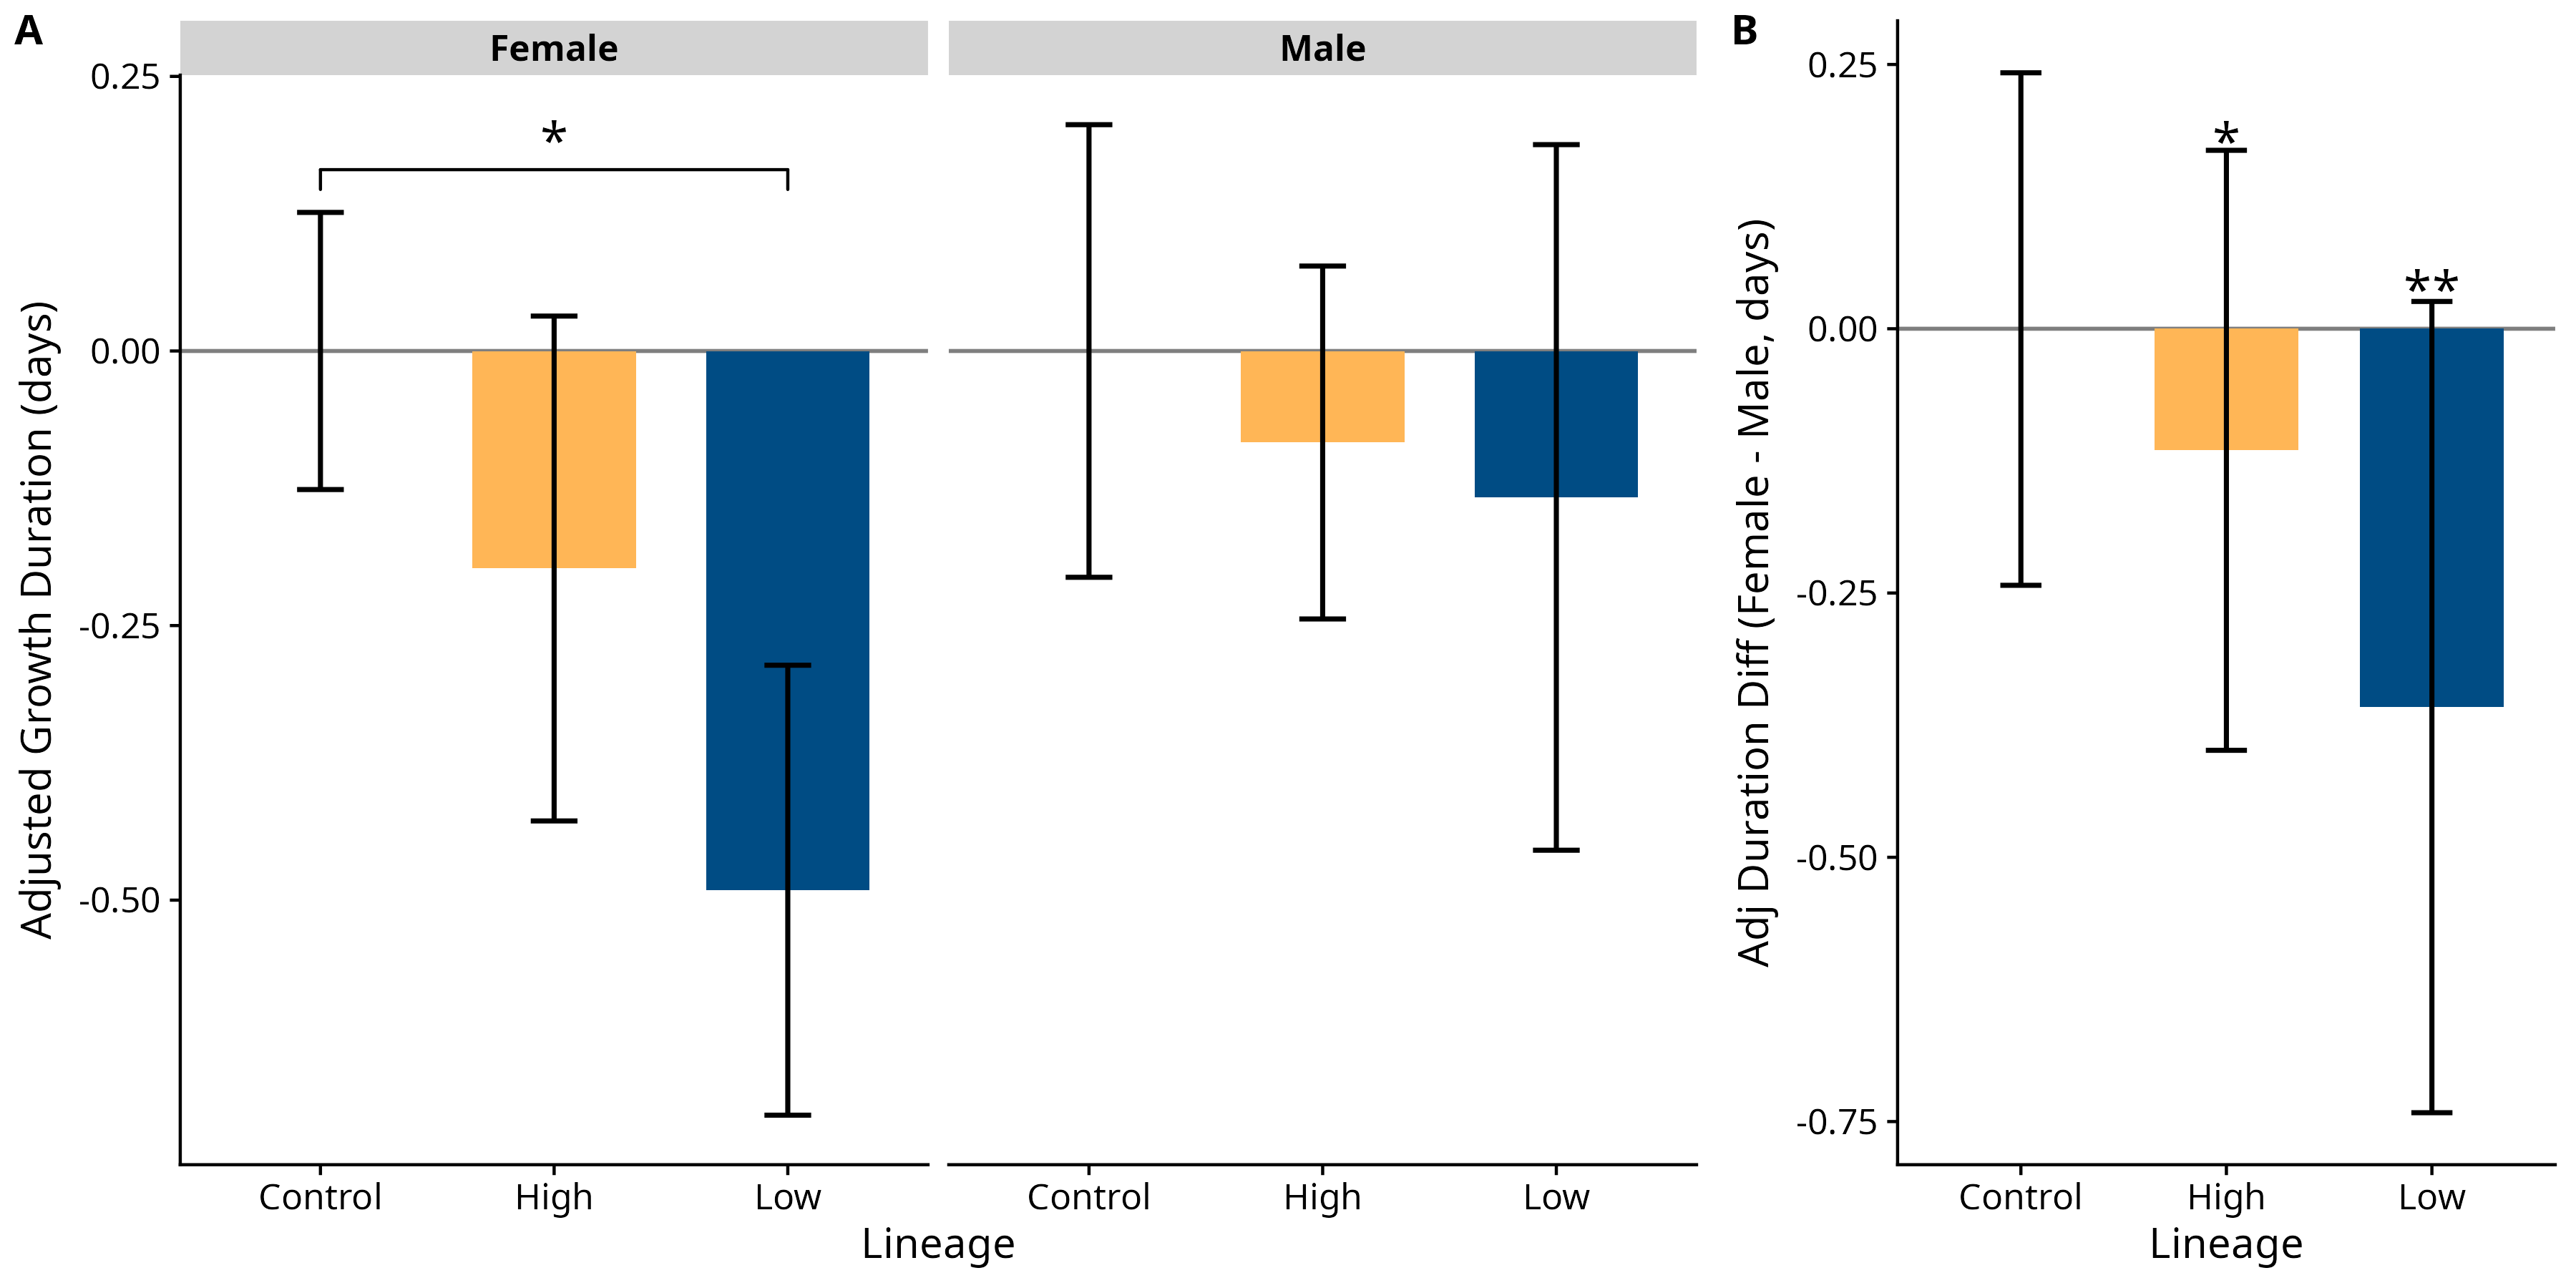
\includegraphics[alt = "Adjusted durations of growth.", width=1\linewidth]{durationCombinedAdj.png}
    \caption{Adjusted duration of growth. (A) By lineage and sex. LF vs CF are significantly different from one another (ANOVA: F\(_{2,94}\) = 8.63, $P$ < 0.001). Male developmental timing did not differ across lineages ($P$ = 0.71). (B) Difference between the duration of growth of the sexes. Welch t-testing found that CL sexes did not differ significantly ($P$ = 0.09), while the selected lineages had significant differences in developmental time between the sexes (HL $P$ = 0.02, LL $P$ < 0.01) with females had a shorter growth duration than their male counterparts.}
    \label{fig:durationCombined}
\end{figure}

Developmental time did not differ among males across lineages (ANOVA: F\(_{2,84}\) = 0.34, $P$ = 0.71; all pairwise comparisons $P$ > 0.70). In contrast, female developmental time differed significantly across lineages (ANOVA: F\(_{2,94}\) = 8.63, $P$ < 0.001), with LL females emerging approximately 12 hours earlier than Control females (Tukey HSD: $P$ < 0.001). HL females were intermediate and did not differ significantly from either Control ($P$ = 0.26) or LL ($P$ = 0.08) females.

Sex differences in developmental time were lineage-dependent. CL sexes did not differ (t = -1.71, $P$ = 0.09), but significant differences emerged in both selected lineages: HL females developed approximately seven hours faster than males ($P$ = 0.023), and LL females developed more than 13 hours faster than males ($P$ = 0.004). Thus, female duration of development took longer in the selected lineages, particularly in the ll.

\subsubsection{Females from Selected Lineages Grew at the Fastest Rates}

Growth rates were compared between sexes within each lineage and between lineages for the same sex using bootstrap resampling with Bonferroni correction for seven comparisons (\(\alpha\) = 0.05/7). All within lineage differences were statistically significant, females had significantly higher growth rates than males in all three lines (CL: difference = 0.025, 95\% CI: 0.013-0.039; HL: 0.038, 95\% CI: 0.023--0.053; LL: 0.040, 95\% CI: 0.020-0.061) (\textbf{Figure 4B}). Across lineages, females from both selected lines had significantly higher growth rates than CL females (HL vs. CL: 0.015, 95\% CI: 0.001-0.029; LL vs. CL: 0.030, 95\% CI: 0.015-0.045) (\textbf{Figure 4A}). In contrast, male growth rates did not differ significantly between any lineages. Thus, selection on SSD increased female growth rate while leaving male growth rate unaffected.

%REPLACE WITH UPDATED
\begin{figure}[t!]
    \centering
    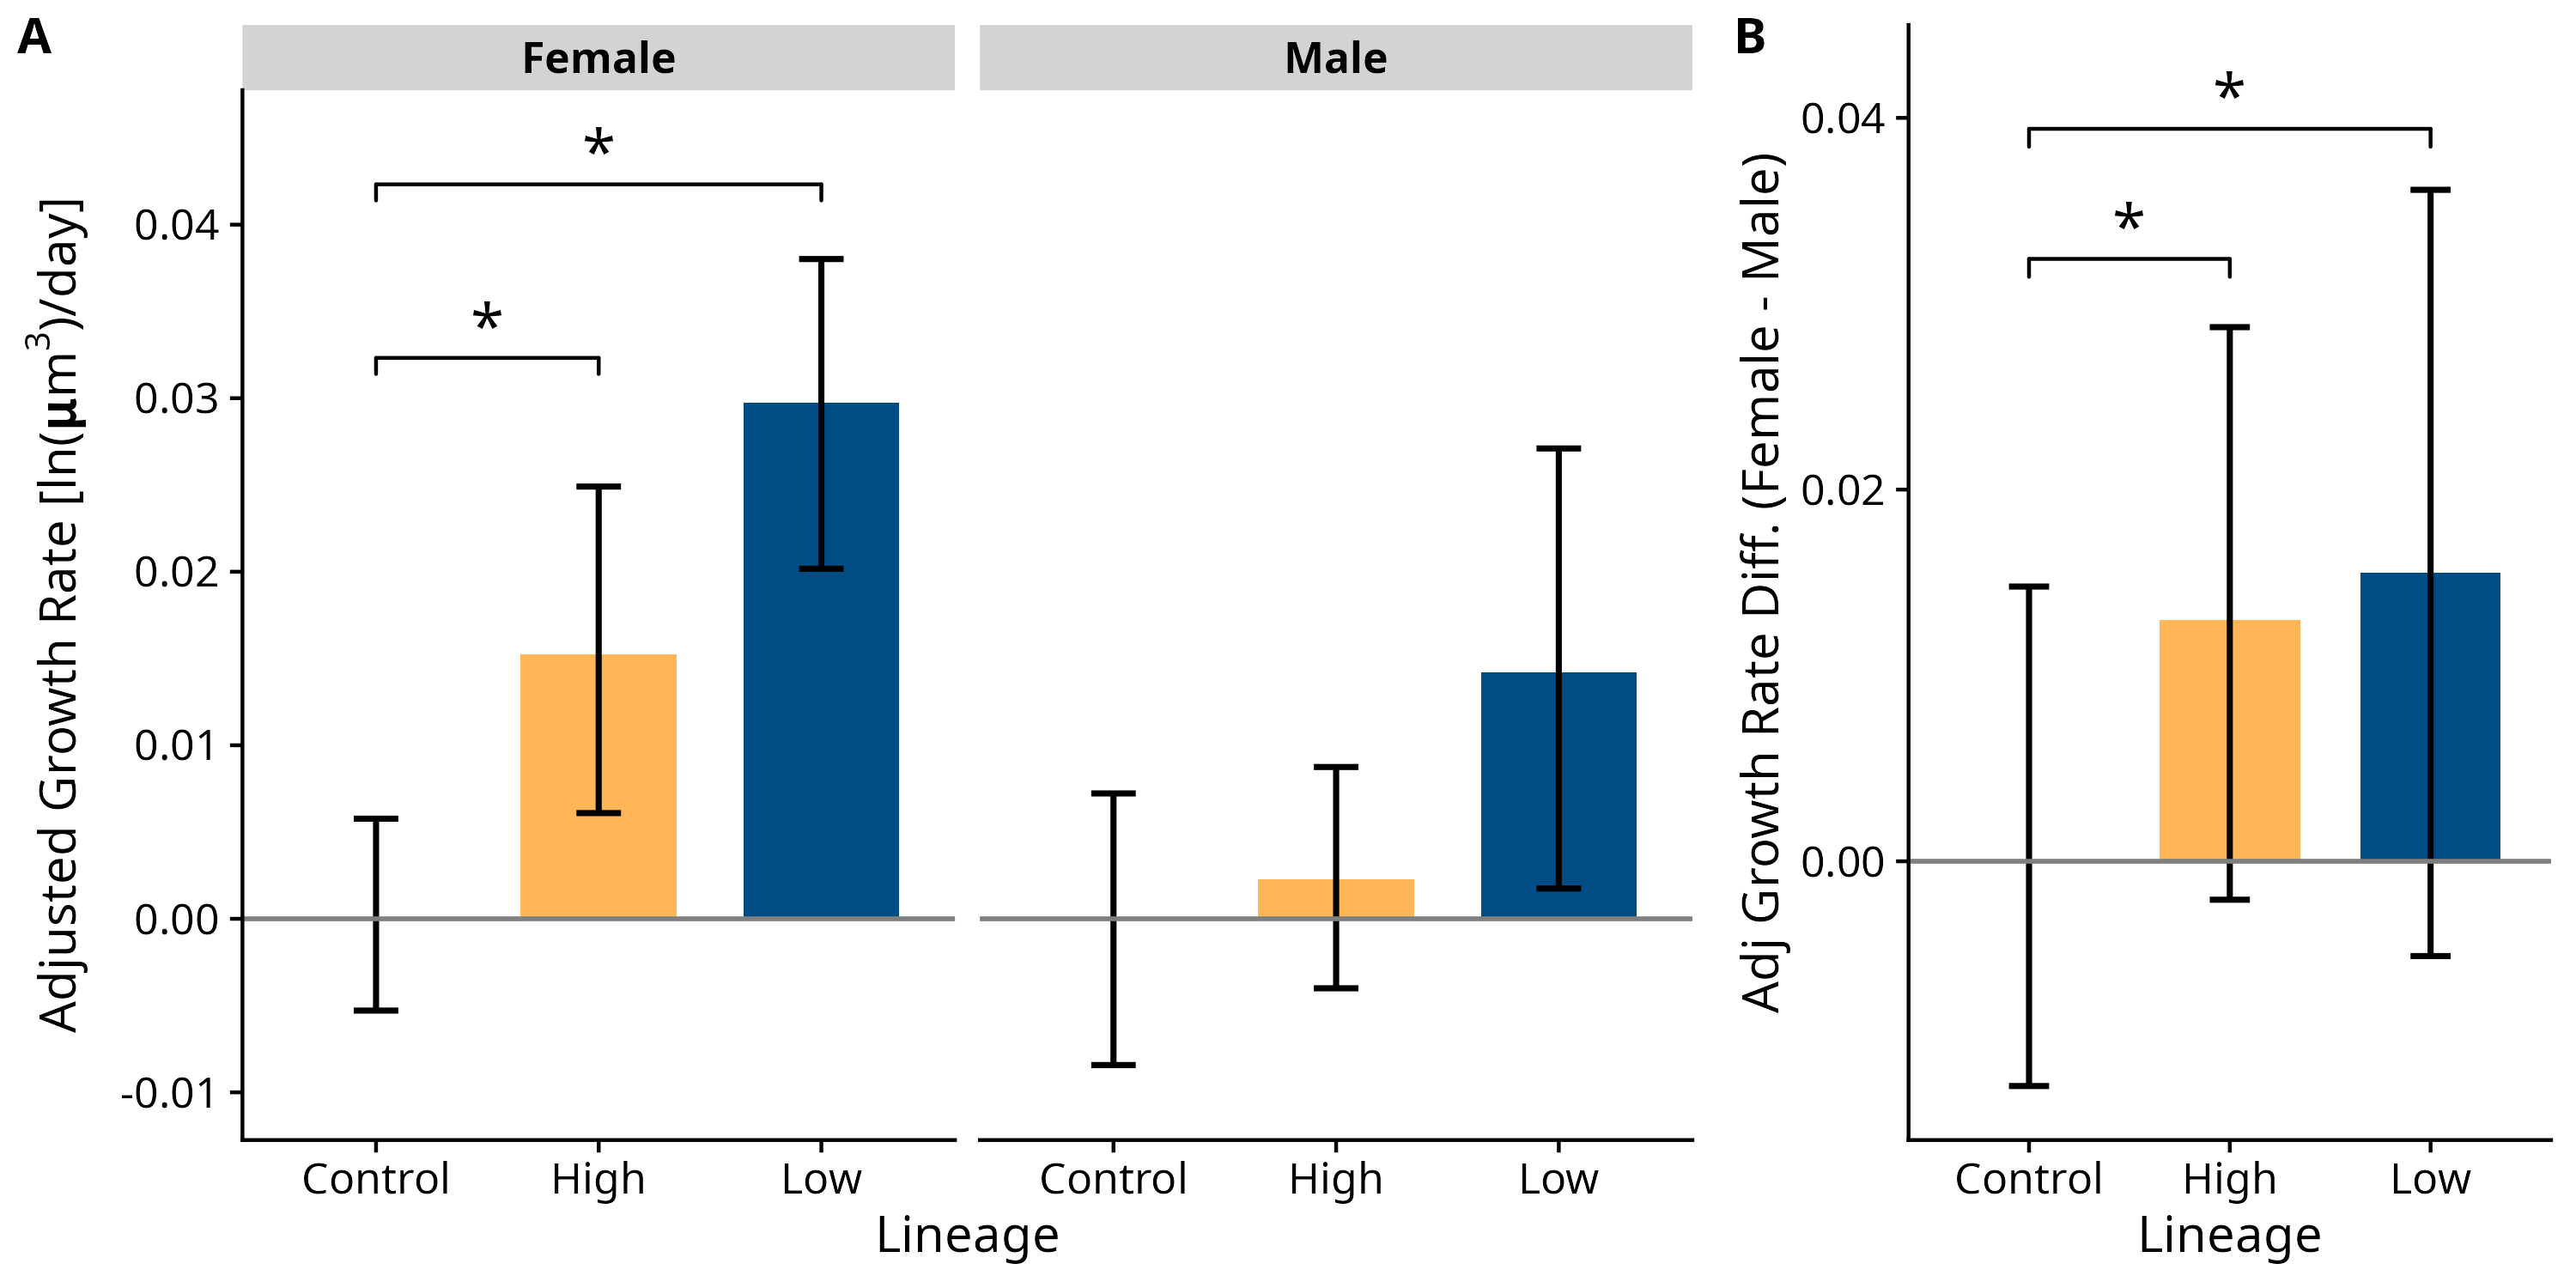
\includegraphics[alt = "Adjusted estimated growth rates across lineages.", width=1\linewidth]{growth_rate_combined_adj.png}
    \caption{Adjusted estimated growth rates across lineages. Asterisks denote significant sex differences within each lineage, determined if Bonferroni adjusted confidence interval of difference between groups did not contain zero. (A) Growth rates faceted by sex. Females of selected lineages differed significantly from controls, while males of all lineages did not. (B) Within lineage comparisons. The sexes of each lineage differed significantly, with females having a faster growth rate in each lineage.}
    \label{fig:growthratecombined}
\end{figure}

\subsection{Consequential Traits}

\subsubsection{Selected Lineages Had Low Fecundity}

Fecundity differed significantly among lineages (ANOVA: \(F_{2,20}\) = 12.79, $P$ < 0.001). Control females laid the most eggs (102.9 ± 9.4 eggs/24h), followed by Low line females (55.3 ± 7.5 eggs) and High line females (35.9 ± 4.5 eggs). Pairwise comparisons showed that both High and Low lines produced significantly fewer eggs than Controls (High: -67.0 eggs, $P$ < 0.001; Low: -47.6 eggs, $P$ = 0.005), while High and Low lines did not differ from each other ($P$ = 0.357). These results were confirmed by a linear mixed model with block as a random intercept (line effect: \(F_{2,19}\) = 12.80, $P$ < 0.001), and residuals met normality assumptions (Shapiro-Wilk: $P$ = 0.69). Thus, changing SSD reduced female fecundity.

\subsubsection{Low Egg-to-Adult Viability Among Selected Lineages}

Egg-to-adult viability did not differ significantly between sexes within the Control lineage (\(X^2\) = 1.57, df = 1, $P$ = 0.21) or the High lineage (\(X^2\) = 0.90, df = 1, $P$ = 0.34). The Low lineage showed a marginal trend toward higher female than male viability (\(X^2\) = 3.41, $P$ = 0.065).

In contrast, viability differed significantly across lineages for both sexes. Female viability varied among lineages (\(X^2\) = 8.76, df = 2, $P$ = 0.013), as did male viability (\(X^2\) = 22.45, df = 2, $P$ < 0.001). Total viability differed significantly across all lineages (\(X^2\) = 39.11, df = 2, $P$ < 0.001). However when comparing surviving females and surviving males between the selected lineages, they did not differ significantly (\(X^2\) = 0.63, df = 1, p-value = 0.43). These results indicate that selection on SSD reduced viability consistently across lineages and sexes. 

\subsubsection{Life Expectancy Diverged With SSD}

\begin{figure}
        \centering
        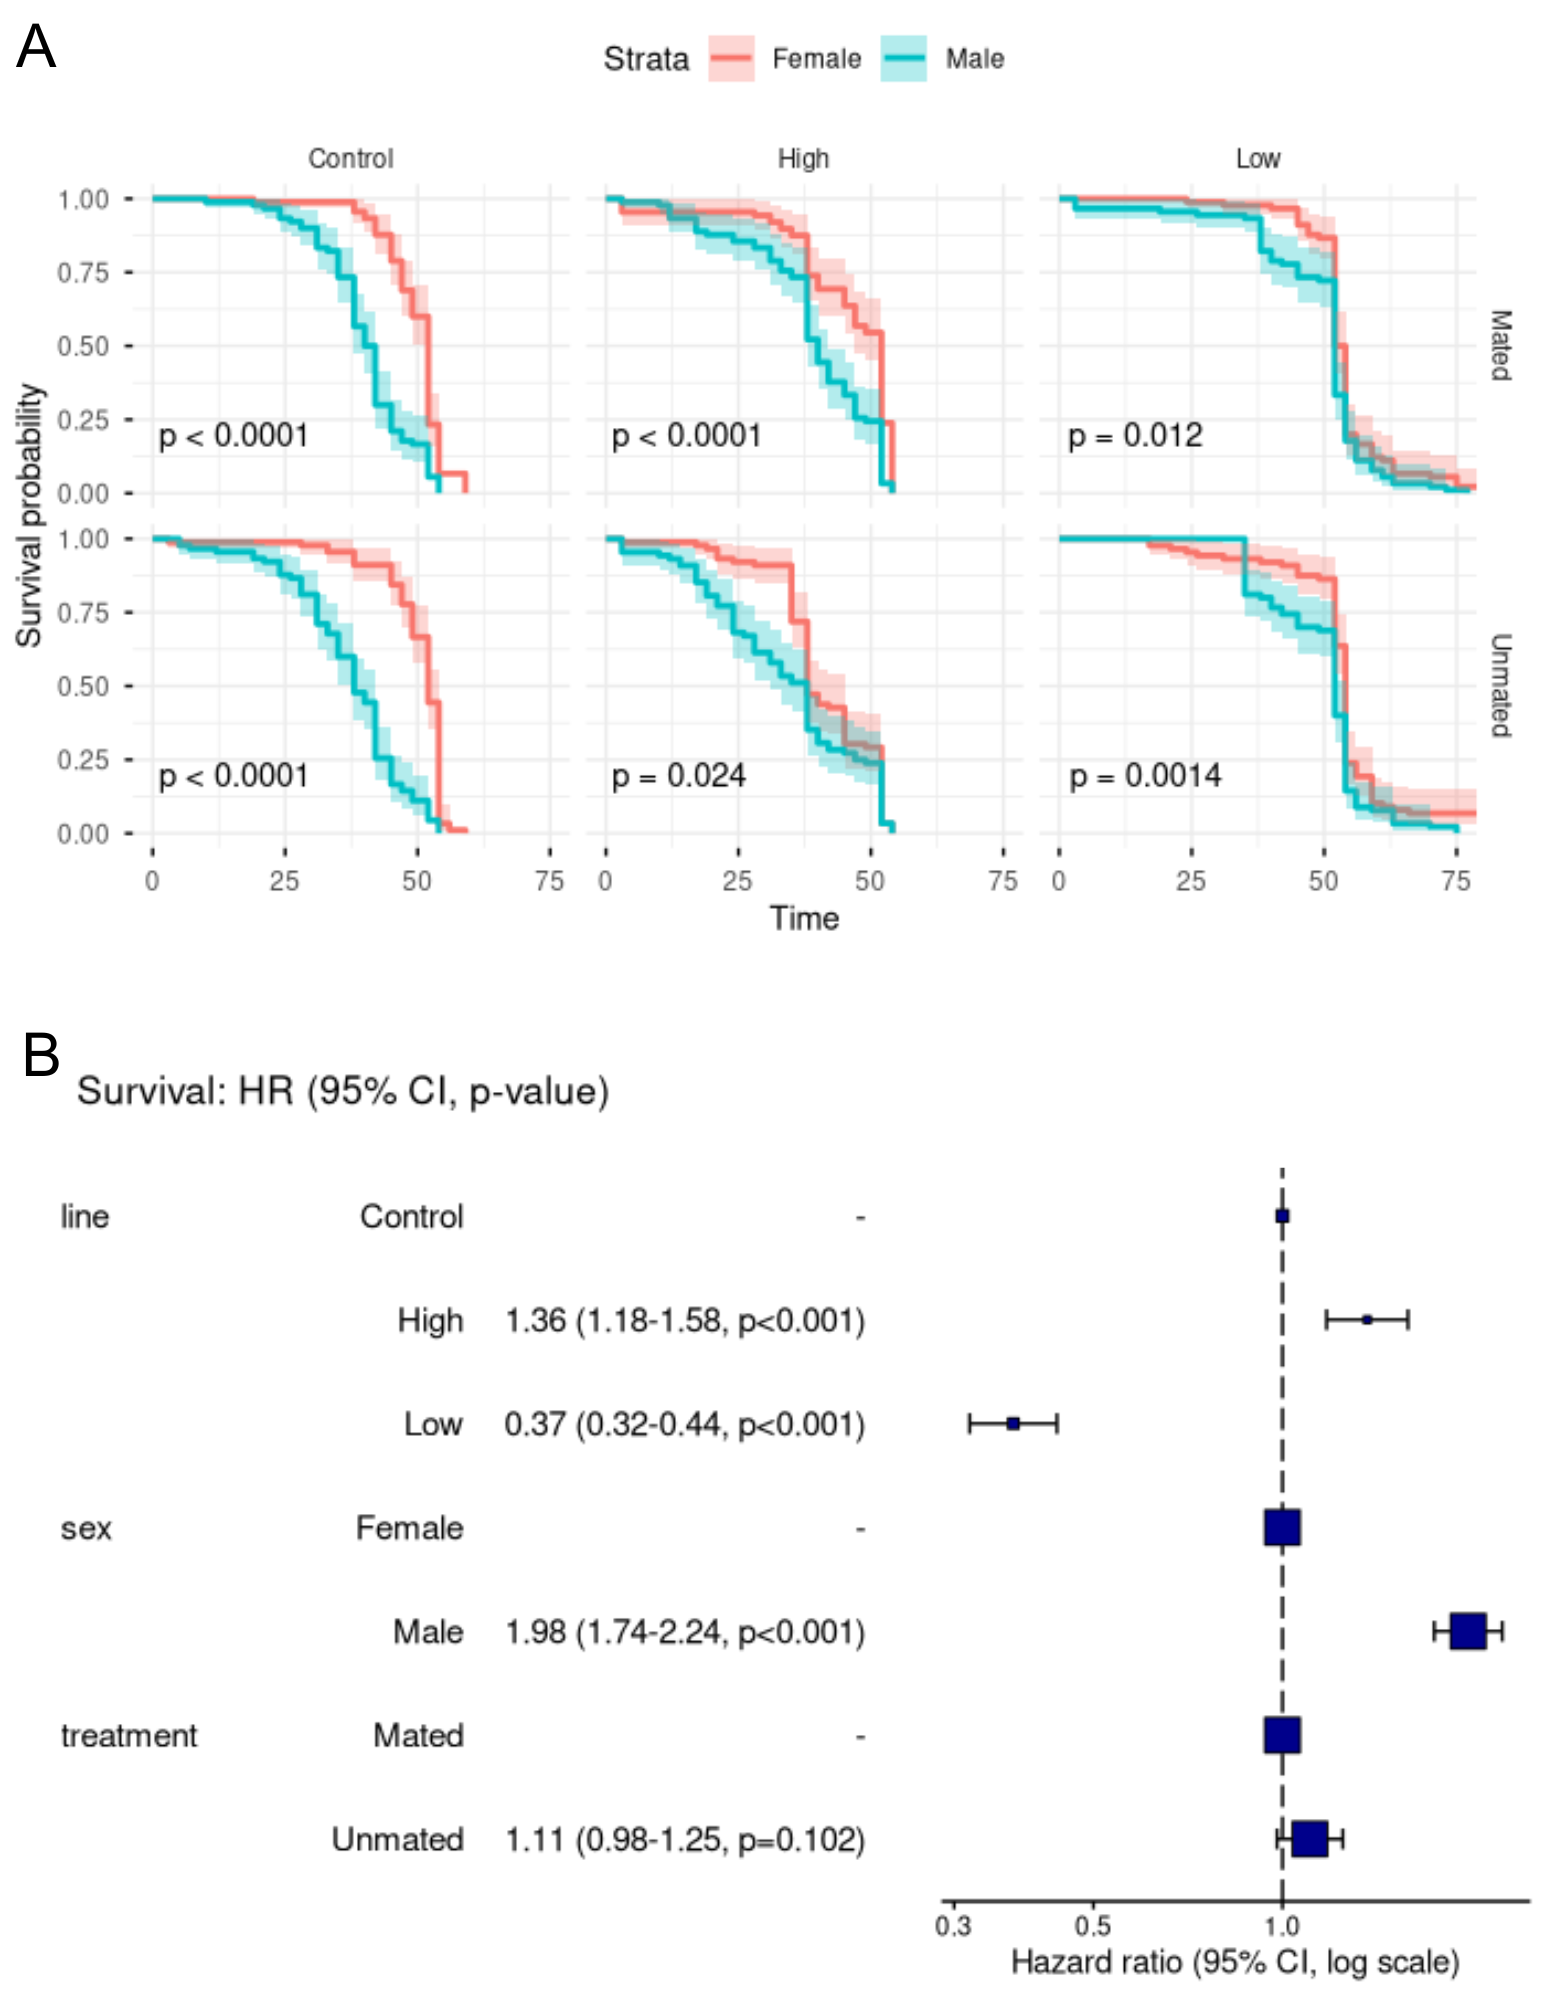
\includegraphics[alt = "Survival analysis.", width=0.75\linewidth]{SurvivalFig.png}
        \caption{Survival analysis of aging across lineages and treatments. (A) Kaplan-Meier survival curves showing the proportion of flies surviving over time, faceted by lineage (Control, High, Low) and mating treatment (Mated vs. Unmated). Curves are stratified by sex (Female: red; Male: blue). Shaded bands represent 95\% confidence intervals. P-values indicate significant differences between sexes within each facet, as determined by log-rank tests. (B) Risk table showing the number of individuals remaining at risk at each time point, stratified by the same experimental groups. A hazard ratio (HR) > 1 means that the group is more likely to die compared to the controls.}
        \label{fig:survival}
\end{figure}

While mating treatment did not effect longevity ($P$ = 0.102), lineage and sex were both had significant effects on longevity. When comparing rates of senescence of the selected lineages to controls, HL individuals died younger (HR = 1.36, $P$ < 0.001), and LL individuals lived much longer (HR = 0.37, $P$ < 0.001) with a small number of individuals surviving past 75 days of adulthood. 

\subsubsection{Wing-Body Scaling}

\begin{figure}
    \centering
    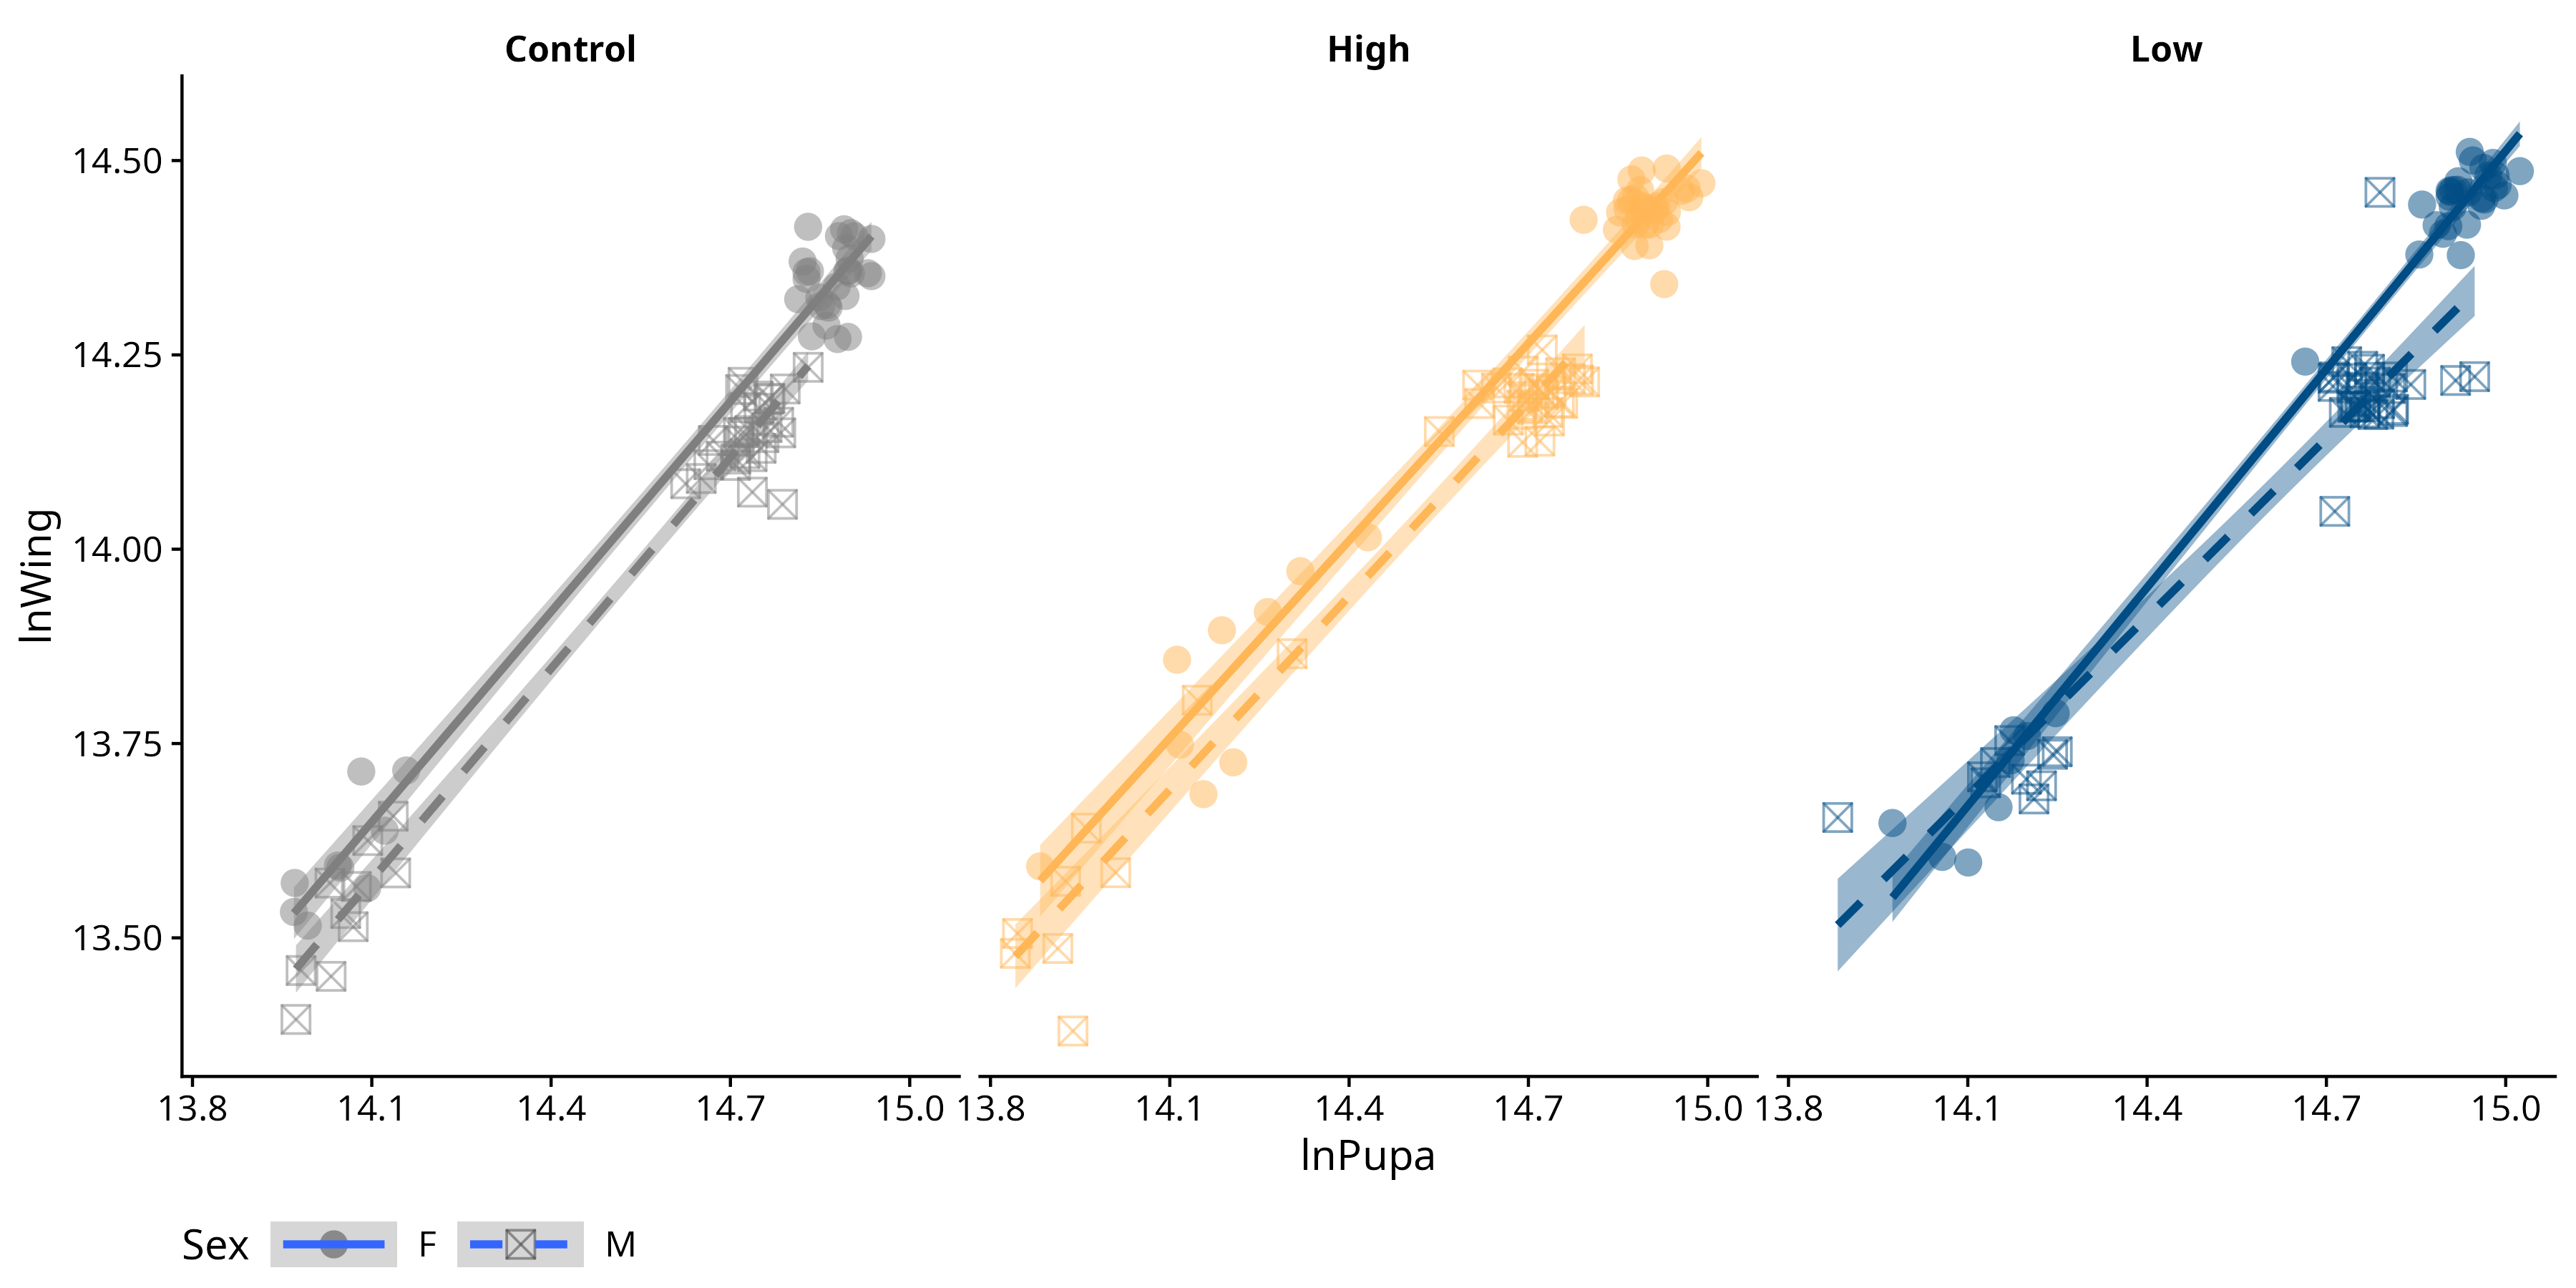
\includegraphics[alt = "Sex specific scaling of the wing against body size.", width=1\linewidth]{facet_ssp.png}
    \caption{Sex specific scaling of the wing against body size faceted by lineage.}
    \label{fig:scaling}
\end{figure}

Differences in these slopes between sexes and across lineages indicate variation in wing-body scaling. Slopes differ between lineages ($P$ = 0.035). Slopes differ between sexes ($P$ = 0.007). The effect of lineage on sex differences in slopes is significant ($P$ = 0.002). The strongest effect is in the LL, where males and females have significantly different slopes ($P$ = 0.001), while in other treatments, male and female slopes are parallel.

\section{Discussion}

The goal of characterizing causative and consequential traits of these isogenic lineages was to elucidate the causes and limitations on the evolution of SSD. This lineages present a unique opportunity to examine what direct selection on SSD impacts developmentally, which provides insight into the developmental factors regulating SSD and life-history related constraints the evolution of SSD. 

\subsection{Causative Traits: No Singular Trait Underlying Change in SSD}

\subsubsection{MVW Can Explain Size Increases but Cannot Explain LL Changes}

If MVW was the underlying cause for the observed differences in SSD, HL females and LL males would have had an increased MVW. Relative to the controls, the HL had larger females and males the same size. Likewise MVW increased for females and stayed the same relative to controls. While that appears to be a clean explanation for the observed difference for the HL, this is not the case for the LL which had increased MVW for both sexes. A possible explanation for this is that selecting on reduced SSD selected for an increase in male MVW, and there is pleiotropic effect increasing female size as well. The increase in MVW does however align with the groups that experienced increased in body size; HL females, LL females, and LL males. This suggests that an increase in MVW does correspond to an increase in body size, and could explain the increase in SSD in the HL but MVW does appear to have any involvement in reducing SSD for the LL.

\subsubsection{Duration of Development Cannot Explain HL Changes}

Testa et al. (2013) found that the duration of growth was not significantly different for the sexes, and this is also the case for my control lineage ($P$ = 0.09). However, Testa et al. (2013) found males had a slightly shorter growth duration, while for all my lineages females having the shorter growth duration, suggesting the direction might differ between populations. If the duration of development was the underlying cause for the observed difference in SSD, the HL would have a smaller gap between the growth durations of the sexes or the females having a longer duration than the males (that is female duration of development occurring over the same amount of time or longer than their male counterparts), and the LL would have a wider gap in the duration of developmental time. The LL did respond as expected in terms of duration of development, though LL male duration did not differ from the controls while LL female duration decreased by approximately 12 hours. The HL, however, did not respond as expected as neither sex's duration of development differed significantly from the controls. Thus, while changes in duration of development could explain the observed SSD in the LL, it does not explain the SSD of the HL.

\subsubsection{Growth Rate Cannot Explain LL Changes}

If growth rate was the underlying cause of the observed differences in SSD, for the HL the difference in growth rate between the sexes would increase relative to the controls and the LL difference in growth rate between the sexes would decrease relative to the controls. While the difference in the growth rate for the HL sizes did increase, with females developing at a faster rate and males having no significant difference relative to the controls, LL males also had no difference relative to the controls and LL females had the fastest growth rate of all. Thus, while growth rate might explain the observed difference in the HL, what is observed in the LL is antithetical to what I expected. 

\subsubsection{Opposing Causative Traits: A Comparison to Testa et al. (2013)}

While this study looked at a variety of traits that might underlie the observed differences in SSD, no singular trait stood out as the obvious cause. Testa et al. (2013) previously established that sex-specific differences in body size arise from differences in four developmental factors: critical size, growth rate, growth duration, and mass loss. Testa et al. (2013) suggested based on their experimental work that SSD was primarily driven by growth rate and critical size, but not the duration of growth (Testa et al., 2013; Shingleton \& Vea, 2023).

Both Testa et al. (2013) and I found the duration of growth did not differ significantly between the sexes, however they found that females eclosed later. For all three of the lineages I assayed, males eclosed later. Testa et al. (2013) also found that females had a larger critical mass, and while this is true for my selected lineages, it is not the case for the CL. However these results come from an isogenic Samarkand stock back-crossed with \textit{Ubi-GFP}, and so what they observed might only hold true for this particular lineage. As mentioned earlier, Testa et al. (2013), also found that growth duration was longer for females, but amongst all my lineages growth duration is shorter for females (\textbf{Figure 4}. This might be indicative of the growth durations of the Fenn Valley Winery colony, the initial population from which the selected lineages were derived, or the direction of growth duration being highly variable. Therefore, measuring complete growth profiles for the most extreme SSD DGRP lineages and the most extreme lineages present here might give insight into which developmental mechanisms regulate SSD in \textit{D. melanogaster}.

\subsection{Consequential Traits: Correlation Between SSD and Fitness Components}

\subsubsection{Fecundity Declined For Both Selected Lineages}

The relationship between body size and fecundity has long been of interest in \textit{Drosophila} research (Tantawy \& Vetukhiv, 1960; Reeve \& Fairbairn, 1998; Lefranc \& Bundgaard, 2000; Novoseltsev et al., 2003). In this study, fecundity was dramatically reduced in both selected lineages compared to Controls (CL: 103 eggs/day; LL: 55 eggs/day; HL: 36 eggs/day).

These results are striking because both selected lineages have larger females than Controls (\textbf{Chapter 2}), and smaller female body size is generally associated with reduced fecundity (Lefranc \& Bundgaard, 2000). The direction of the effect also runs counter to expectations from Reeve and Fairbairn (1998), who found that selecting for increased fecundity increased SSD. If SSD and fecundity are genetically correlated, one might predict that the HL (selected for increased SSD) would have higher fecundity than CL. Instead, HL females had the lowest fecundity of all three lineages.

Lefranc and Bundgaard (2000) examined fecundity as a function of sex-specific body size combinations and found that pairs of average-sized individuals produced the most offspring. They also reported that matings between large females and small males (a combination resembling the HL) produced more offspring than matings between large females and large males (resembling the LL). However, in my study, the HL produced 19 fewer eggs per day than the LL, the opposite of what their results would predict.

Several factors may explain these discrepancies. First, Lefranc and Bundgaard (2000) manipulated body size through nutrition, whereas my lineages differ genetically. Environmental and genetic variation in body size may have different effects on fecundity. Second, my HL and LL lineages differ not only in body size but also in other traits affected by selection on SSD, including developmental timing, viability, and longevity. These correlated responses may obscure any relationship between body size and fecundity. Third, the isogenization process itself may have altered fecundity independently of body size, as inbreeding depression is known to affect reproductive traits (Wade et al., 1996).

Taken together, these results suggest that selection on SSD imposes a substantial fecundity cost that is not simply explained by changes in body size alone. Both selected lineages show reduced fecundity relative to Controls, with the HL, despite being selected for increased SSD, showing the greatest reduction. This trade-off may reflect pleiotropic effects of the alleles underlying SSD divergence on reproductive physiology.

\subsubsection{Viability Reduced Similarly for Selected Lineages}

Inbreeding has been shown to increase the variance for viability in \textit{D. melanogaster}, so it is possible that the isogenization process itself could account for the differences observed between lineages (Wade et al., 1996). However, that both selected lineages did not differ significantly from one another in egg-to-adult viability for either sex suggests that selection on SSD, and potentially the change in SSD, caused this reduction in viability.

\subsubsection{Lifespan Benefits from Reduced SSD}

The selected populations diverged from the CL not only in SSD, but in life expectancy, with the HL having a reduced life expectancy (HR = 1.36, $P$ < 0.001) and the LL having a longer life expectancy (HR = 0.37, $P$ < 0.001) (\textbf{Figure 5B}). This suggests that reducing SSD increases lifespan and increasing SSD reduces it. I also observed that though sex specific life expectancy remained significant for the LL, male life expectancy was closer to female life expectancy in this lineage more than any other, suggesting the reduction in SSD might also reduce the gap in life expectancy. However it could also be that the LL evolved an increased life expectancy to mitigate the effects of there be no weight at which LL pupae will almost certainly reach adulthood (\textbf{Figure 2A}), which fits with the theory of antagonistic pleiotropy (Shingleton \& Weed, 2025). %alex mentioned something in jun 5 zoom about this to be looked up later

\subsubsection{Selected Lineages Have Negative Consequences}

It seems that selecting upon SSD caused both divergent lineages to experience a decrease in fecundity and egg-to-adult viability. While the HL had a reduced life expectancy and the LL had an increased life expectancy. Also while wing-body scaling of the sexes of the CL and HL run parallel to one another, LL male wing-body scaling intersected with that of LL females. It could be that while while some of the traits explored in this paper are labeled as consequential traits, that many of the unexpected outcomes observed are actually due to the minimum requirements of these traits to maintain the isogenic lineages. That is to say, a trait like fecundity is necessary to sustain an isogenic lineage. %MORE HERE

\subsection{Evolved SSD Was Not Retained in All Isogenized Lineages}

Though the DGRP was isogenized over 20 generations of full-sibling inbreeding (Mackay, 2018), my isogenized lineages only underwent 10 generations of full-sibling inbreeding. Crucially, my founding populations were already somewhat inbred as a consequence of the 15 generations of family selection described in Chapter 2.

Although these lineages are derived from populations selected for divergent SSD, many lineages did not survive the isogenization process, and among those that did, the evolved SSD was not retained in many. This is likely because isogenization itself imposes strong selection (Wade et al., 1996), favoring traits that enhance survival under inbreeding rather than preserving the specific SSD phenotype generated by the original selection regime. Consequently, only a subset of isogenized lineages retained SSD values representative of their source populations and were used for further characterization.

Despite the loss of SSD in many lineages, isogenization offers a critical advantage: it removes the genetic noise present in heterogeneous populations, allowing observed phenotypic differences to be attributed to specific genotypes (Mackay, 2018). The lineages that did retain SSD therefore provide a powerful tool for linking genotype to phenotype in subsequent analyses.

\subsection{Future Directions}

As mentioned earlier, both this work and the work of Testa et al. (2013) are based on isogenic stocks. While Testa et al.'s proposed developmental regulators of SSD are conceptually straight-forward as the accumulated sex specific differences in critical size, growth rate, growth duration, and mass loss, the comparison of their results to my own suggests that these traits are highly variable between isogenic lineages (as discussed earlier). I suggest sex specific profiles be characterized as described in Testa et al. (2013) and consequential characteristics be assayed for several isogenic lineages:

\begin{itemize}
    \item Replicate lineages from this study that retained ancestral SSD (such as C25, H46, and L09)
    \item Lineages derived from the Fenn Valley Winery stock (the ancestral stock of the selection experiment described in Chapter 2)
    \item \textit{Drosophila} Genetic Reference Panel (DGRP) lineages with the most extreme SSD
\end{itemize}

Characterizing the growth profiles of these lineages would provide insight into what patterns of growth consistently regulate SSD among \textit{D. melanogaster} populations. Running assays on the consequential traits suggested here those same lineages could also provide insight as to whether SSD affects these traits directly or if the observed differences are a consequence of inbreeding fixing an unrelated phenotype. 

Genotyping the most divergent lineages may also provide insight as to the genetic underpinnings of these lineages. As the DGRP lineages are already genotyped and the SSD of many of these lineages has already been characterized (Vea et al., 2026), the lineages with the most extreme SSD could be compared with the isogenic lineages generated here.

\section{Conclusion}

This chapter aimed to distinguish between traits that cause SSD divergence and traits that are consequential byproducts of altered SSD using isogenized lineages derived from a 15-generation selection experiment. No single causative trait explained the observed differences in SSD; instead, selected lineages differed from Controls in a suite of consequential traits, particularly affecting females--both selected lineages had higher female minimal viable weight and faster female development, while male traits remained largely unchanged. The consequential traits revealed striking trade-offs: both selected lineages showed dramatically reduced fecundity and viability compared to Controls, with the High line (increased SSD) consistently performing worst across all fitness components, while the Low line (reduced SSD) showed a more complex pattern of reduced early-life fitness but increased lifespan. Together, these results demonstrate that SSD is not an isolated trait but is embedded in a network of correlated characteristics with important fitness consequences. The isogenized lineages characterized here provide a valuable resource for future work on the genetic architecture underlying these trade-offs.

\clearpage
\chapter{Conclusion}

In the previous chapters, I have described my E\&R study carried out to improve our understanding of the developmental-genetic mechanisms underlying sexual size dimorphism (SSD). In this chapter, I will summarize each of the chapters, contextualize my research within this field, and propose future experiments as a consequence of my findings.

\section{Summary of Findings}

SSD is one of the most obvious forms of sexual dimorphism, yet the developmental-genetic mechanisms regulating SSD remain largely unknown. Females and males share the vast majority of their genetic material but have differing sex-specific size optima, and this sex-specific selection generates SSD. Body size in animals is regulated by four developmental factors; (1) size at birth, (2) growth rate, (3) growth duration, and (4) mass loss. Sex specific differences in these factors accumulate to generate adult SSD (Testa et al., 2013). Insulin-like/IGF signaling (IIS) is necessary for SSD, as knockdown of IIS results in the loss of SSD (Testa et al., 2013), therefore I hypothesized my selection regime would target loci involved in the canonical IIS pathway. Sex-specific plasticity (SSP) and SSD are tightly correlated, suggesting an overlap in their underlying mechanisms (Vea et al., 2023). Genome-wide association studies (GWAS) and evolve and resequence studies (E\&R) are complementary approaches for identifying candidate genes associated with polygenic traits (Turner et al., 2013), and my these leveraged both to elucidate the genetic mechanisms underlying SSD.

In Chapter 2, I described the "evolve" portion of my E\&R study. Over 15 generations of family selection, SSD diverged between the high SSD lineage (HL) and low SSD lineage (LL) relative to the control lineage (CL). Changes in SSD reflected divergent responses in male body size between selected lineages, with female body size having increased in both lineages. The sex-specific responses deviated from my expectations, as HL males and LL females both had pressure to reduce in body size but did not. Through the process of elimination, the most parsimonious explanation for these unexpected responses is intralocus sexual conflict.

In Chapter 3, I described the "resequence" portion of my E\&R study. Using an adapted chi-square test, I identified candidate loci that responded to selection on SSD. The chi-square tests on the divergent lineages intersected at five candidate genes after filtering for control lineage hits. When comparing my selected lineages hits intersected at 14 of the 110 candidate genes associated with SSD identified by Vea et al.'s (2026) GWAS on the Drosophila Genetic Reference Panel. Only one gene \textit{unc-13-4A} was identified as a candidate gene for both HL, LL, and the DGRP GWAS.

In Chapter 4, I used isogenized lineages derived from the final selected populations to characterize causitive (traits that likely \textit{produce} the observed differences in SSD) and consequential traits (traits that may be \textit{affected} by changes in SSD). The isogenized lineages C38, H34, and L30 (derived from CL, HL, and LL respectively) had SSD and sex-specific sizing similar to their source populations. Though I tested three causitive traits -- minimum viable weight, developmental timing, and growth rate -- no single trait explained the observed divergence in SSD. Characterization of the consequential traits revealed that selected lineage had both reduced fecundity and reduced egg-to-adult viability, but diverged in regards to lifespan, with the HL having a decreased lifespan and the LL having an increased lifespan. These results suggest their might be many ways to accumulate adult SSD and that SSD has significant fitness consequences.

\subsection{Trident E\&R Reflection}

My trident approach, generating High SSD, Low SSD, and Control lineages, proved effective as SSD was a logistically challenging trait to measure. Filtering CL signals as genetic drift and comparing signals shared between the divergent lineages and Vea et al.'s (2026) DGRP GWAS, ultimately resulted in 18 high confidence candidate genes. 5 of the 18 intersected for both HL and LL results, and 14 of the 18 intersected with Vea et al.'s (2026) 110 candidate genes. This suggests that this trident design in tandem with GWAS is highly effective at identifying candidate genes for logistically challenging traits to select upon.

\subsection{Limitations and Alternative Explanations}

A key finding of this research, however, was that none of the genes identified by resequencing were involved in the canonical IIS pathway, which has previously been implicated in the regulation of SSD (Rideout et al., 2015; Testa et al., 2013). It is possible that IIS \textit{is} the primary regulator of SSD, but that artificial selection cannot mimic the selective pressures on SSD and thus cannot amplify these regulators. This limitation could, however, be true for any study trying to find associations between loci and polygenic traits. It is also possible that there are no hits in the ISS pathway because the IIS pathway functions as a switch and not a direct regulator of SSD itself.

Throughout this work, comparisons to previous studies that used \textit{D. melanogaster} have been made. However it seems there is considerable variation between populations as to the developmental traits regulating adult SSD (Testa et al., 2013). Vea et al. (2026) found that female size was more variable among the DGRP and that variation in female body size was correlated with SSD, whereas in my characterization of the FVW isogenic lineages I found the opposite, male size was more variable and variation in male size was correlated with SSD. Both Testa et al. (2013) and I found the duration of growth did not differ significantly between the sexes, however Testa et al. (2013) found that females eclosed later. For all three of the lineages I assayed, males eclosed later. Testa also found that females had a larger critical mass, and while this is true for my selected lineages, it is not the case for the CL. However these results come from an isogenic Samarkand stock back-crossed with \textit{Ubi-GFP}, and so what they observed might only hold true for this particular lineage. As mentioned earlier, Testa et al., found that growth duration was longer for females, but amongst all my lineages growth duration is shorter for females (\textbf{Figure 4}. This might be indicative of the growth durations of the Fenn Valley Winery colony, the initial population from which the selected lineages were derived, or the direction of growth duration being highly variable. Therefore, measuring complete growth profiles for the most extreme SSD DGRP lineages and the most extreme lineages present here might give insight into which developmental mechanisms regulate SSD in \textit{D. melanogaster}. It is also possible that this differences between populations are an indicative of developmental drift. That is to say, there is selective pressure keeping SSD female-biased, but the developmental regulators that accumulate in \textit{D. melanogaster}'s adult SSD differ between populations.

\subsection{Future Directions}

There are several interesting questions and directions for future study related to each chapter:

\begin{itemize}
  \item \textbf{Chapter 2:} How are SSD and sexual conflict interconnected? How did \(r_{MF}\) for body size change generationally?
  \item \textbf{Chapter 3:} Functional testing of the candidate genes identified (particularly \textit{baz}, \textit{fred}, and \textit{unc-13-4A}) seems like a logical next step to confirm their involvement in the regulation of SSD.
  \item \textbf{Chapter 4:} Characterization of replicate lineages C29, H46, and L09. Detailed sex specific growth profiles of divergent DGRP lineages, FVW lineages, H38 and L30 should give insight into how the developmental factors underlying SSD vary between populations. Knockdown of insulin/IGF signaling pathway in H38 could inform whether the evolved difference in SSD is not dependent on a functional IIS pathway.
\end{itemize}

\clearpage

\nocite{*}
\renewcommand{\bibname}{Cited Literature}
\singlespacing
\begingroup
\RaggedRight
\bibliography{export.bib}
\endgroup

\clearpage
\chapter*{Appendix}
\addcontentsline{toc}{chapter}{Appendix}
\begin{figure}
    \centering
    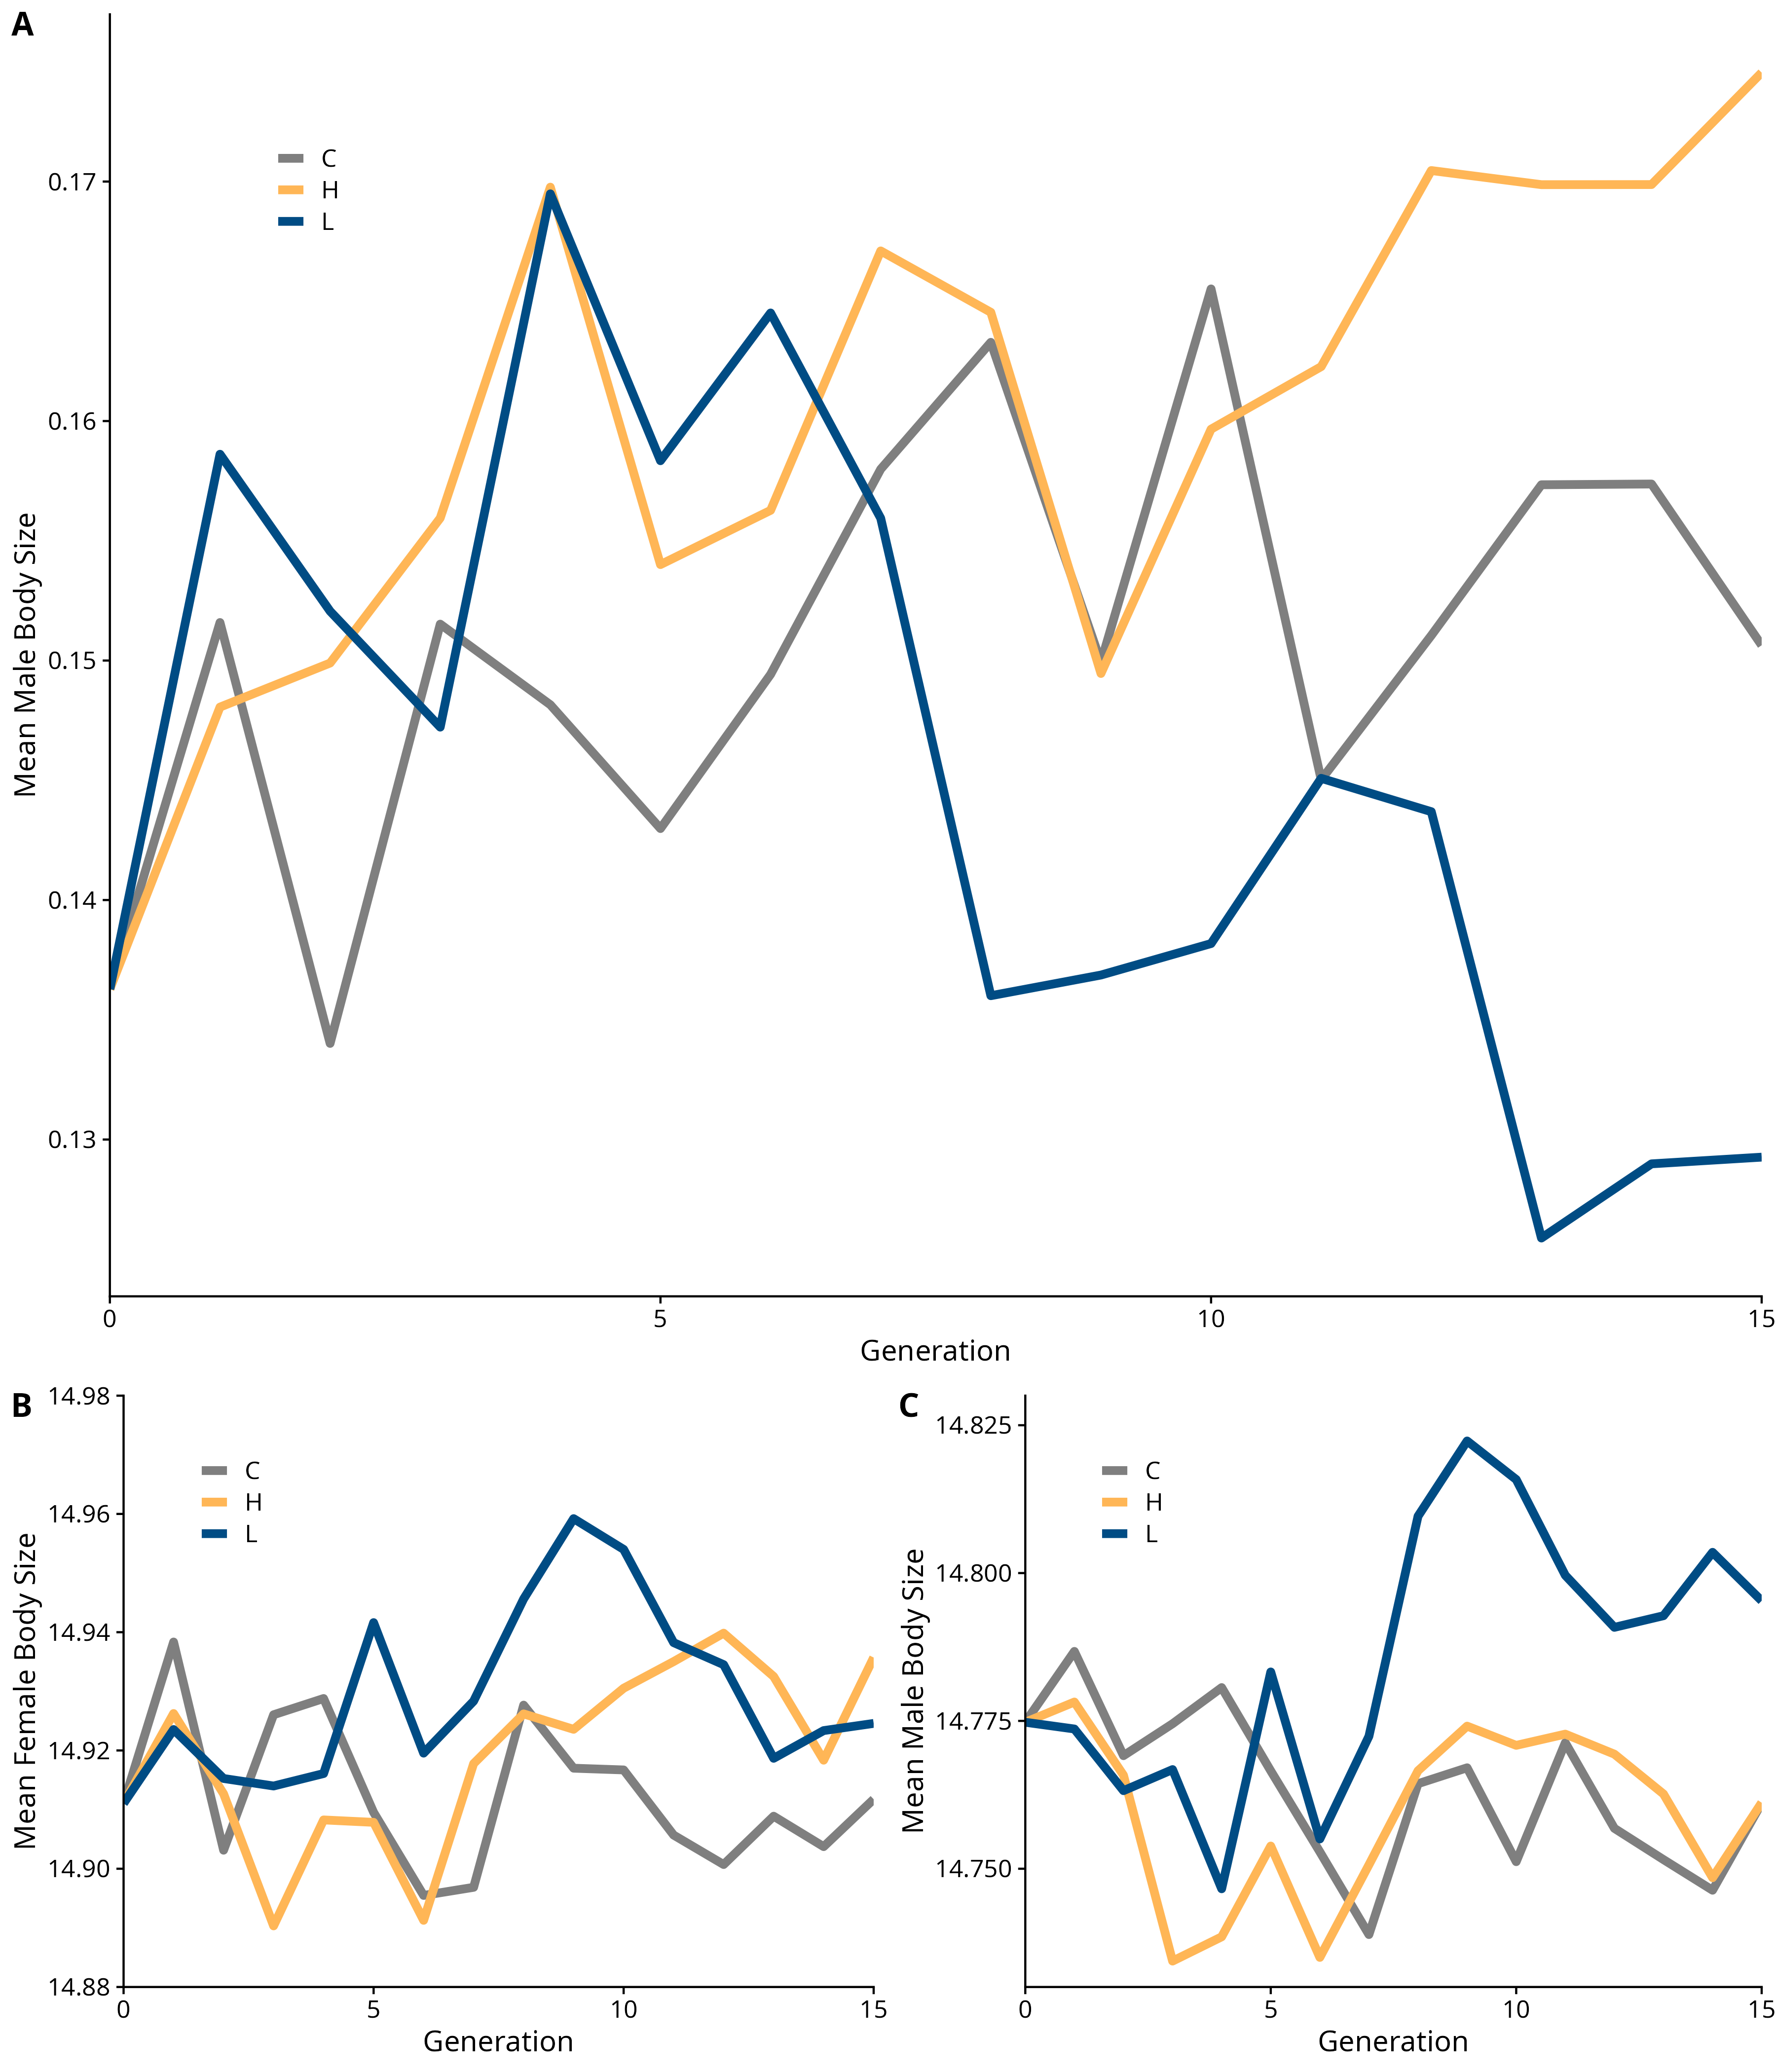
\includegraphics[alt = "Raw responses to selection on SSD.", width=0.8\textwidth]{rawplots.png}
    \caption{Raw responses to selection on SSD. (A) Changes in SSD. (B) Changes in female body size. (C) Changes in male body size. Points represent lineage means. These raw responses form the basis for the control-adjusted responses shown in Figure 2.4.}
    \label{fig:rawww}
\end{figure}
\clearpage

\begin{figure}
    \centering
    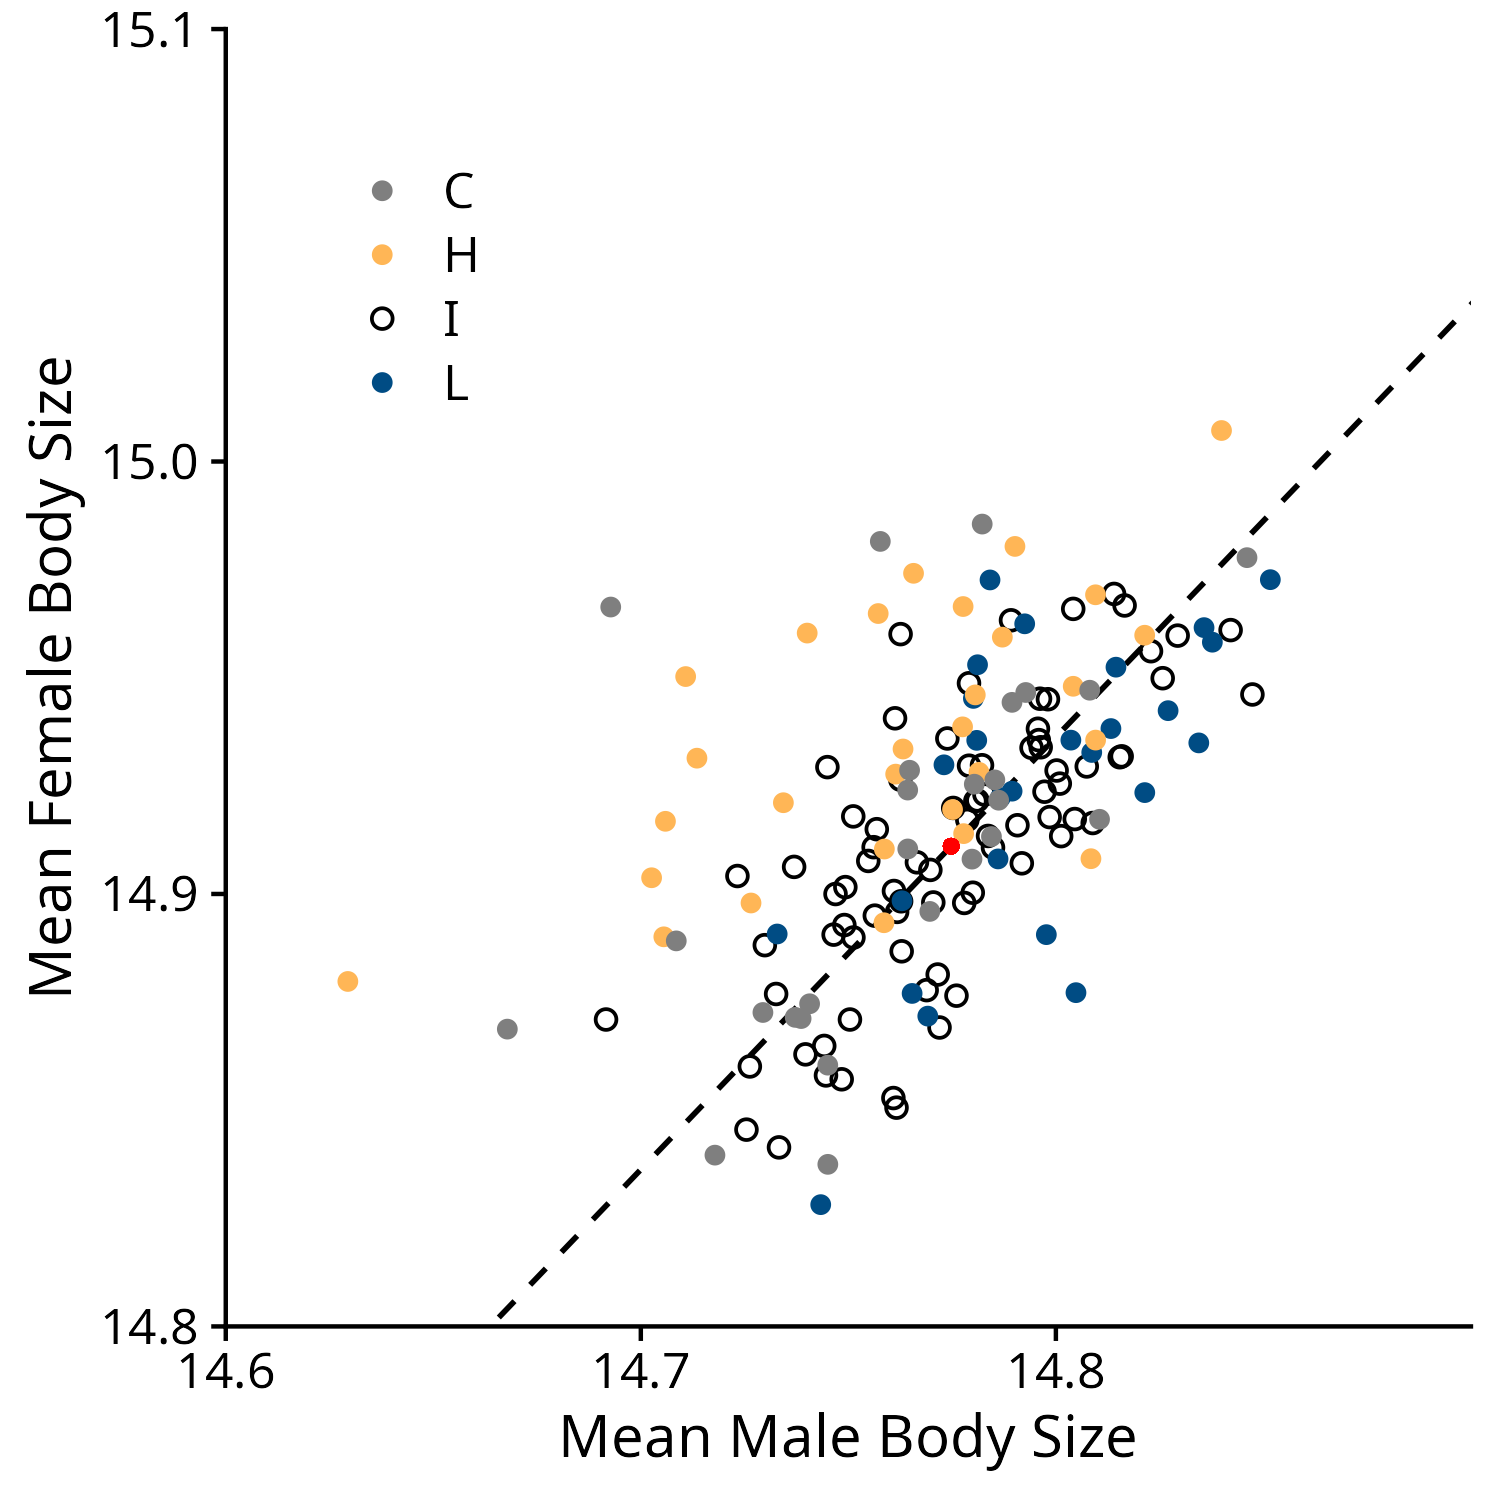
\includegraphics[alt = "Family mean sex specific body sizes plotted against one another for initial and final populations.", width=0.9\textwidth]{FvMpoint.png}
    \caption{Family mean sex specific body sizes plotted against one another for initial (open circle) and final (filled circle) populations. The red dot represents initial average SSD. The dotted line has a slope of 1. As points go further above this line SSD increases, and as they go further below SSD decreases.}
    \label{fig:FvMpoint}
\end{figure}
\clearpage

\begin{figure}
    \centering
    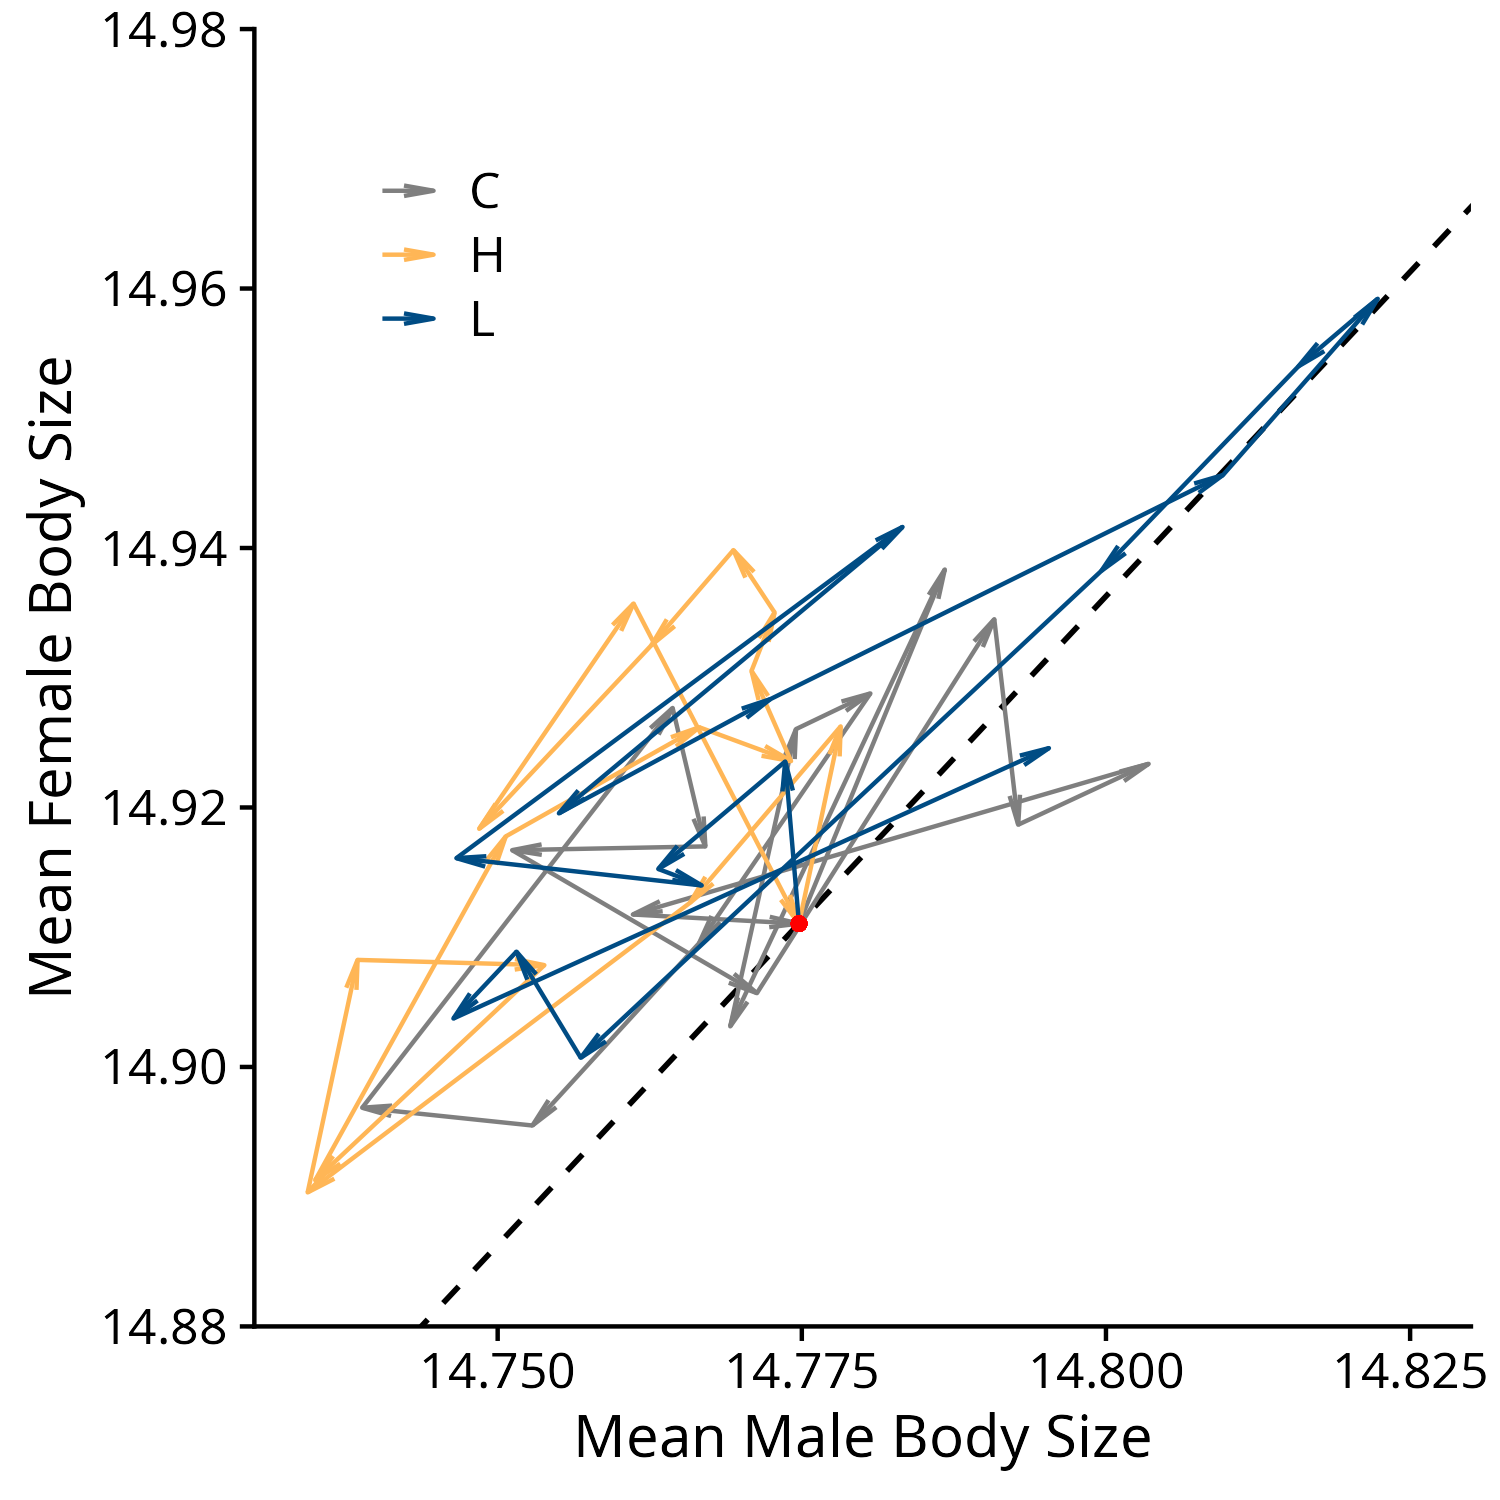
\includegraphics[alt = "Changes in generational mean sex-specific body sizes plotted against one another for each lineage.", width=0.9\textwidth]{FvMpath.png}
    \caption{Changes in generational mean sex-specific body sizes plotted against one another for each lineage. The red dot represents initial average SSD. The dotted line running through it has a slope of 1. As points go further above this line SSD increase, and as they go further below SSD decreases.}
    \label{fig:FvMpath}
\end{figure}
\clearpage

\begin{figure}
    \centering
    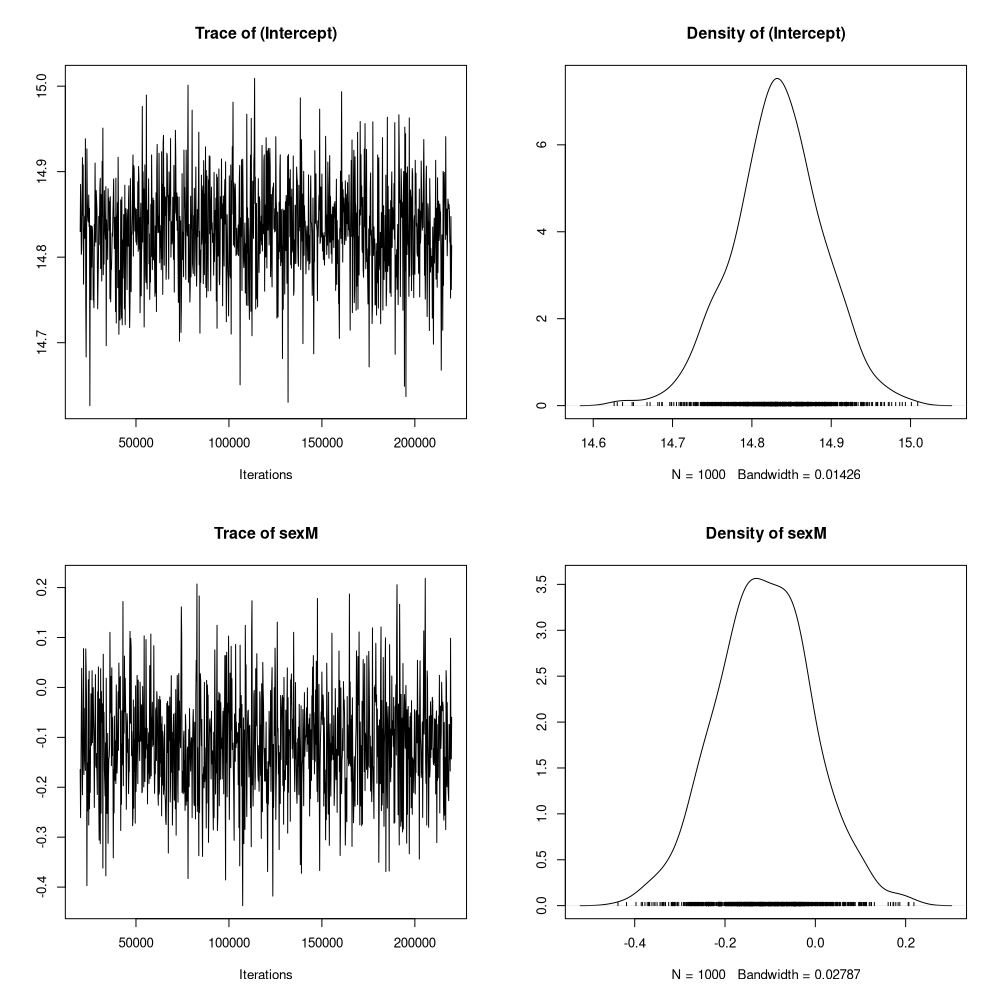
\includegraphics[alt = "Markov chain Monte Carlo generalized linear mixed model output part 1 of 3", width=1\textwidth]{MCMCGLMMplot1.png}
    \caption{Markov chain Monte Carlo generalized linear mixed model output from the MCMCglmm package (part 1 of 3) used to characterize variation in SSD among isogenized FVW lineages and estimate genetic variances for male and female body size. See Figures 5.5 and 5.6 for additional output.}
    \label{fig:mcmc1}
\end{figure}
\clearpage

\begin{figure}
    \centering
    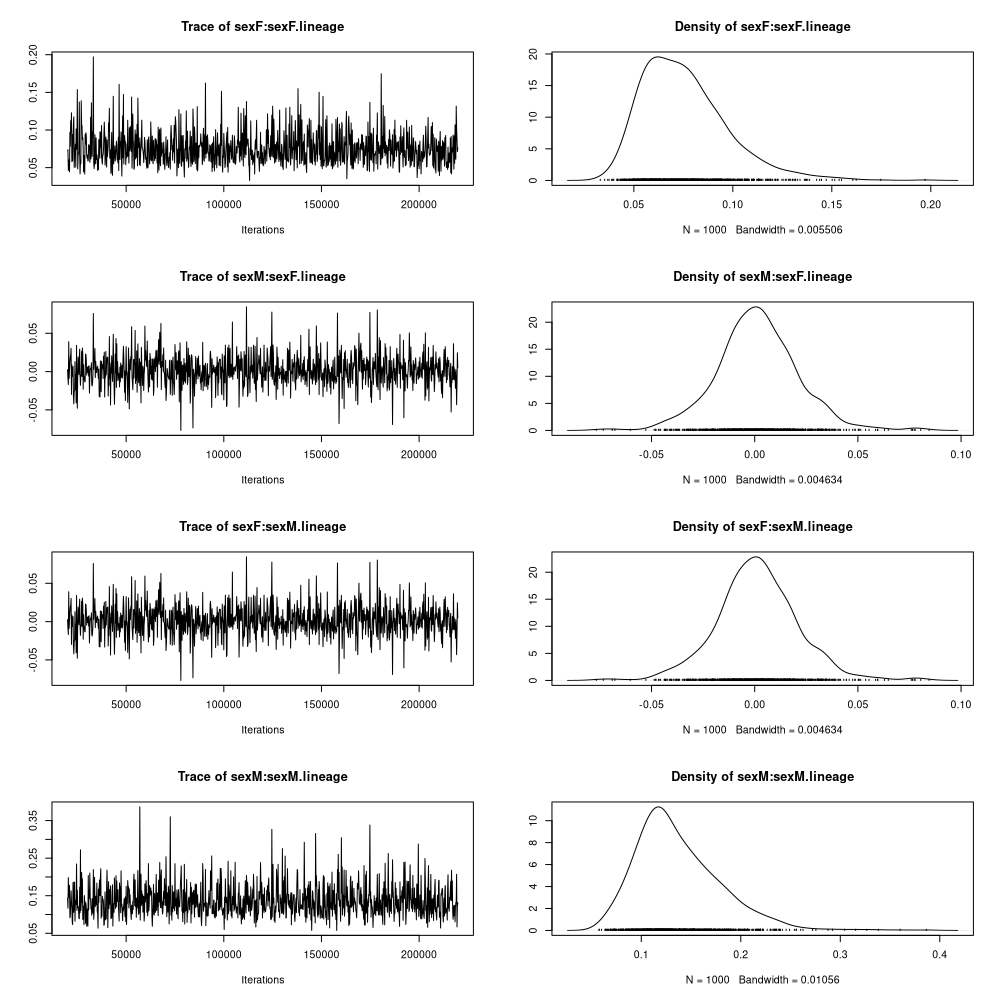
\includegraphics[alt = "Markov chain Monte Carlo generalized linear mixed model output part 2 of 3", width=1\textwidth]{MCMCGLMMplot2.png}
    \caption{Markov chain Monte Carlo generalized linear mixed model output from the MCMCglmm package (part 2 of 3). Continuation of analysis shown in Figure 5.4.}
    \label{fig:mcmc2}
\end{figure}
\clearpage

\begin{figure}
    \centering
    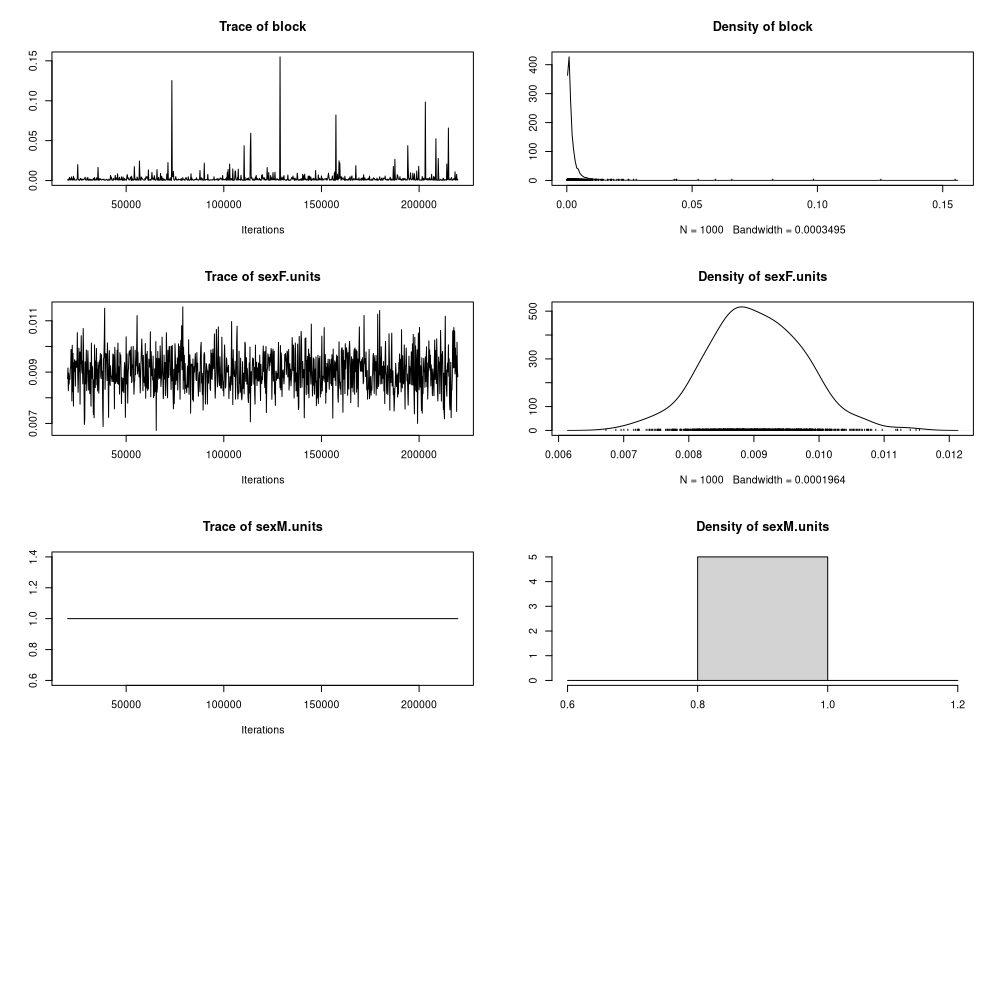
\includegraphics[alt = "Markov chain Monte Carlo generalized linear mixed model output part 3 of 3", width=1\textwidth]{MCMCGLMMplot3.png}
    \caption{Markov chain Monte Carlo generalized linear mixed model output from the MCMCglmm package (part 3 of 3). Continuation of analysis shown in Figures 5.4 and 5.5.}
    \label{fig:mcmc3}
\end{figure}
\clearpage

\tagpdfsetup{table/header-rows={1}}
\begin{table}
    \centering
    \caption{Counts of \textit{D. melanogaster} individuals in each extraction pool.}
    \begin{tabular}{cccc}
        Sample ID & Lineage & Sex & Count \\ \hline
        HMA1 & High SSD & Male & 18 \\ \hline
        HMA2 & High SSD & Male & 17 \\ \hline
        HMB1 & High SSD & Male & 17 \\ \hline
        HMB2 & High SSD & Male & 17 \\ \hline
        HFA1 & High SSD & Female & 18 \\ \hline
        HFA2 & High SSD & Female & 17 \\ \hline
        HFB1 & High SSD & Female & 17 \\ \hline
        HFB2 & High SSD & Female & 17 \\ \hline
        LMA1 & Low SSD & Male & 15 \\ \hline
        LMB12 & Low SSD & Male & 14 \\ \hline
        LMB2 & Low SSD & Male & 14 \\ \hline
        LFA1 & Low SSD & Female & 14 \\ \hline
        LFA2 & Low SSD & Female & 13 \\ \hline
        LFB1 & Low SSD & Female & 13 \\ \hline
        LFB2 & Low SSD & Female & 13 \\ \hline
        CMA1 & Control & Male & 19 \\ \hline
        CMA2 & Control & Male &	19 \\ \hline
        CMB1 & Control & Male &	18 \\ \hline
        CMB2 & Control & Male &	18 \\ \hline
        CFA1 & Control & Female & 21 \\ \hline
        CFA2 & Control & Female & 21 \\ \hline
        CFB1 & Control & Female & 20 \\ \hline
        CFB2 & Control & Female & 20 \\ \hline
        OMA1 & Initial & Male &	24 \\ \hline
        OMA2 & Initial & Male &	24 \\ \hline
        OMB1 & Initial & Male &	24 \\ \hline
        OMB2 & Initial & Male &	24 \\ \hline
        OMC	& Initial & Male &	24 \\ \hline
        OFA1 & Initial & Female & 24 \\ \hline
        OFA2 & Initial & Female & 24 \\ \hline
        OFB1 & Initial & Female & 24 \\ \hline
        OFB2 & Initial & Female & 24 \\ \hline
        OFC	& Initial & Female & 24 \\ \hline
    \end{tabular}
    \label{tab:poolcounts}
\end{table}
\clearpage

\begin{figure}
    \centering
    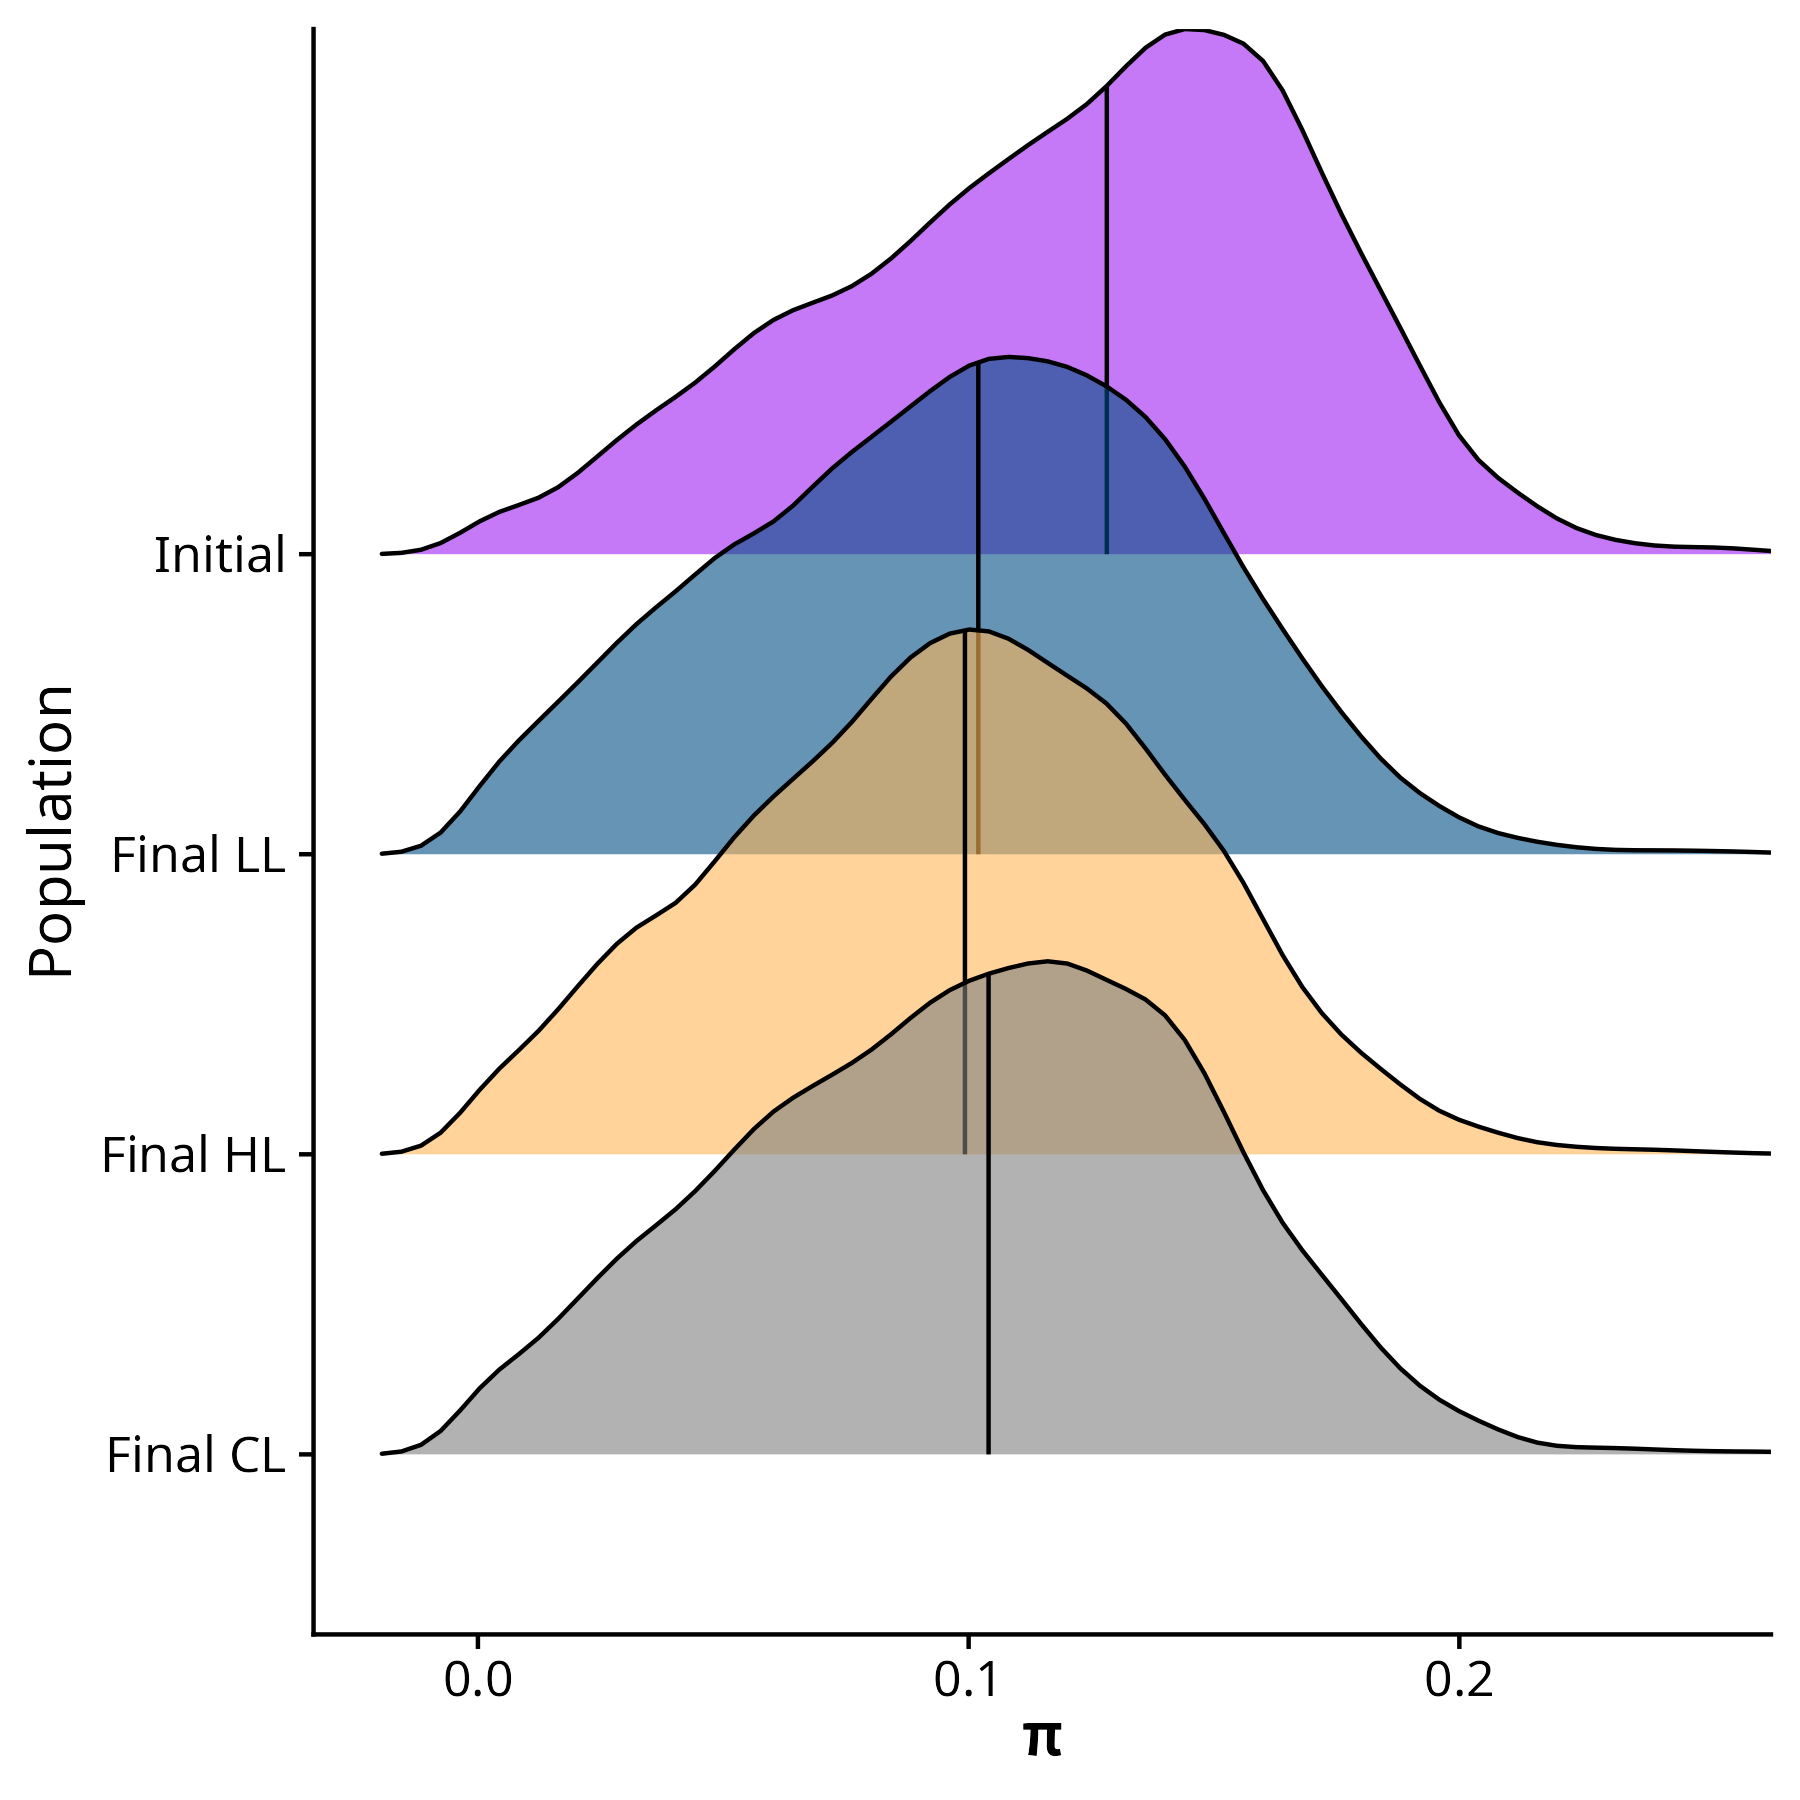
\includegraphics[alt = "Nucleotide diversity of initial and final populations.", width=1\linewidth]{piplot.png}
    \caption{Nucleotide diversity (\(\pi\)) between the initial (FVW) and final selected populations (CL, HL, LL). Nucleotide diversity was calculated from pooled sequencing data in 10 kb windows across the genome.}
    \label{fig:piplot}
\end{figure}
\clearpage

\begin{figure}
    \centering
    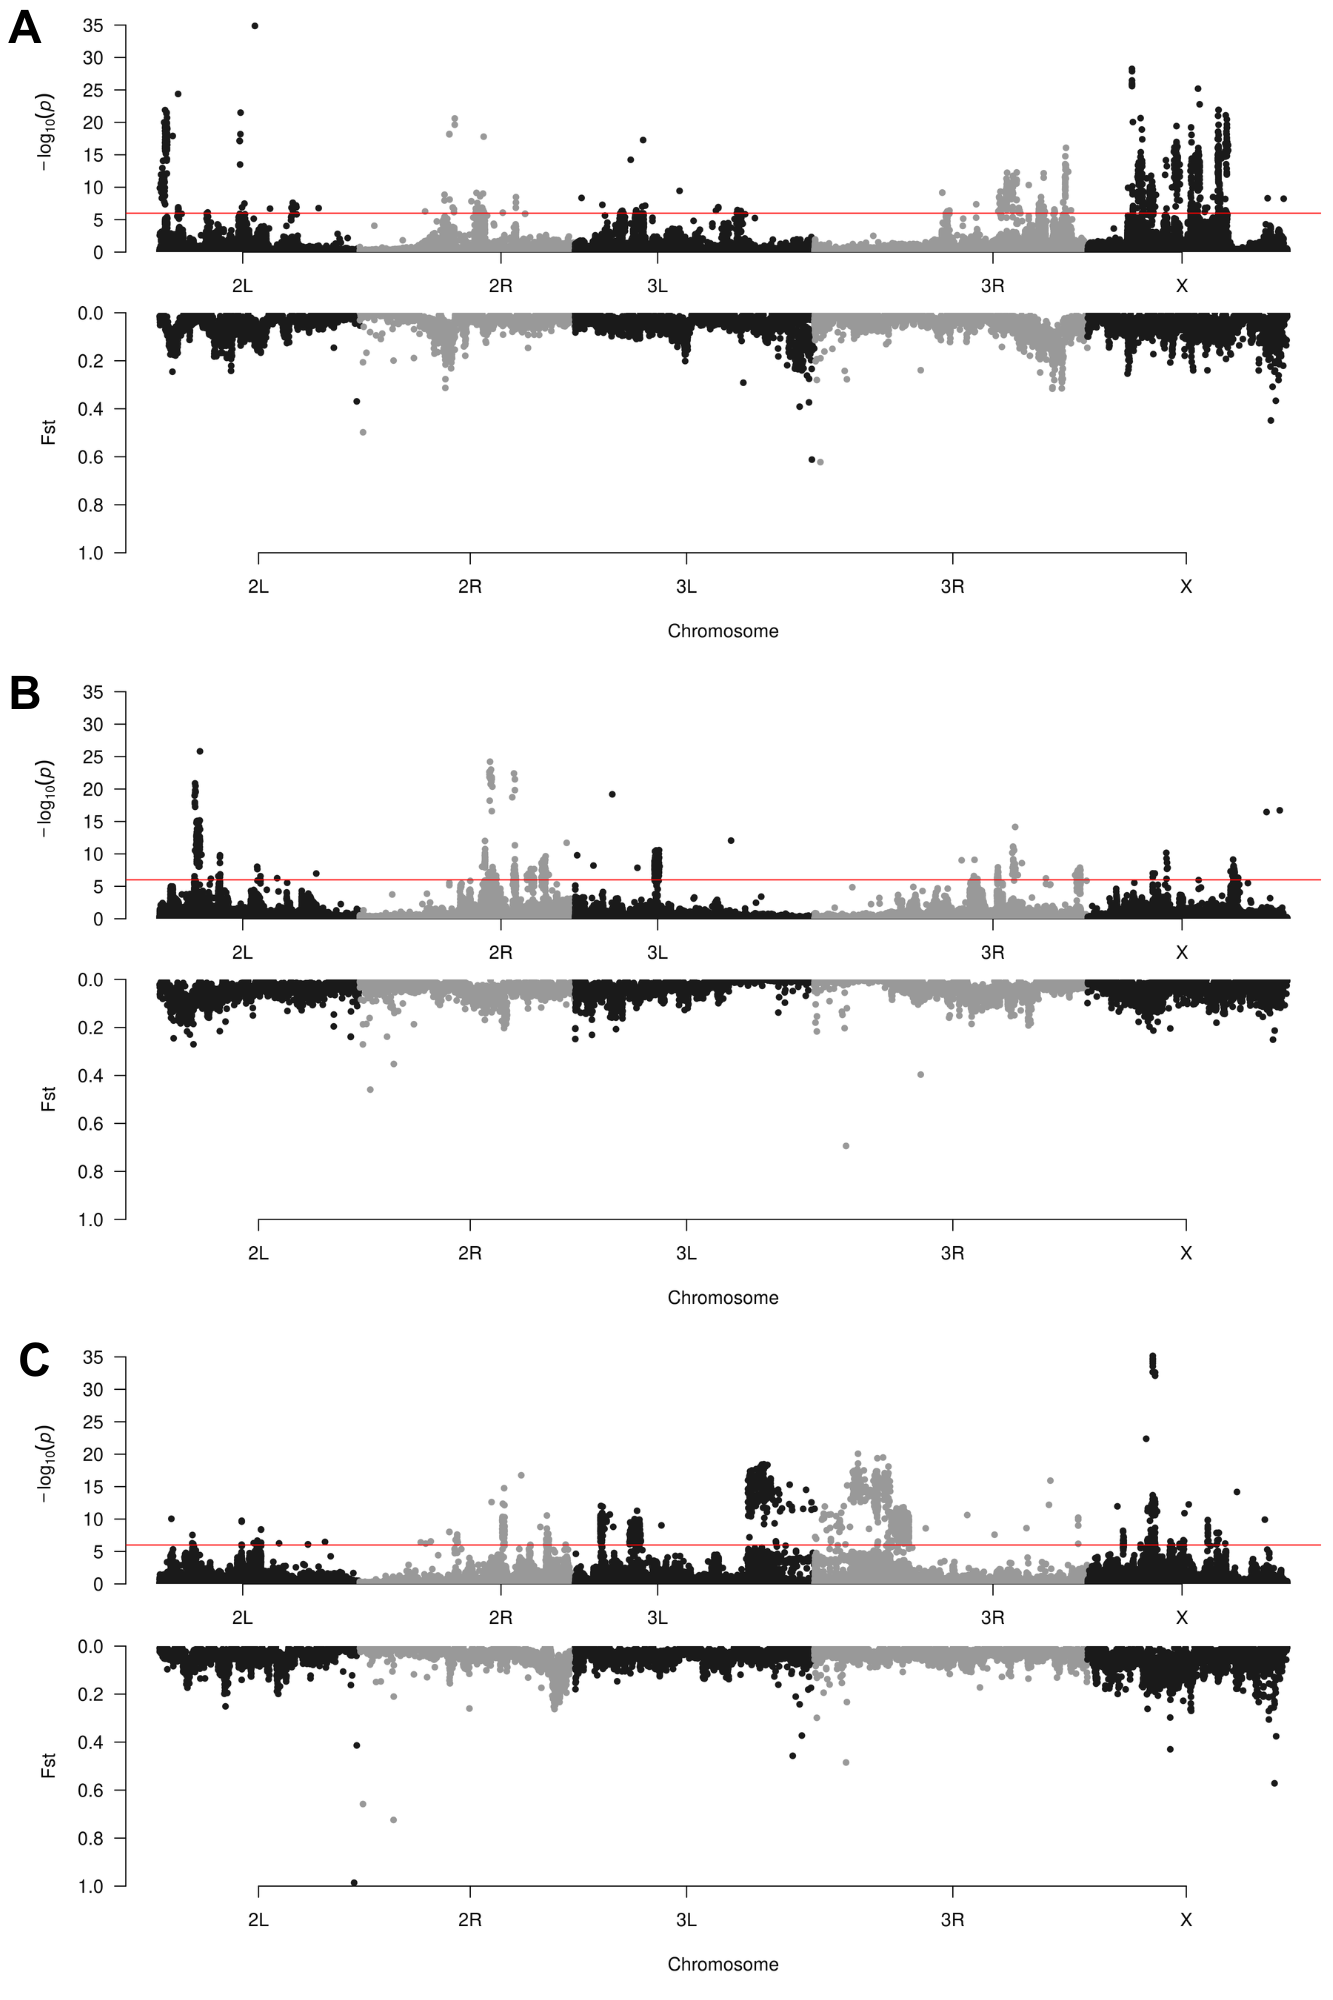
\includegraphics[alt = "Adapted chi-square test against FST", width=0.75\linewidth]{Fst.png}
    \caption{Adapted chi-square test results (upper panels) and windowed (10kb) \(F_{ST}\) (lower panels) for each lineage; (A) CL, (B) HL, and (C) LL. Red line represents 10e-6, the threshold for significance used in this study.}
    \label{fig:chiFST}
\end{figure}

%CHAPTER 4
\clearpage
\begin{figure}
    \centering
    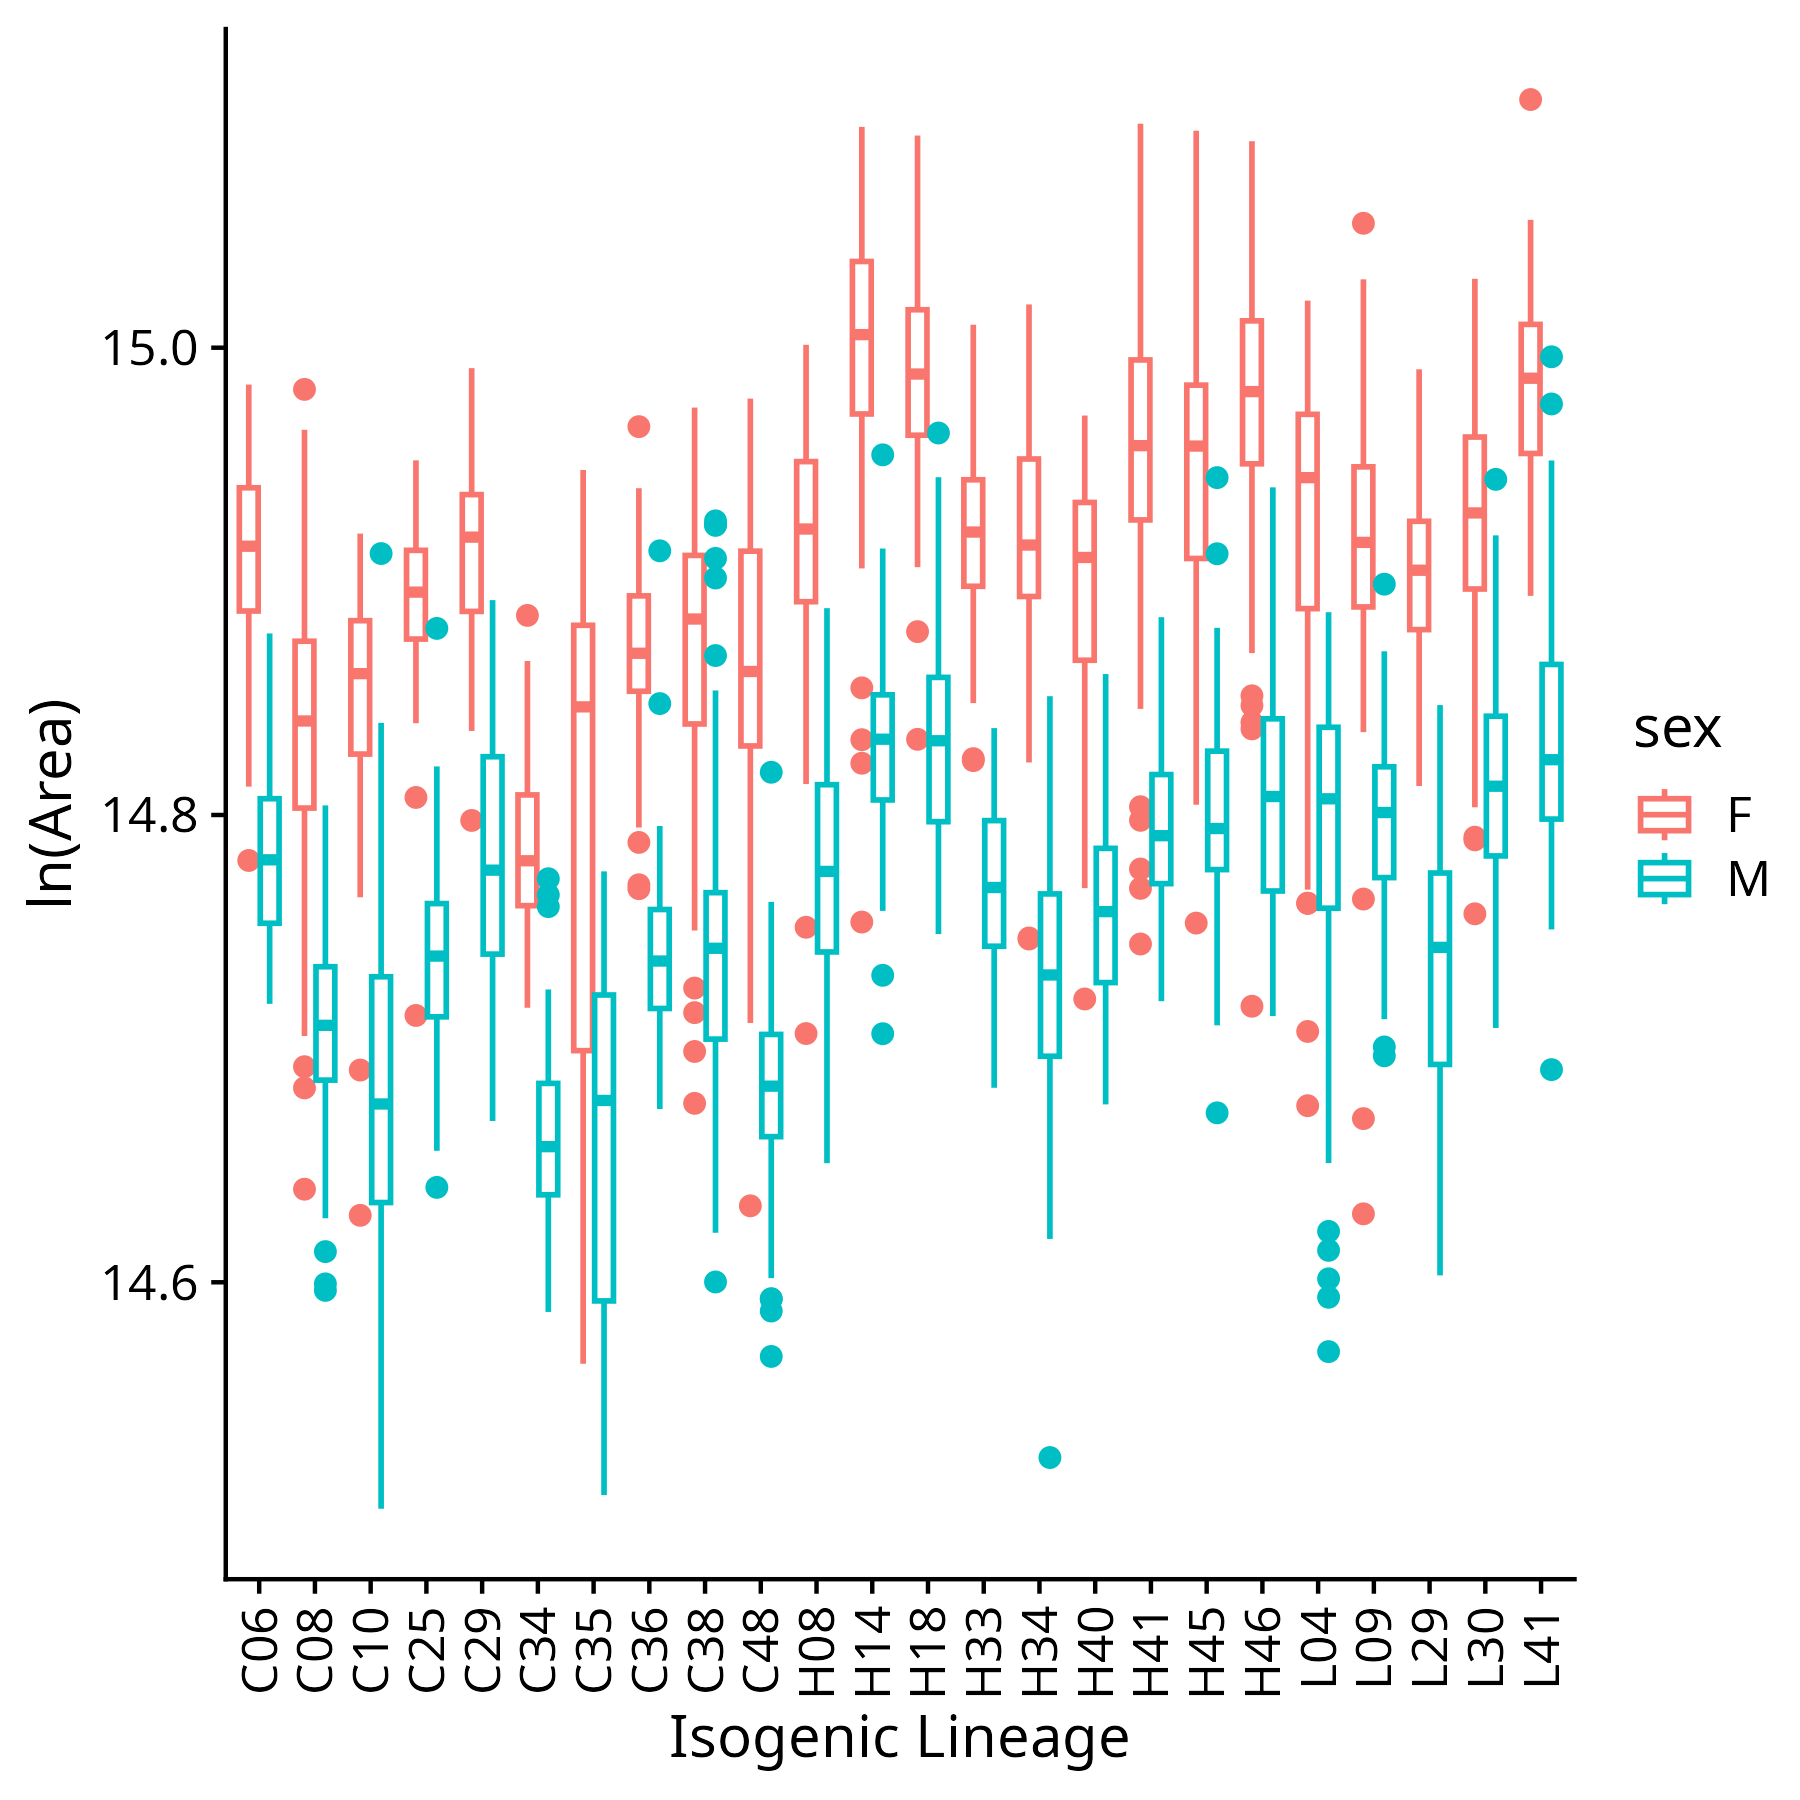
\includegraphics[alt = "Distribution of size by sex for each isogenic lineage.", width=1\linewidth]{isoSSDbySex.png}
    \caption{Distribution of size by sex for each isogenic lineage.}
    \label{fig:isoSSDbySex}
\end{figure}

\clearpage
\begin{figure}
    \centering
    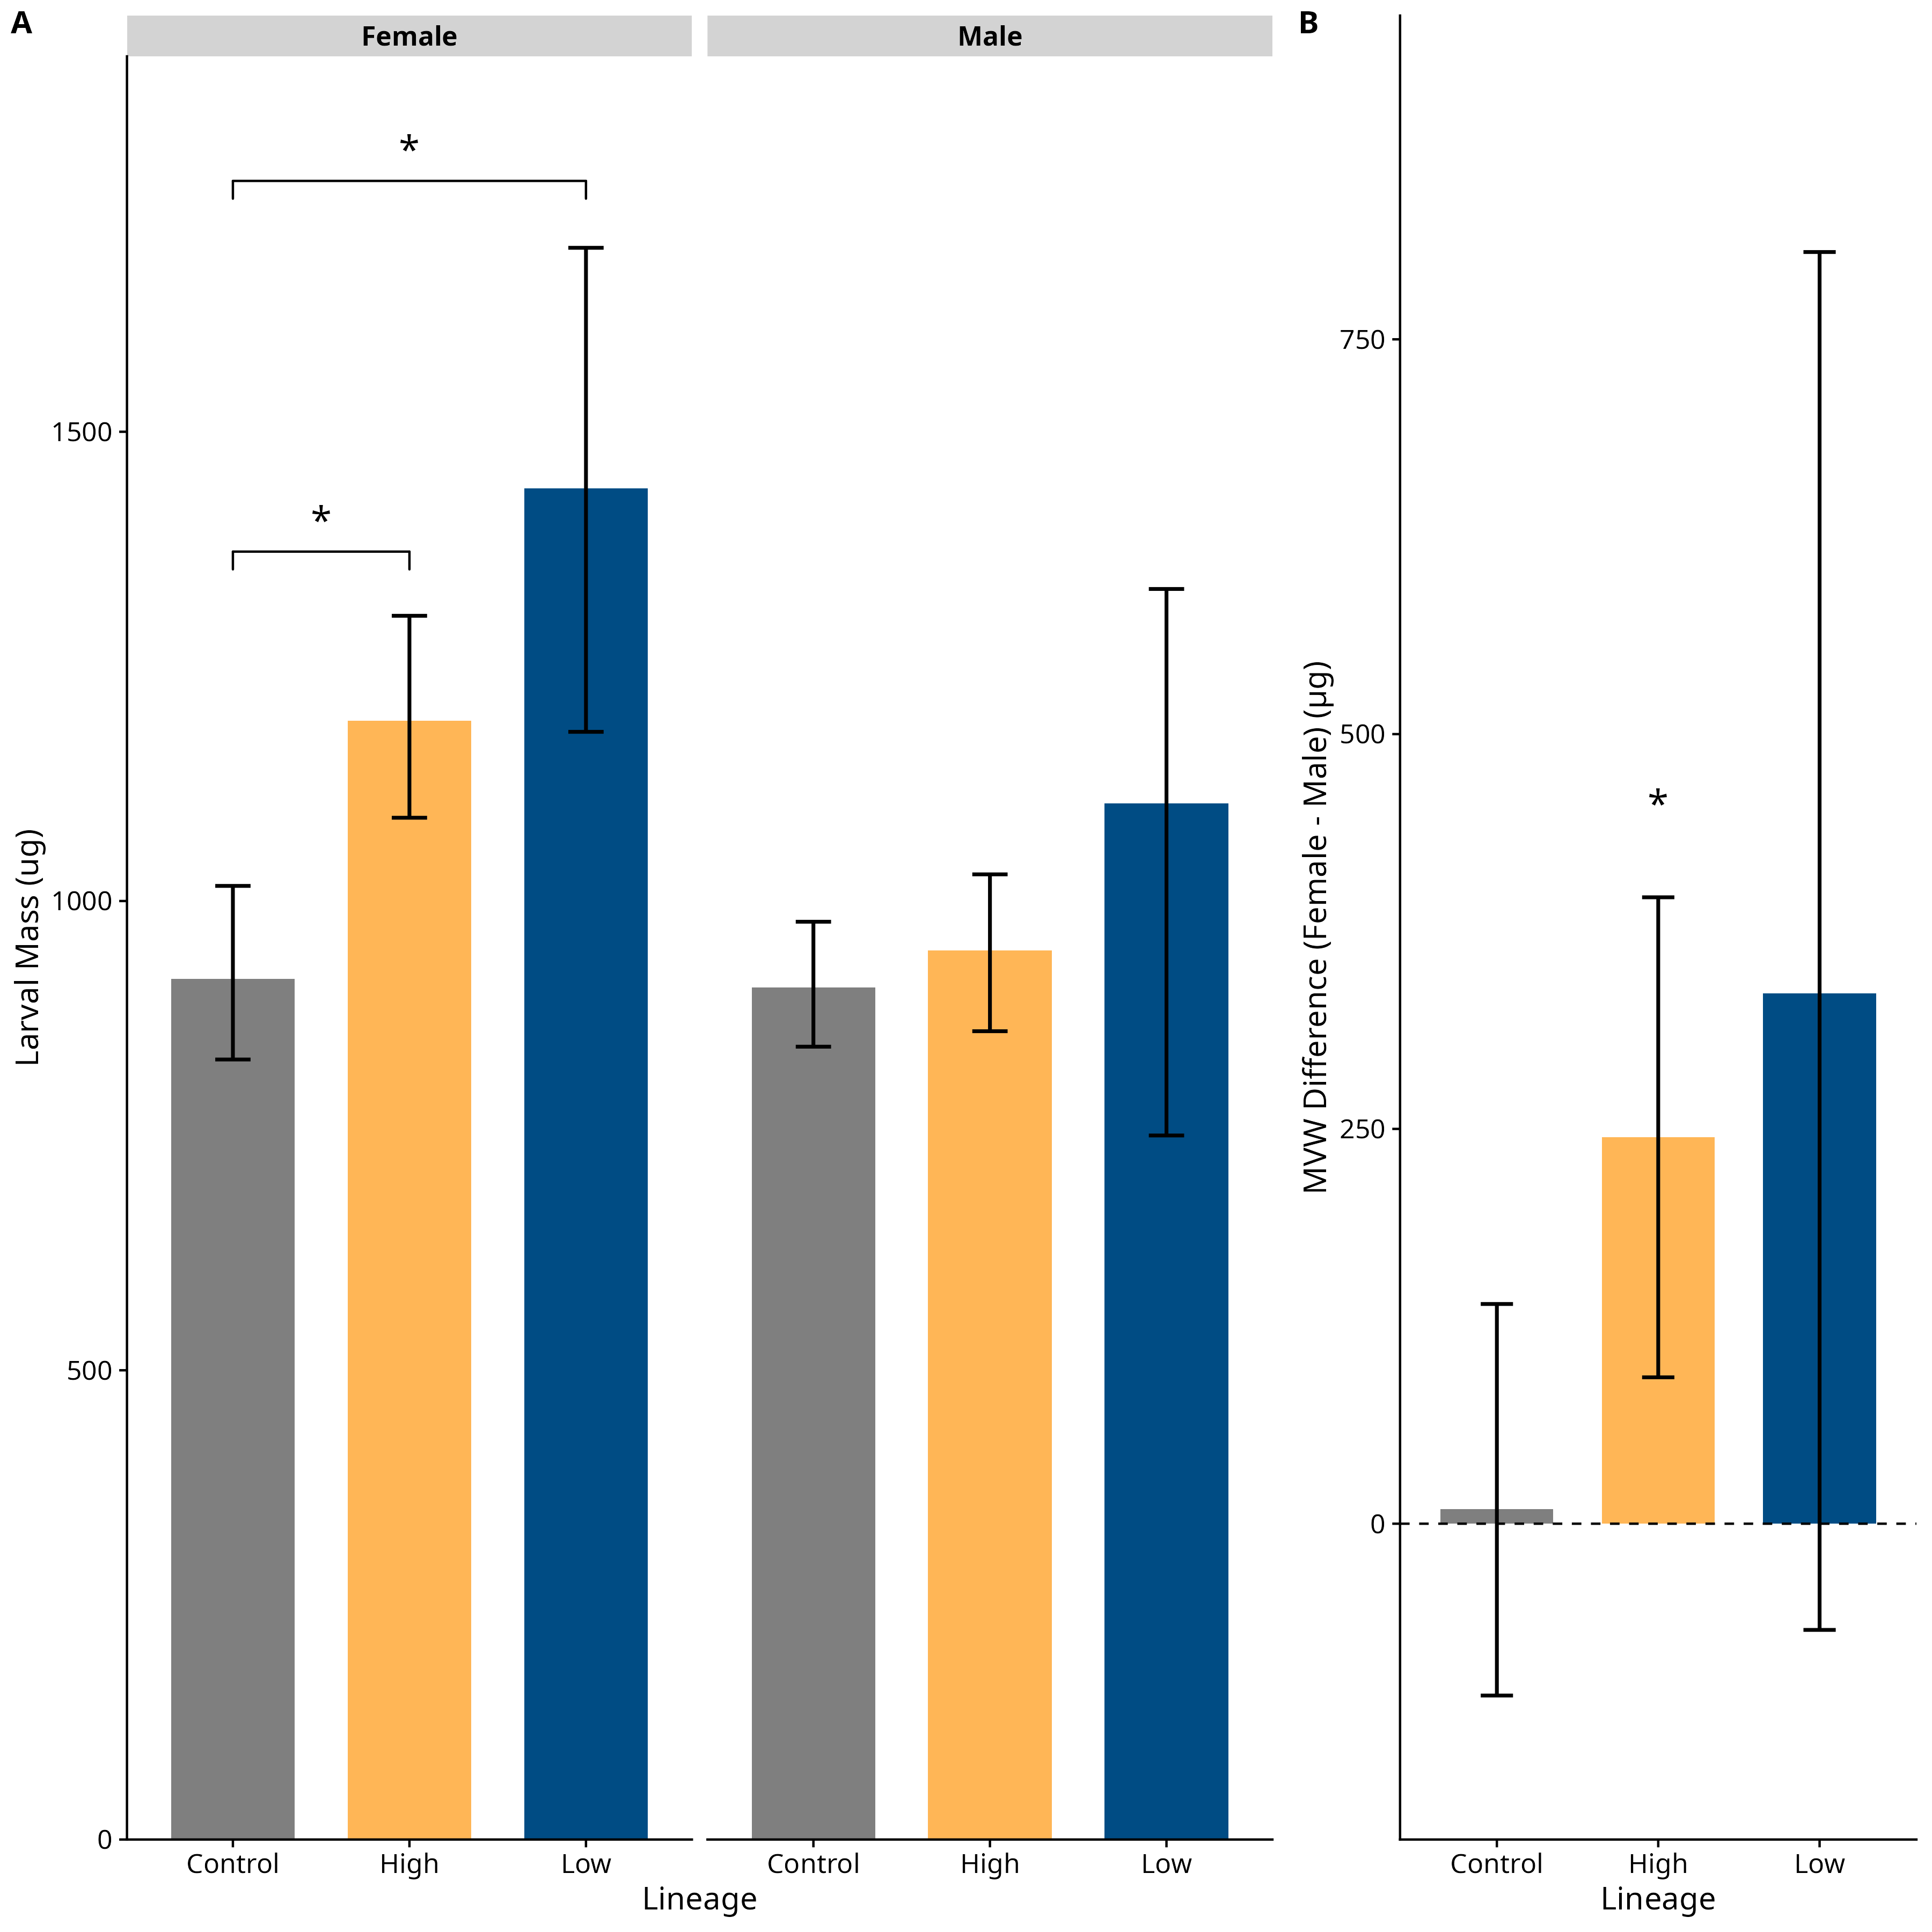
\includegraphics[alt = "Unadjusted minimal viable weight.", width=1\linewidth]{MVW_sup.png}
    \caption{Minimal viable weight (MVW) across lineages and sexes. Asterisks denote significant sex differences within each lineage, determined if Bonferroni adjusted confidence interval of difference between groups did not contain zero. (A) MVW estimates with whiskers reflecting the 95\% credibility intervals. (B) Differences in MVW between the sexes within lineages.}
    \label{fig:MVWsup}
\end{figure}

\clearpage
\begin{figure}
    \centering
    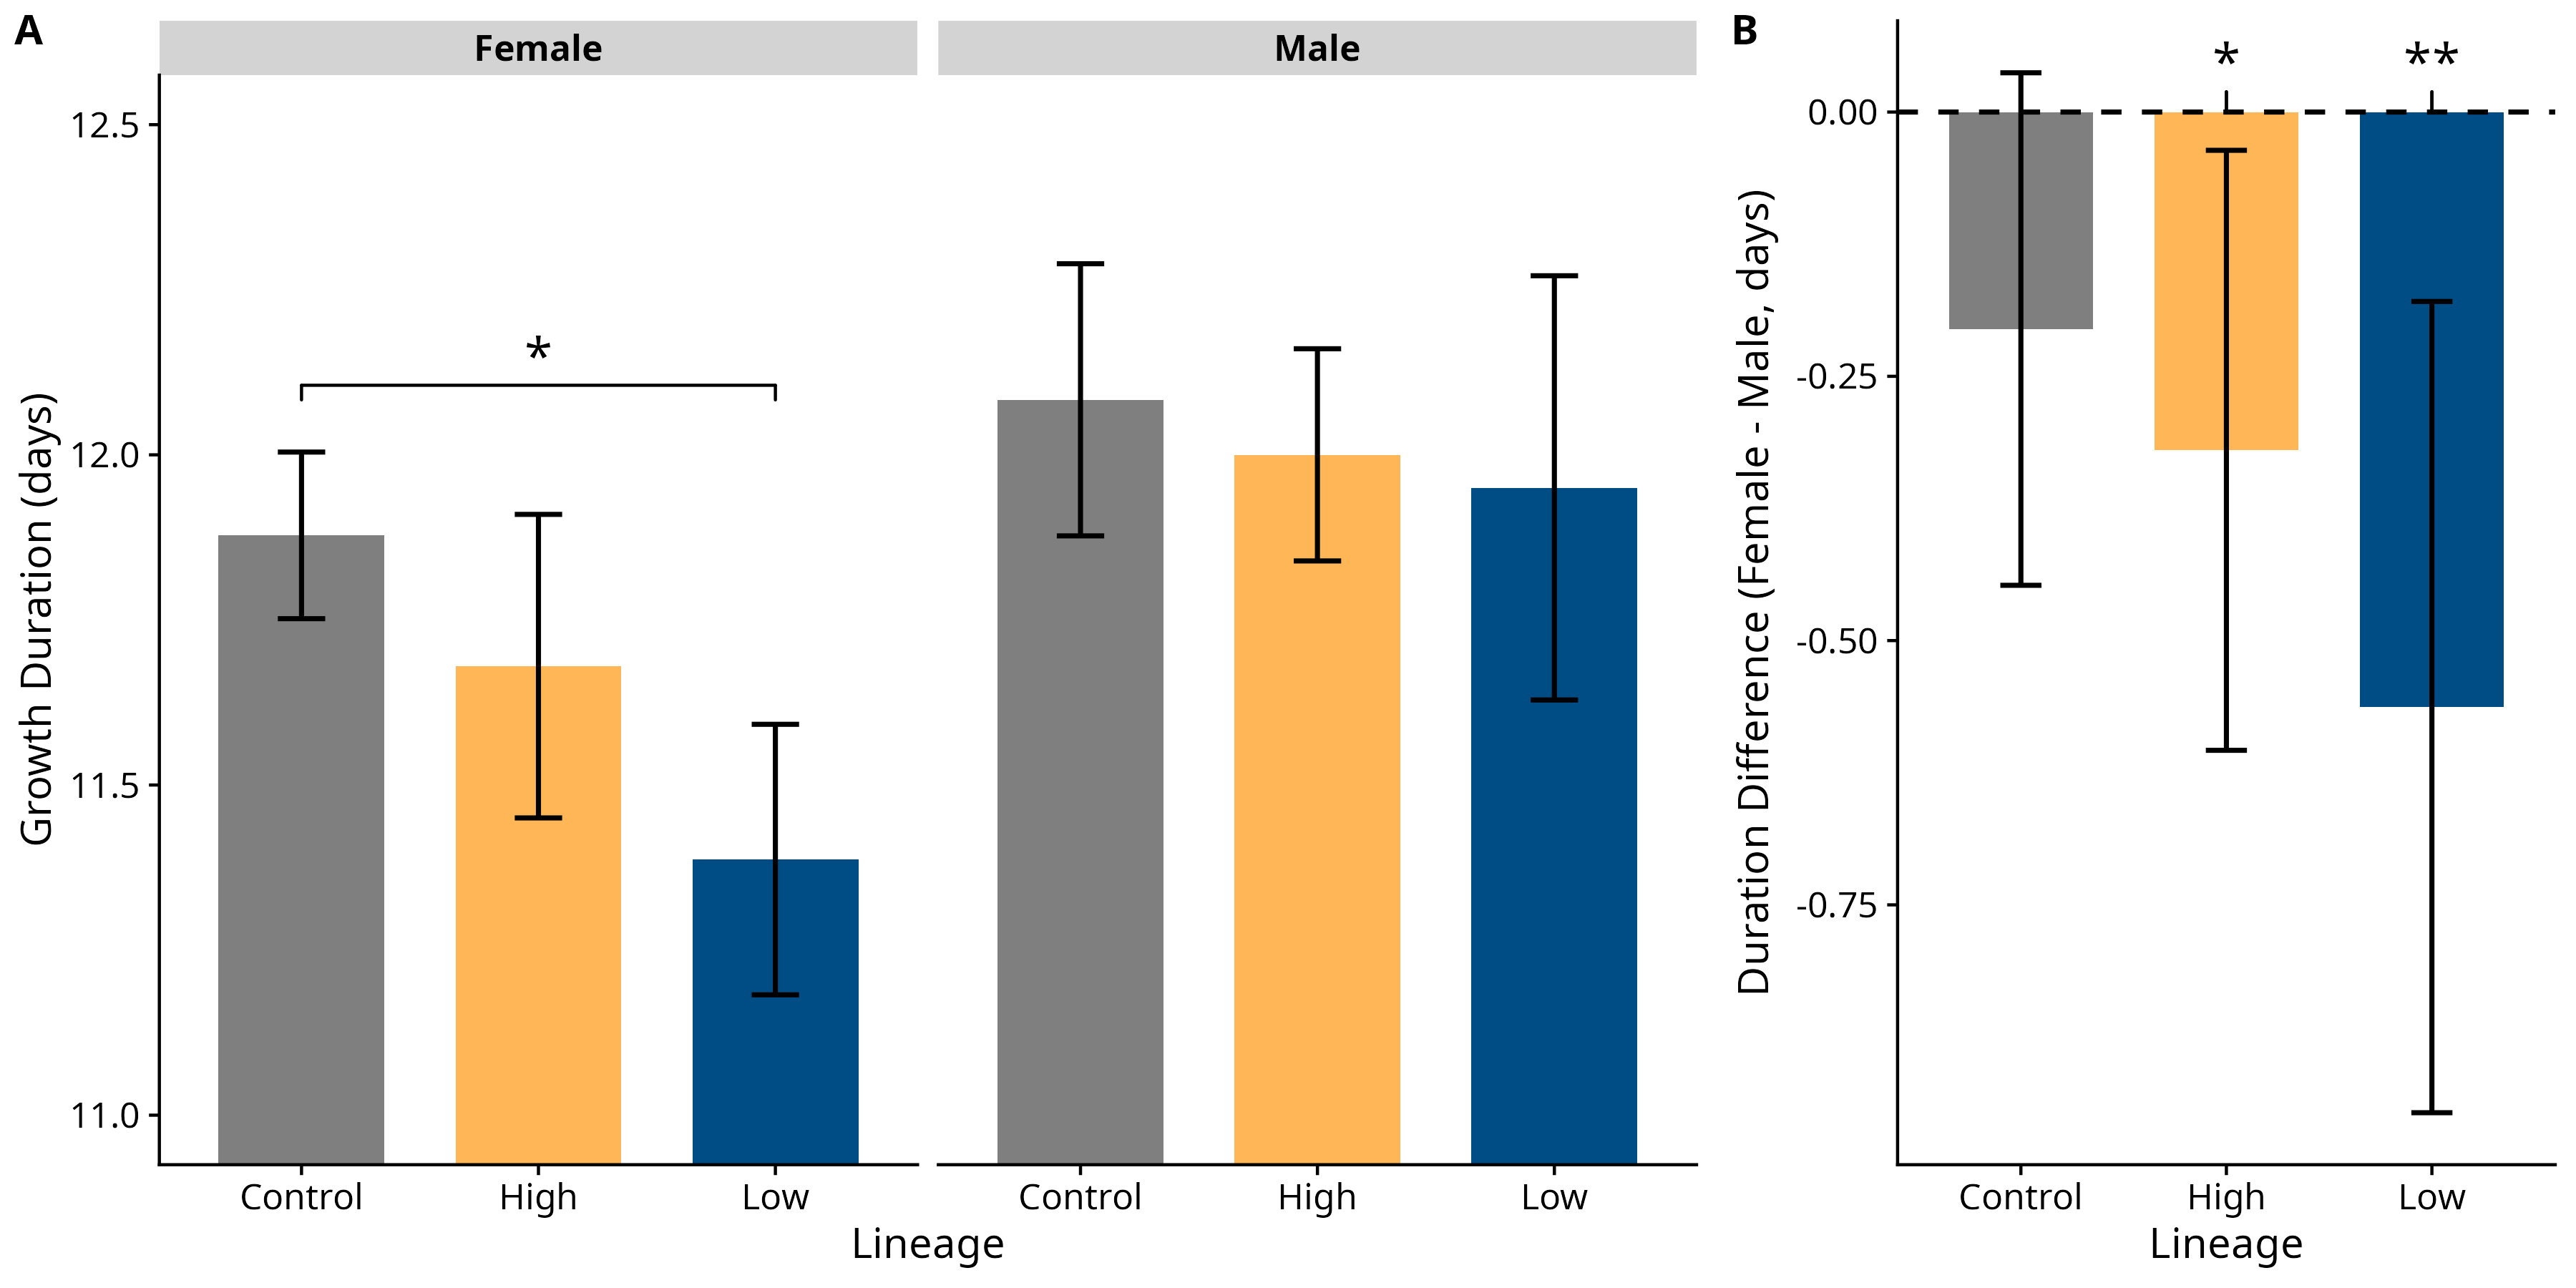
\includegraphics[alt = "Unadjusted duration of growth.", width=1\linewidth]{durationCombined.png}
    \caption{Duration of growth. (A) By lineage and sex. LF vs CF are significantly different from one another (ANOVA: F\(_{2,94}\) = 8.63, $P$ < 0.001). Male developmental timing did not differ across lineages ($P$ = 0.71). (B) Difference between the duration of growth of the sexes. Welch t-testing found that CL sexes did not differ significantly ($P$ = 0.09), while the selected lineages had significant differences in developmental time between the sexes (HL $P$ = 0.02, LL $P$ < 0.01) with females had a shorter growth duration than their male counterparts.}
    \label{fig:durCombined}
\end{figure}

\clearpage
\begin{figure}[t!]
    \centering
    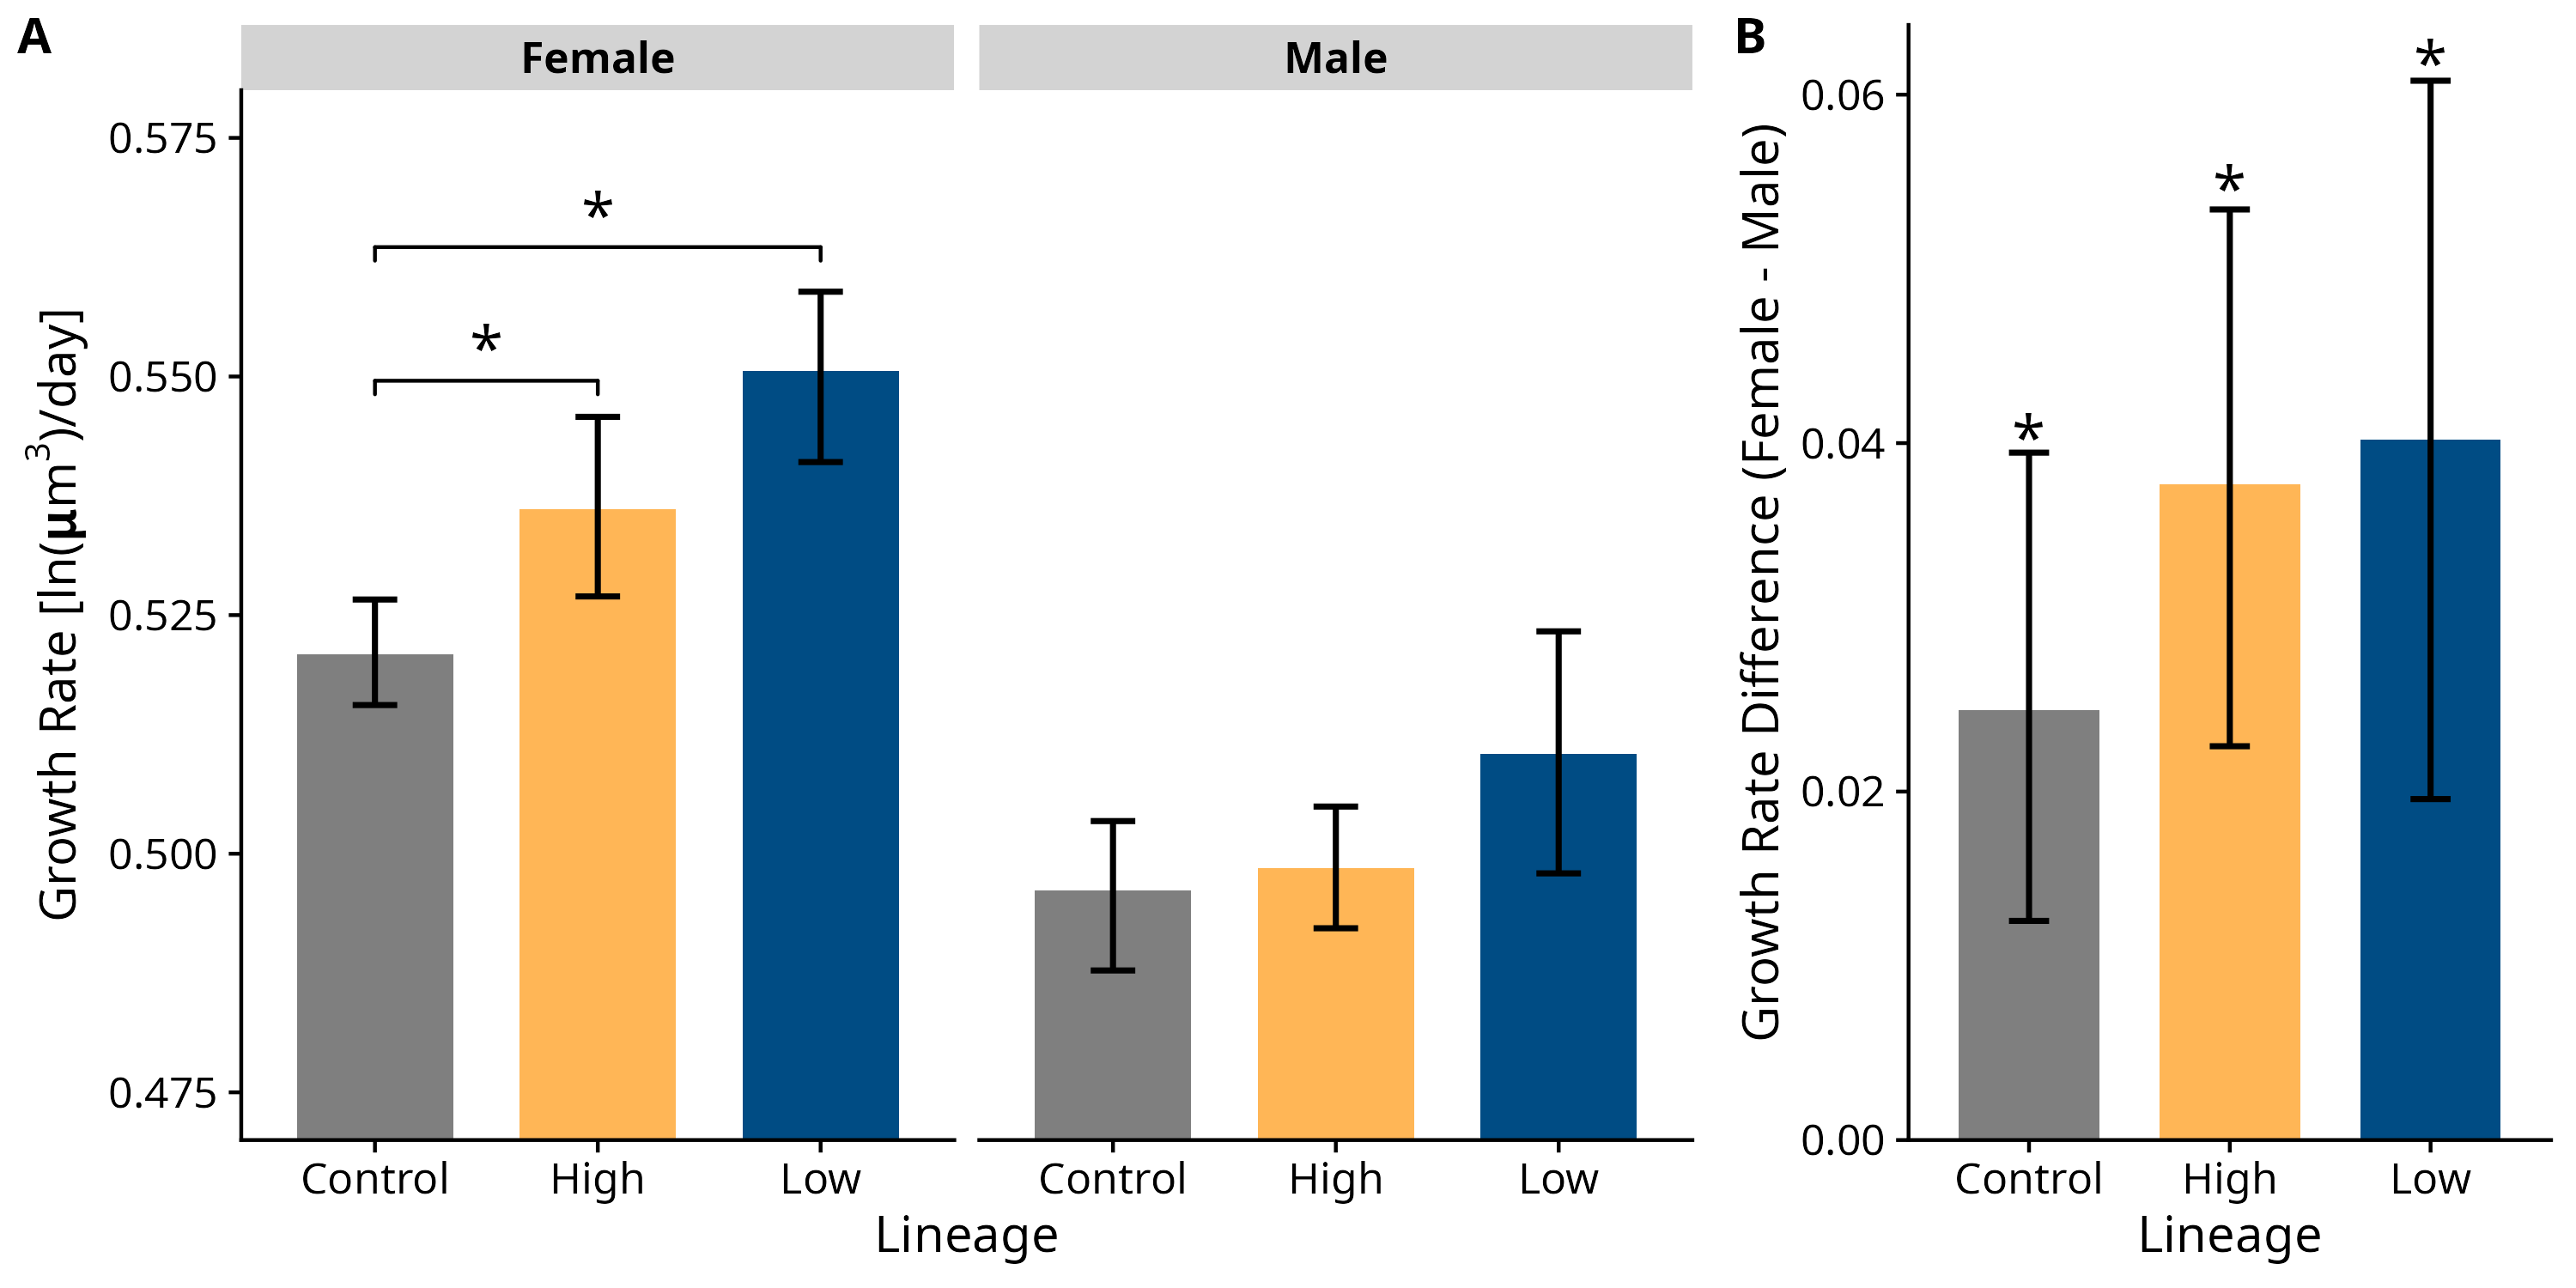
\includegraphics[alt = "Estimated growth rates across lineages.", width=1\linewidth]{growth_rate_combined.png}
    \caption{Estimated growth rates across lineages. Asterisks denote significant sex differences within each lineage, determined if Bonferroni adjusted confidence interval of difference between groups did not contain zero. (A) Growth rates faceted by sex. Females of selected lineages differed significantly from controls, while males of all lineages did not. (B) Within lineage comparisons. The sexes of each lineage differed significantly, with females having a faster growth rate in each lineage.}
    \label{fig:growthcombinedunadj}
\end{figure}

\clearpage
\noindent
\textbf{Published Figure Usage:} Published figures from both Shingleton and Vea (2023) and Testa et al. (2013) were used in this dissertation. Both articles are open access, and as such their usage falls under the Creative Commons.

\begin{figure}
    \centering
    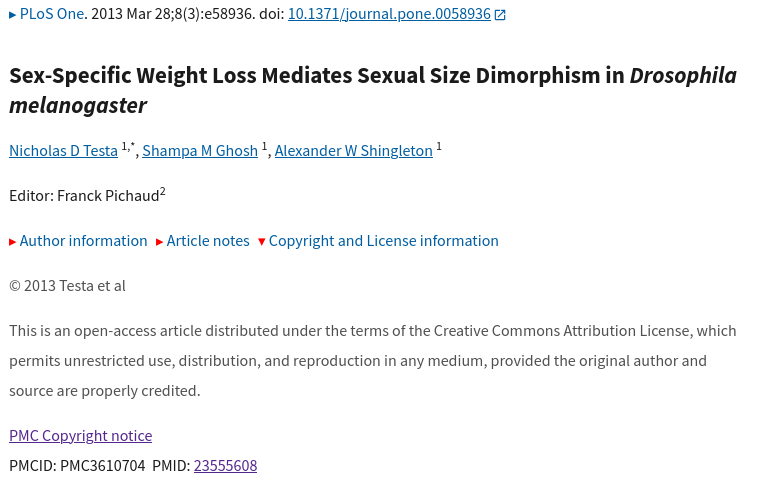
\includegraphics[alt = "Screenshot of from PMC's website showing Testa et al. (2013) falls under the Creative Commons.", width=1\linewidth]{testaetalcopyright.png}
    \caption{Screenshot of from PMC's website showing Testa et al. (2013) falls under the Creative Commons.}
    \label{fig:testacopy}
\end{figure}

\begin{figure}
    \centering
    
\includegraphics[alt = "Screenshot of from Elsevier's website showing Shingleton and Vea (2023) falls under the Creative Commons.", width=1\linewidth]{shingletonandveacopyright.png}
    \caption{Screenshot of from Elsevier's website showing Shingleton and Vea (2023) falls under the Creative Commons.}
    \label{fig:veacopy}
\end{figure}


\clearpage
\noindent
\textbf{AI Statement}
Generative AI was used when adapting Audet et al.'s (2024) bioinfomatics pipeline to adjust for version related issues and adjust for differences in experimental design.

\clearpage
\addcontentsline{toc}{chapter}{Vitae}

\centering
{\Huge\textbf{Elizabeth Agolli}}\\
\vspace{0.20cm}

PhD Candidate $\bullet$ Ecology \& Evolution\\
University of Illinois Chicago\\
lizagolli@gmail.com

\vspace{0.5cm}

\raggedright
{\Large\textbf{Education}}\hrulefill\\

\vspace{0.25cm}

\textbf{University of Illinois Chicago} \hfill \textit{Chicago, Illinois}\\
PhD Ecology \& Evolution \hfill \textit{Aug 2018 - present}\\

\vspace{0.25cm}

\textbf{St. John's University} \hfill \textit{Queens, New York}\\
BS Biology \hfill \textit{Sep 2014 - Dec 2017}\\

\vspace{0.5cm}

{\Large\textbf{Professional Experience}}\hrulefill\\

\tagpdfsetup{table/header-rows={0}}
\begin{table}[h]
    \raggedright
    \begin{tabular}{rl}
        2026 & \textbf{Graduate Teaching Assistant}, Biology, University of Illinois Chicago  \\
        2019-2023 & \textbf{Graduate Teaching Assistant}, Biology, University of Illinois Chicago  \\
        2011-2014 & \textbf{Undergraduate Research Assistant}, Biology, St. John's University
    \end{tabular}
\end{table}

{\Large\textbf{Awards}}\hrulefill\\

\tagpdfsetup{table/header-rows={0}}
\begin{table}[h]
    \raggedright
    \begin{tabular}{rl}
        2021 & \textbf{Teaching Award}, BIOS 310 Genetics, Dept. Biology
    \end{tabular}
\end{table}

{\Large\textbf{Presentations}}\hrulefill\\
\vspace{0.5cm}
\textbf{Talks}
\vspace{0.25cm}

\hangindent=1cm
Summer 2025. \textit{Using Artificial Selection to Uncover the Genetic Regulation of Sexual Size Dimorphism in D. melanogaster}. UIC Biology Symposium, Chicago, Illinois

\vspace{0.25cm}

\hangindent=1cm
Summer 2024. \textit{Using Artificial Selection to Uncover the Genetic Regulation of Sexual Size Dimorphism in D. melanogaster}. UIC Biology Symposium, Chicago, Illinois

\vspace{0.5cm}

\textbf{Posters}

\vspace{0.25cm}

\hangindent=1cm
Fall 2023. \textit{Sexual Size Dimorphism: Genetic Insights from Artificial Selection in Drosophila melanogaster}. Annual \textit{Drosophila} Research Conference, Chicago, Illinois

\vspace{0.25cm}

\hangindent=1cm
Fall 2022. \textit{Preliminary Results of Artificial Selection on Sexual Size Dimorphism}. Midwest \textit{Drosophila} Conference, Chicago, Illinois

\vspace{0.25cm}

\hangindent=1cm
Summer 2020. \textit{Sexual size dimorphism in the anterior legs of Drosophila suzukii}. UIC Biology Symposium, Chicago, Illinois

\clearpage

{\Large\textbf{Teaching Experience}}\hrulefill\\

\tagpdfsetup{table/header-rows={0}}
\begin{table}[h]
    \raggedright
    \begin{tabular}{rl}
        2026 & \textbf{BIOS 310 Genetics}, Lab Instructor\\
        2020-2023 & \textbf{BIOS 310 Genetics}, Lab Instructor\\
        2019-2020 & \textbf{BIOS 120 Biology of Populations \& Communities}, Lab Instructor
    \end{tabular}
\end{table}

{\Large\textbf{Mentoring}}\hrulefill\\

\tagpdfsetup{table/header-rows={0}}
\begin{table}[h]
    \raggedright
    \begin{tabular}{rl}
        2023-2025 & \textbf{Sofya Kuan}, Lab Aide \\
        2023-2025 & \textbf{Mihn Nguyen}, Lab Aide \\
        2023-2025 & \textbf{Esther Bediako}, Lab Aide \\
        2023-2024 & \textbf{Srikrithi Kaveeshwaram}, Lab Aide \\
        2020-2024 & \textbf{Jannie Diaz}, Lab Aide \\
        2020-2024 & \textbf{Katie Schultz}, Lab Aide \\
        2021-2023 & \textbf{Nina Laliwala}, Lab Aide \\
        2021-2023 & \textbf{Austin Kim}, Lab Aide \\
        2022 & \textbf{Pratiti Bandyopadhyay}, Lab Aide \\
        2021 & \textbf{Melissa Campos}, Intern from City Colleges of Chicago \\
        2021 & \textbf{Jasmine Richmond}, Intern from City Colleges of Chicago \\
        2020-2021 & \textbf{Anna Ford}, Lab Aide \\
        2020-2021 & \textbf{Niya Valez}, Lab Aide \\
    \end{tabular}
\end{table}

\end{document}
